\documentclass[12pt]{article}
\usepackage[letterpaper, left=1.25in, right=1.0in, top=1.25in, bottom=1.1in]{geometry} %% set margins are the template
% \usepackage{mathptmx}
\usepackage{fullpage,setspace}
\usepackage{hyperref, url}
\usepackage[hang,flushmargin]{footmisc} %control footnote indent
\usepackage{amssymb,amsmath}%for matrix
\numberwithin{figure}{section}
\numberwithin{table}{section}
\numberwithin{equation}{section}
\usepackage{graphicx,float,morefloats,rotfloat,lscape}%for figure
\usepackage{subfig}
\usepackage{multirow}
\usepackage{longtable,rotating}
\usepackage{caption}
\usepackage{color}
\usepackage[round]{natbib} % for citation style, round brackets
\usepackage{listings}
\usepackage{courier}
\usepackage{color}
\usepackage{algorithm,algorithmicx}
% \usepackage[noend]{algpseudocode}
\usepackage{mwe}
\captionsetup[subtable]{font=normal}
\usepackage[export]{adjustbox}
\usepackage{bm}
\usepackage{appendix}

\usepackage[absolute]{textpos}
\usepackage{fancyhdr}

\usepackage{titling}
\pretitle{\begin{center}\huge}
\posttitle{\par\end{center}}
\preauthor{\normalfont\normalsize\begin{center}\begin{tabular}[t]{c}}
\postauthor{\end{tabular}\end{center}}

\setlength{\parindent}{0em}
\setlength{\parskip}{0.5em}
\floatstyle{plaintop}
\restylefloat{table}
\captionsetup[subtable]{font=normal}
\graphicspath{{0.plots/}}
\doublespace

\fancypagestyle{lscape}{%
\fancyhf{} % clear all header and footer fields
\fancyfoot[LE]{%
\begin{textblock}{20}(1,5){\rotatebox{90}{\leftmark}}\end{textblock}
\begin{textblock}{1}(13,7.5){\rotatebox{0}{\thepage}}\end{textblock}
}
\renewcommand{\headrulewidth}{0pt}
\renewcommand{\footrulewidth}{0pt}}

% \usepackage{fontspec}
% \setmainfont{Calibri}
\usepackage{bibunits} %for split refrence section in each article

\begin{document}
% title page
\pagenumbering{Alph}
\begin{center}
% {\normalsize MODEL ESTIMATION AND DYNAMIC PREDICTIONS FOR SUBJECT-SPECIFIC \par EVENT PROBABILITIES IN JOINT MODEL USING \par LONGITUDINAL QUANTILE REGRESSION}
{\normalsize BAYESIAN QUANTILE REGRESSION JOINT\par
MODELS: INFERENCE AND\par
DYNAMIC PREDICTIONS}
\end{center}\par

% \ \par
{\normalsize
\begin{center}
\singlespacing
by\\
\ \par
MING YANG, MS\par
\ \par
APPROVED:\par
\ \par
\ \par
\end{center}}

% \doublespacing
\begin{table}[h]
\begin{flushright}
	\begin{tabular}{ p{8cm}}

	\hline
	STACIA DESANTIS, PhD\\
	\\
	\\
	\\
	\hline
	SHENG LUO, PhD\\
	\\
	\\
	\\
	\hline
	DAVID LAIRSON, PhD\\
	\\
	\\
	\\
	\hline
	XIAOMING LIU, PhD\\
	\\
	\\
	\\
	\hline
	DEAN, THE UNIVERSITY OF TEXAS\par
	SCHOOL OF PUBLIC HEALTH\\[0.8cm]
\end{tabular}
\end{flushright}
\label{default}
\end{table}

\thispagestyle{empty}
% \pagestyle{empty}
% \end{titlepage}


%% copyright page
\newpage
\thispagestyle{empty}
\begin{center}
\singlespacing
Coptyright\\
by\\
Ming Yang, MS, PhD\\
2016
\end{center}


%% dedication page
\newpage
\thispagestyle{empty}
\doublespacing
\begin{center}
DEDICATION\\
To my family.\\
\end{center}


%% thesis information and author information page
\newpage
\thispagestyle{empty}
\doublespacing
\begin{center}

{\normalsize  BAYESIAN QUANTILE REGRESSION JOINT\par
MODELS: INFERENCE AND\par
DYNAMIC PREDICTIONS}

\ \par
\ \par
by\par
\singlespacing
MING YANG, \\
BS, Xiamen University, 2008\\
MS, The University of Texas School of Public Health, 2012\par

\ \par
\doublespacing
Presented to the Faculty of The University of Texas\\
School of Public Health\\
in Partial Fulfillment\\
of the Requirements\\
for the Degree of\par
\ \par
DOCTOR OF PHILOSOPHY\par
\ \par
\ \par
\singlespacing
THE UNIVERSITY OF TEXAS\\
SCHOOL OF PULIC HEALTH\\
Houston, Texas\\
December, 2016
\end{center}


%%% ACKNOWLEDGEMENTS page
\newpage
\thispagestyle{empty}
\doublespacing
\begin{center}
ACKNOWLEDGEMENTS
\end{center}
I would like to gratefully and sincerely thank my dissertation co-advisors Dr. Stacia DeSantis and Dr. Sheng Luo. It would not have been possible to write this dissertation without their ideas, patience and guidance. They have devoted their precious time to serve as my advisors and I appreciate for all their helpful discussion and comments throughout our countless meetings and email communications. I would like to thank my minor advisor Dr. David Lairson and breadth advisor Dr. Xiaoming Liu for their support and inputs to my dissertation. Thanks also go to my external reviewer Dr. Soeun Kim for her consistent support and precious time towards my requests during this work. Last but not least, I would like to thank my wife Yalan, for her encouragement, quiet patience and unwavering love. Her tolerance of my occasional vulgar moods is a testament in itself of her unyielding devotion and love. 


%%% short summary
\newpage
% \thispagestyle{empty}
\pagenumbering{gobble}
\doublespacing
\begin{center}
{\normalsize BAYESIAN QUANTILE REGRESSION JOINT\par
MODELS: INFERENCE AND\par
DYNAMIC PREDICTIONS}\par
\ \par
\singlespacing
Ming Yang, PhD\\
The University of Texas\\
School of Public Health, 2016
\end{center}

\doublespacing
\noindent
Dissertation Chair, Stacia DeSantis, PhD\\

\indent
In the traditional joint models (JM) of a longitudinal and time-to-event data, a linear mixed model (LMM) assuming normal random error is frequently used to model the longitudinal continuous outcome. However, in many circumstances, the normality assumption cannot be satisfied and LMM is not appropriate to use. In addition, as a mean regression based methods, LMM only models the conditional mean of the longitudinal outcome, thus its application is limited when clinical interest lies in making inference or predictions on median, lower, or upper ends of the outcome variable. In contrast, quantile regression (QR) models provide a more flexible, distribution-free way to study covariate effects at different conditional quantiles of the outcome and it is robust against deviations from normality as well as outlying observations. In addition, the JM framework provides a convenient way to make subject-specific predictions of event probability. However, current predictive algorithms are all based on the traditional JM that uses LMM. In the first paper, we proposed a new version of JM that adopts a linear quantile mixed model (LQMM) for the longitudinal process and we named it quantile regression joint models (QRJM). We developed a Gibbs sampling algorithm based on the location-scale representation of the asymmetric Laplace distribution, assessed its performance through extensive simulation studies, and demonstrated how the QRJM approach can be used for making subject-specific dynamic predictions of the risk of Huntington's disease onset. As another type of time-to-event outcome, recurrent events are commonly encountered in longitudinal biomedical studies. In contrast to survival data, multiple event times are observed in a single subject during the study follow-up. In the second paper, we extended the proposed QRJM in paper 1 to joint analysis of longitudinal and recurrent event data and developed a fully Bayesian algorithm for model inference. In the third paper, we developed a subject-specific dynamic prediction algorithm for recurrent event probability based on the QRJM proposed in paper 2. We conducted extensive simulation studies to validate the proposed algorithm in inference (paper 2) and to quantify its predictive performance (paper 3). In the data applications of paper 2 and 3, we illustrated the flexibility of the QRJM and its advantages over the traditional JM by jointly modeling the risk of coronary heart disease (CHD) recurrences and longitudinal systolic blood pressure (SBP) measurements (paper 2) and by making predictions of the risk of CHD recurrences (paper 3). QRJM was able to provide more insight into the disease progression and the association between the two disease processes in terms of various quantile-based estimations and dynamic predictions.

% In conclusion, our proposed JM that uses LQMM for longitudinal data is an important supplement to the traditional JM. It is more robust against the deviation from the normality assumption of the random error and has the flexibility of studying the covariates effects on different quantiles of the outcome. Moreover, the idea subject-specific dynamic prediction fits into the big concept of ``precision medicine'' and plays an important role in the transition from traditional population average health care to personalized medicine.




%%%%%%%% table of contents %%%%%%%%%%%%%
\newpage
% \thispagestyle{empty}
\pagenumbering{gobble}
\tableofcontents
\doublespacing

%%%%%%%% list of tables %%%%%%%%%%%%%
\newpage
\setcounter{page}{1}
\pagenumbering{roman}
\doublespacing
\listoftables\addcontentsline{toc}{section}{List of Tables}


%%%%%%%% list of figures %%%%%%%%%%%%%
\newpage
\doublespacing
\listoffigures\addcontentsline{toc}{section}{List of Figures}


%%%%%%%% body pages start here %%%%%%%%%%%%%
\newpage
\setcounter{page}{1}
\pagenumbering{arabic}
\doublespacing


% \begin{bibunit}[apa]
% \documentclass{article}
% \usepackage[top=1.25in, bottom=1.1in, left=1.25in, right=1in]{geometry}
% \usepackage[utf8]{inputenc}
% \usepackage{fullpage}
% \usepackage {setspace}
% \usepackage[hang,flushmargin]{footmisc} %control footnote indent
% \usepackage{url} % for website links
% \usepackage{amssymb,amsmath}%for matrix
% \usepackage{graphicx}%for figure
% \usepackage{appendix}%for appendix
% \usepackage{float}
% \usepackage{multirow}
% \usepackage{longtable}
% \usepackage{morefloats}%in case there are too many float tables and figures
% \usepackage{caption}
% \usepackage{subcaption}
% \usepackage{listings}
% \captionsetup[subtable]{font=normal}
% \usepackage{color}
% \usepackage{hyperref}
% \usepackage[round]{natbib}

% %\usepackage{Sweave}
% \setlength{\parindent}{0em}
% \setlength{\parskip}{0.5em}


% \graphicspath{{0.plots/}}



% \begin{document}


\section{Background}
\subsection{Literature Review}
\subsubsection{Joint Models for Longitudinal And Time-to-Event Data}\label{sec:bak_jm}
% first describe the context of bivariate outcome and introduce the JM
In many longitudinal biomedical studies, time-to-event outcome is always of clinical interest as it indicates health condition and disease progression of the patients. Meanwhile, some continuous outcome(s) is often collected repeatedly during the study follow-up or at the time of events as the disease biomarker(s). Study interest often lies in modeling both outcomes as well as the relationship between them. A familiar example is the study of the association between repeatedly measured blood pressure and the risk of cardiovascular diseases or death. Ignoring the dependence between the two processes and fit models for them separately will lead to loss of information and result in biased or inefficient inference results \citep{tsiatis2004joint}. In addition, traditional survival model with time-varying covariate may not be appropriate to use due to its limiting assumption of external time dependent covariates that are not related to the event mechanism. This is especially true when we are interested in making predictions of the time-to-event outcome in the future, when the longitudinal biomarker is impossible to observe. Joint models (JM) of longitudinal and time-to-event data are more suitable to use under such situation as they are highly applicable in the setting of survival analysis with a time dependent covariate measured with error, or for longitudinal data analysis with event-related dropouts\citep{self1992modeling, tsiatis1995modeling}. By accommodating such joint processes, the simultaneous covariate effects on the repeated instances of the longitudinal sequence, but also across sequences, can be modeled and examined. Moreover, association between the two processes can be made an integral part of the models.

% In traditional JM, a linear mixed model (LMM) \citep{laird1982random} is frequently used to model the longitudinal continuous outcome, where subject-specific random effects are incorporated to account for within subject correlation and between subject variation. The time-to-event submodel takes the form of Cox proportional hazards model (PHM), in which . Moreover, in above JM, the two processes are correlated by treating the longitudinal outcome as a time-dependent covariate in the time-to-event submodel, and the strength of association is governed by the parameter $\alpha$.

% general literature review of JM and its development
Joint analysis of longitudinal and time-to-event outcomes has been studied by many authors since the seminal work of \cite{self1992modeling, tsiatis1995modeling}. \cite{wulfsohn1997joint} developed the EM algorithm for parameter estimation in JM for survival analysis with a time dependent covariate measured with error. \cite{henderson2000joint} introduced the shared random effects JM for longitudinal and time-to-event data. As a summary paper, \cite{tsiatis2004joint} gives an excellent review of the JM methods. In recent years, many extensions have been added to the original version of JM, including considering multiple longitudinal outcomes \citep{brown2005flexible,rizopoulos2011bayesian}, incorporating multiple failure times \citep{elashoff2008joint}, among others. \cite{rizopoulos2011dynamic,taylor2013real} introduced the novel idea of making subject-specific dynamic predictions of future event-free probability based on the JM framework of longitudinal continuous outcome and survival. \cite{farcomeni2015longitudinal} first considered using longitudinal quantile regression model for the repeated continuous outcome in the JM. Compared with the extensive work on single time-to-event outcome, joint analysis of longitudinal and repeated time-to-event (or recurrent event) data has received less attention so far. To our knowledge, \cite{henderson2000joint} developed a JM for longitudinal data and recurrent event outcome. \cite{kim2012joint} considered a JM of longitudinal and recurrent event data with informative terminal event. \cite{efendi2013joint} proposed a JM of longitudinal data and recurrent events that accommodates overdispersion.


\subsubsection{Quantile Regression And Linear Quantile Mixed Model}\label{sec:bak_qr}
Within the traditional JM framework, a linear mixed model (LMM) is frequently used to model the longitudinal continuous outcome. Under LMM measurements from the same subject share the same random effects to account for within-subject correlation and random errors are assumed to be normally distributed and independent with the random effects\citep{laird1982random}. However, if the normality assumption of the error term is violated (even after applying various outcome transformations), an LMM is not appropriate to use. Furthermore, LMM  only models covariate effects on the conditional mean of the longitudinal outcome. However, in many clinical studies it is more desirable to make inference on the median, lower or higher conditional quantiles of the outcome. For example, low birth weight is known to be closely associated with infant mortality and development of chronic diseases. \cite{koenker2001quantile} studied the impact of various health factors on low birth weight using quantile regression (QR) model. They found several covariate effects on lower birth weight were significantly different compared with their effects on the mean birth weight. Thus, by modeling the conditional quantile of the outcome, QR provides a much more comprehensive way of examining the association between covariates and outcome \citep{koenker2005quantile}. Specifically, estimators of regression coefficients are functions of the quantile in QR, and we are able to study the heterogeneity of the outcome that is associated with the covariates. Moreover, as QR doesn't impose any distribution assumption on the data, it is more robust against the deviation from normality as well as outliers in the data.

Since the seminal work of \cite{koenker1978regression}, QR is attracting increasing interest in the statistical community. QR has also been extended to longitudinal analysis by many authors. For example, \cite{jung1996quasi} developed a quasi-likelihood method of median regression model for longitudinal data. \cite{geraci2007quantile} proposed to fit QR for longitudinal data using asymmetric Laplace distribution (ALD) and parameter estimation is made by Monte Carlo EM algorithm. \cite{fu2012quantile} proposed a working correlation QR model for longitudinal data. From Bayesian perspective, \citep{kozumi2011gibbs, luo2012bayesian} developed a Gibbs sampling algorithm for linear quantile mixed model (LQMM) by assuming ALD for the error term.




% then introduce statistical model for each submodel in JM respectively
% \subsubsection{The Longitudinal Submodel}\label{sec:bak_jm_LMM}
% In longitudinal data, repeated measurements from the same subject are more ``similar'' to each other compared with those from other subjects, that is, within subject measurements tend to be intercorrelated. Various statistical methods have been developed to handle the correlation issue, such as the marginal model, transition model, and random effects model \citep{diggle2002analysis}. Mixed effects models are especially popular in researches involving repeated measurements or observations from multilevel (or hierarchical) structure where the correlation between observations is not negligible. A model that contains both random effects and fixed effects is called a mixed effects model \citep{laird1982random}. In mixed effects model, within subject correlation is accounted by adding some random effects into the model, where observations from the same subject share the same random effects. As mentioned earlier in Section~\ref{sec:bak_jm}, in traditional JM, an LMM is commonly used in modeling the longitudinal outcome. In LMM, the conditional mean of the longitudinal outcome is modeled as a linear function of fixed and random effects and the measurement errors are assumed to be normal, i.e.

% \begin{equation}\label{eqn:LMM}
% \left\{\begin{array}{l}
% Y_{i}(t) = {\boldsymbol X}_{i}^{\top}(t)\boldsymbol{\beta} + {\boldsymbol Z}_{i}^{\top}(t){\boldsymbol u}_i + \varepsilon_{i}(t)\\
% \varepsilon_{i}(t) \overset{i.i.d.}\sim N(0, \sigma^2)
% \end{array}
% \right.
% \end{equation}

%  In addition, the random effects are commonly assumed to follow normal distribution as well. Conditional on the random effects, repeated measurements are assumed to be independent with each other.

% \subsubsection{The Time-to-event Submodel}\label{sec:bak_jm_surv}
% Time-to-event data usually contains time and related information when one or more events occur. In the context of clinical studies, such event can be death, disease onset, drop-out of study, hospital readmission, etc. In terms of number of possible occurrences, clinical event can be categorized as terminal event and recurrent event. Terminal event is defined as an event that happens only once (e.g. death); while the term recurrent event corresponds to event that happens more than once per subject over follow-up time (e.g. heart failure).\par

% In case of terminal event, the hazard model in Equation~(\ref{eqn:joint_general}) can be used directly and the likelihood function of the data containing terminal event times for subject $i$ can be written as
% \begin{eqnarray}\label{eqn:likelihood_terminal}
% \nonumber L_1({\boldsymbol \theta} | T_i, \Delta_i, {\boldsymbol u}_i)&=& f(T_i;\boldsymbol{\theta}|\mathcal{M}_{i}(T_i), \boldsymbol{W}_i, {\boldsymbol u_i})^{\Delta_i}S(T_i;\boldsymbol{\theta}|\mathcal{M}_{i}(T_i), \boldsymbol{W}_i, {\boldsymbol u_i})^{1-\Delta_i}\\
% &=& h(T_i;\boldsymbol{\theta}|\mathcal{M}_{i}(T_i), \boldsymbol{W}_i, {\boldsymbol u_i})^{\Delta_i}S(T_i;\boldsymbol{\theta}|\mathcal{M}_{i}(T_i), \boldsymbol{W}_i, {\boldsymbol u_i}),
% \end{eqnarray}

% \noindent where $S(\cdot)$ is the survival function, i.e.
% \begin{equation*}\label{eqn:survival}
% S(T_i;\boldsymbol{\theta}|\mathcal{M}_{i}(T_i), \boldsymbol{W}_i, {\boldsymbol u_i})=\exp\left\{-\int_0^{T_i}h_0(s)\exp({\boldsymbol W_i}^{\top}\boldsymbol{\gamma} + \alpha({\boldsymbol X}_i^{\top}(T_i)\boldsymbol{\beta} + {\boldsymbol Z}_i^{\top}(T_i){\boldsymbol u}_{i}))ds\right\}.
% \end{equation*}

% When working with recurrent event data, instead of only one event time, multiple event times are observed for the same subject and the time-to-event submodel needs some transformation to accommodate such change. Specifically, let $T_{ik}$ be the $k$th event time for subject $i$ where $k=1, \cdots, c_i$. Then the likelihood of recurrent event data for subject $i$ is given by
% \begin{eqnarray}\label{eqn:likelihood_recurrent}
% % \nonumber L_2({\boldsymbol \theta} | {\bm T}, {\boldsymbol \Delta}, {\boldsymbol u}) &=& \prod_{i=1}^N \prod_{k=1}^{c_i}\left[h(T_{ik};\boldsymbol{\theta}|\mathcal{M}_{i}(T_{ik}), \boldsymbol{W}_i, {\boldsymbol u_i})^{\Delta_{ik}}\exp\left(-\int_{T_{ik-1}}^{T_{ik}}h_i(s;\boldsymbol{\theta}|\mathcal{M}_{i}(s}), \boldsymbol{W}_i, {\boldsymbol u_i})ds\right)\right]\\
% L_2({\boldsymbol \theta} | {\bm T}_i, {\boldsymbol \Delta}_i, {\boldsymbol u}_i) &=& \prod_{k=1}^{c_i}\left[h(T_{ik};\boldsymbol{\theta}|\mathcal{M}_{i}(T_{ik}), \boldsymbol{W}_i,{\boldsymbol u_i})^{\Delta_{ik}}\right]\cdot S(T_{ic_i};\boldsymbol{\theta}|\mathcal{M}_{i}(T_i), \boldsymbol{W}_i, {\boldsymbol u_i}).
% \end{eqnarray}

% The choice of the baseline hazard/intensive function can be flexible. A parametric form such as exponential, Weibull, or spline functions can be used or it can be left unspecified. Further extension of the functional form of the baseline function is also discussed in \cite{sweeting2011joint}.\par


% \subsubsection{Linear Quantile Mixed Model}\label{sec:bak_lqmm}
Let $Y_{i}(t_{ij})$ be the longitudinal outcome for subject $i$ measured at time $t_{ij}$ where $i=1, \cdots, N$ and  $j=1,\cdots, n_i$. Consider the following LMM:
\begin{equation}\label{eqn:bcklmm}
Y_{i}(t) ={\boldsymbol X}_{i}^{\top}(t) \boldsymbol{\beta}+ {\boldsymbol Z}_{i}^{\top}(t)\boldsymbol{u}_i + \varepsilon_{i}(t), \varepsilon_{i}(t)\sim N(0, \sigma^{2}),
\end{equation}
where $\boldsymbol{\beta}$ is a $p-$dimensional fixed effects,  ${\boldsymbol X}_{i}(t)$ contains the corresponding fixed-effect covariates, $\boldsymbol{u}_i$ is a $k-$dimensional random effects for subject $i$, and ${\boldsymbol Z}_{i}(t)$ contains the corresponding random-effect covariates.

A linear quantile mixed model (LQMM) assumes that the conditional quantile of the outcome is a linear function of the covariates,
\begin{equation}\label{eqn:bcklqmm}
Q_{Y_{i}(t)|{\boldsymbol X}_{i}(t),{\boldsymbol Z}_{i}(t)}(\tau)={\boldsymbol X}_{i}^{\top}(t) \boldsymbol{\beta}+ {\boldsymbol Z}_{i}^{\top}(t)\boldsymbol{u}_i,
\end{equation}
where the $\tau$th quantile of a random variable $Y$ is defined as $Q_{Y}(\tau)=F_{Y}^{-1}(\tau)=\inf\left\{ y:F_{Y}(y)\geq\tau\right\}$ for $\tau\in [0, 1]$. The quantile regression estimates $\hat{\boldsymbol{\beta}}_{\tau}$ can be obtained by minimizing the loss function $\sum_{i, t}\left[\rho_{\tau}\left(Y_{i}(t)-{\boldsymbol X}_{i}^{\top}(t)\boldsymbol{\beta} - {\boldsymbol Z}_{i}^{\top}(t)\boldsymbol{u}_i\right)\right]$, where $\rho_{\tau}(\cdot)$ is defined as $\rho_{\tau}(Y)=Y(\tau-{I}{(Y<0)})$. Parameters $\boldsymbol{\beta}_{\tau}$ are functions of quantile $\tau$, as denoted by the subscript.

As discussed in \citet{koenker1999goodness} and \citet{yu2001bayesian}, the above minimization problem can be rephrased as a maximum-likelihood problem by assuming that the random error $\varepsilon_{i}(t)$ in \eqref{eqn:bcklmm} follows ALD, denoted by $ALD(0, \sigma, \tau)$, with location parameter equals 0, scale parameter $\sigma>0$ and skewness parameter $\tau\in (0, 1)$. Parameter $\tau$ controls the skewness of the ALD. For example, it is skewed to left when $\tau>0.5$, skewed to right when $\tau<0.5$, and symmetric when $\tau=0.5$. Adopting the ALD, an LQMM is written as $Y_{i}(t) ={\boldsymbol X}_{i}^{\top}(t) \boldsymbol{\beta}_{\tau}+ {\boldsymbol Z}_{i}^{\top}(t)\boldsymbol{u}_i + \varepsilon_{i}(t), \varepsilon_{i}(t)\sim ALD(0, \sigma, \tau)$. The conditional likelihood function of the longitudinal outcome is then given by $\ell(Y_{i}(t)|\boldsymbol{\beta}_{\tau},\boldsymbol{u}_i,\sigma)=\frac{\tau(1-\tau)}{\sigma}\exp\left[-\rho_{\tau}\left(\frac{Y_{i}(t)-{\boldsymbol X}_{i}^{\top}(t)\boldsymbol{\beta}_{\tau}-{\boldsymbol Z}_{i}^{\top}(t)\boldsymbol{u}_i}{\sigma}\right)\right]$.

In Bayesian quantile regression context a Gibbs sampling algorithm for model inference is developed when we utilize a location-scale mixture representation of the ALD \citep{kotz2001laplace}. Under such parameterization the random error is represented as $\varepsilon_{i}(t)=\kappa_1e_{i}(t)+\kappa_2\sqrt{\sigma e_{i}(t)}v_{i}(t)$ with $v_{i}(t)\sim \mathcal{N}(0,1), e_{i}(t)\sim\exp(1/\sigma)$ and
\[\kappa_1=\frac{1-2\tau}{\tau(1-\tau)}\hspace{2em} \kappa_2^2=\frac{2}{\tau(1-\tau)}.\]


This re-parameterization leads to the following linear mixed model,
\begin{equation*}\label{eqn:bak_reformald2}
Y_{i}(t)={\boldsymbol X}_{i}^{\top}(t)\boldsymbol{\beta}_{\tau}+{\boldsymbol Z}_{i}^{\top}(t)\boldsymbol{u}_i+\kappa_1e_{i}(t)+\kappa_2\sqrt{\sigma e_{i}(t)}v_{i}(t),
\end{equation*}
\noindent or equivalently,
{\small
\begin{equation}\label{eqn:bak_lqmm_repar}
\ell(Y_{i}(t)|\boldsymbol{\beta}_{\tau},\boldsymbol{u}_i,e_{i}(t),\sigma)=\frac{1}{\sqrt{2\pi\kappa_2^2\sigma e_{i}(t)}}\exp\left[-\frac{(Y_{i}(t)-{\boldsymbol X}_{i}^{\top}(t)\boldsymbol{\beta}_{\tau}-{\boldsymbol Z}_{i}^{\top}(t)\boldsymbol{u}_i-\kappa_1e_{i}(t))^2}{2\kappa_2^2\sigma e_{i}(t)}\right].
\end{equation}
}


As discussed in \cite{yu2001bayesian}, irrespective of the actual distribution of the data, Bayesian quantile regression using ALD distribution works quite well for different error distributions and the performance is quite robust and satisfactory.




\subsection{Proposed Statistical Methods}\label{sec:bak_proposed_models}

\subsubsection{Quantile Regression Joint Models}\label{sec:bak_jm_lqmm}
% define last observation time should be treated differently for terminal and recurrent event data.
In this work, we propose a new Bayesian quantile regression joint models (QRJM) framework that replace the LMM with an LQMM for the longitudinal process in the traditional linear model JM. For the time-to-event outcome, our QRJM works for both single event time data as well recurrent events.

For single time-to-event (e.g. death) outcome, let $T_i = $ min$(T_i^*, C_i)$ be the observed event time for subject $i$, where $T_i^*$ is the true underlying event time and $C_i$ is the censoring time. Let $\Delta_i$ be the event indicator defined as $\Delta_i = I(T_i^* < C_i)$, where $I(\cdot)$ is the indicator function. If $\Delta_i=1$, i.e. $T_i^* < C_i$, we say an event is observed during the study period; in contrast, $\Delta_i=0$ when there is no event observed at the end of the study or the patient is lost to follow-up (i.e., censored). Let $Y_{i}(t)$ be the continuous longitudinal outcome for subject $i$ measured at time $t$. Note that we can only observe $Y_{i}(t)$ when $t\le C_i$, so the complete longitudinal measurements for subject $i$ can be written as $\mathcal{Y}_{i}(t)=\{Y_{i}(s): 0\le s\le t\}$. We denote the true underlying longitudinal measurement for subject $i$ at time $t$ with $m_{i}(t)$ and his/her complete history of true longitudinal trajectory as $\mathcal{M}_{i}(t)=\{m_{i}(s): 0\le s \le t\}$. The proposed QRJM for terminal event can be written as follows:
\begin{equation*}\label{eqn:joint_LQMM}
\left\{
\begin{array}{l}
Y_{i}(t) = m_{i}(t) + \varepsilon_{i}(t) = {\boldsymbol X}_{i}^{\top}(t)\boldsymbol{\beta} + {\boldsymbol Z}_{i}^{\top}(t){\boldsymbol u}_i + \varepsilon_{i}(t), \varepsilon_{i}(t) \overset{i.i.d.}\sim ALD(0, \sigma, \tau)\\
h(T_i|\mathcal{M}_{i}(T_i), {\boldsymbol W}_i;  \boldsymbol{\gamma}, \alpha) = h_0(T_i)\exp({\boldsymbol W}_i^{\top}\boldsymbol{\gamma} + \alpha m_{i}(T_i))
\end{array}
\right.
\end{equation*}

\noindent where the first equation is the LQMM introduced in Section \ref{sec:bak_qr}. Here $\boldsymbol{X}_{i}(t)$ are the fixed effect covariates and $\boldsymbol{Z}_{i}(t)$ are the covariates associated with $k-$dimensional random effects $\boldsymbol{u}_i$. Individual heterogeneity is captured by ${\boldsymbol Z}_{i}^{\top}(t){\boldsymbol u}_i$, which is the deviation of subject $i$ from the population. The second equation takes the format of Cox proportional hazards model (PHM) where $h_0(\cdot)$ is the baseline hazard function and $\boldsymbol{W}_{i}$ are the $q-$dimensional fixed effect covariates only associated with event time (not the longitudinal outcome). These two models are linked by treating the $\tau$th conditional quantile of the longitudinal outcome as a time dependent covariate in the time-to-event process, and the degree of associations is measured by parameter $\alpha$.


For subject $i$, the likelihood function for survival data is:
\begin{eqnarray}\label{eqn:bak_lik_surv}
\ell(T_i, \Delta_i|\boldsymbol{{\boldsymbol u}_i}) =h(T_i|\mathcal{M}_{i}(T_i), \boldsymbol{W}_i)^{\Delta_i}S(T_i|\mathcal{M}_{i}(T_i), \boldsymbol{W}_i),
\end{eqnarray}
where $S(\cdot)$ is the survival function,
\begin{equation*}
S(T_i|\mathcal{M}_{i}(T_i), \boldsymbol{W}_i)=\exp\left\{-\int_0^{T_i}h_0(s)\exp({\boldsymbol W_i}^{\top}\boldsymbol{\gamma}_{\tau} + \alpha({\boldsymbol X}_i^{\top}(s)\boldsymbol{\beta}_{\tau} + {\boldsymbol Z}_i^{\top}(s){\boldsymbol u}_{i}))ds\right\}.
\end{equation*}



Similarly, for longitudinal and recurrent event data the proposed QRJM is given by:
\begin{equation*}\label{eqn:joint_recurrent}
\left\{
\begin{array}{l}
Y_{i}(t) = m_{i}(t) + \varepsilon_{i}(t) = {\boldsymbol X}_{i}^{\top}(t)\boldsymbol{\beta} + {\boldsymbol Z}_{i}^{\top}(t){\boldsymbol u}_i + \varepsilon_{i}(t), \varepsilon_{i}(t) \overset{i.i.d.}\sim ALD(0, \sigma, \tau)\\
r_i(T_{ik}|\mathcal{M}_{i}(T_{ik}), {\boldsymbol W}_i;  \boldsymbol{\gamma}, \alpha) = r_{i0}(T_{ik})\exp({\boldsymbol W}_i^{\top}\boldsymbol{\gamma} + \alpha m_{i}(T_{ik}))
\end{array}
\right.
\end{equation*}
where $r_{i0}(\cdot)$ is the baseline intensity function and $T_{ik}= $ min($T_{ik}^*, C_i$), $k=1,\cdots, m_i$, is the $k$th event time for subject $i$, assuming a total number of $m_i$ events are observed within the censoring time $C_i$. The likelihood function for recurrent event data can be written as:
{\small
\begin{eqnarray}\label{eqn:bak_lik_rec}
\ell({\boldsymbol T}_i, \boldsymbol{\Delta}_{i};\boldsymbol{\theta})&=& \nonumber \prod_{k=1}^{m_i}\left[r_i(T_{ik};\boldsymbol{\theta}|\mathcal{M}_{i}(T_{ik}), \boldsymbol{W}_i)^{\Delta_{ik}}\exp\left(-\int_{T_{ik-1}}^{T_{ik}}r_i(s;\boldsymbol{\theta}|\mathcal{M}_{i}(s), \boldsymbol{W}_i)ds\right)\right]\\
&=& \prod_{k=1}^{m_i}\left[r_i(T_{ik};\boldsymbol{\theta}|\mathcal{M}_{i}(T_{ik}), \boldsymbol{W}_i)^{\Delta_{ik}}\right]\exp\left(-\int_0^{T_{im_i}}r_i(s;\boldsymbol{\theta}|\mathcal{M}_{i}(s), \boldsymbol{W}_i)ds\right),
\end{eqnarray}
}
and $\Delta_{ik} = I(T_{ik} < C_i)$ is the event indicator.



\subsubsection{Bayesian Inference}\label{sec:bak_inference}
Let $O_i$ be the maximum of follow-up time for subject $i$, that is $O_i = T_i$ for terminal event outcome and $O_i = C_i$ for recurrent event outcome according to our previous notation. In general, the complete likelihood function of the bivariate outcomes takes the form as follows:
\begin{equation}\label{eqn:bak_full_lik}
L_i(\boldsymbol{\theta};{\boldsymbol T}_i, \boldsymbol{\Delta}_i, \mathcal{Y}_{i}(O_i), \boldsymbol{u}_i) = \ell(\mathcal{Y}_{i}(O_i); \boldsymbol{\theta}|\boldsymbol{u}_i)\ell({\boldsymbol T}_i, {\boldsymbol\Delta}_i; \boldsymbol{\theta}|\boldsymbol{u}_i)f(\boldsymbol{u}_i|\boldsymbol{\Sigma}),
\end{equation}

\noindent where vector $\boldsymbol{\theta}$ represents a set of all the parameters from each distribution function,  $\ell(\mathcal{Y}_{i}(O_i); \boldsymbol{\theta}|\boldsymbol{u}_i)=\prod_{0\le t\le O_i}\ell(Y_{i}(t); \boldsymbol{\theta}|\boldsymbol{u}_i)$, where $\ell(Y_{i}(t), \boldsymbol{\theta}|\boldsymbol{u}_i)$ takes the format of (\ref{eqn:bak_lqmm_repar}), and $\ell(\boldsymbol{T}_i, \boldsymbol{\Delta}_i; \boldsymbol{\theta}|\boldsymbol{u}_i)$ is given in (\ref{eqn:bak_lik_surv}) for terminal event and in \eqref{eqn:bak_lik_rec} for recurrent event outcome, respectively. We propose a fully Bayesian inference algorithm for unknown parameters by taking advantage of the location-scale mixture representation of the ALD that is described in Section \ref{sec:bak_qr}. According to the Bayes theorem, the posterior distributions of the model parameters are proportional to the product of likelihood function and prior:
\begin{equation}\label{eqn:bak_posterior}
f(\boldsymbol{\theta}|\boldsymbol{T}, \boldsymbol{\Delta}, \bm{\mathcal{Y}}, \boldsymbol{u})\propto \prod_{i=1}^N L_i(\boldsymbol{\theta};{\boldsymbol T}_i, \boldsymbol{\Delta}_i, \mathcal{Y}_{i}(O_i), \boldsymbol{u}_i) f(\boldsymbol{\theta}),
\end{equation}

\noindent where $N$ is the total number subjects, $\boldsymbol{T}=(\boldsymbol{T}_1, \boldsymbol{T}_2, \cdots, \boldsymbol{T}_N)$, $\bm{\mathcal{Y}}=(\mathcal{Y}_{1}(O_1), \mathcal{Y}_{2}(O_2), \cdots, \mathcal{Y}_{N}(O_N))$, $\boldsymbol{\Delta} =(\boldsymbol{\Delta}_1, \boldsymbol{\Delta}_2, \cdots, \boldsymbol{\Delta}_N)$, $\boldsymbol{u}=(\boldsymbol{u}_1, \boldsymbol{u}_2, \cdots, \boldsymbol{u}_N)$, and $f(\boldsymbol{\theta})$ is the product of the prior distributions, i.e. $f(\boldsymbol{\theta})=\pi(\boldsymbol{\beta})\pi(\boldsymbol{\gamma})\pi(\alpha)\pi(\sigma)\pi(\boldsymbol{\Sigma})$. Here $\boldsymbol{\Sigma}$ is a $k\times k$ covariance matrix of the random effects. We adopt the following prior specifications:
$\boldsymbol{\beta} \sim \mathcal{N}_p({\boldsymbol 0}, 10^3{\bf I}), \boldsymbol{\gamma} \sim \mathcal{N}_q({\boldsymbol 0}, 10^3{\bf I}), \alpha\sim \mathcal{N}(0, 10^3), \sigma\sim \mathcal{IG}(10^{-3}, 10^{-3}), \boldsymbol{\Sigma}^{-1}\sim Wishart({\bf I}, k+1).$

In QR, all parameter estimators are functions of the quantile. This is also true in the proposed QRJM. That is, parameter estimations in the time-to-event submodel, such as $\alpha$ and $\boldsymbol{\gamma}$, also change depending which $\tau$ is chosen. It is straightforward to code the proposed QRJM and implement the Bayesian algorithm in \textsf{JAGS} \citep{plummer2003jags} or other Bayesian sampling software.


\subsubsection{Subject-Specific Dynamic Predictions of Terminal Event Risk}\label{sec:bak_pred_jm}
Upon fitting the QRJM to a study population that consists of $N$ subjects (i.e. training data), we can then make predictions of survival probability for a new subject based on a set of his or her historical longitudinal measurements as well as other baseline covariates information. For terminal event outcome model, an implication of JM is that up to time $t$, until when the longitudinal measurements are available, the subject must be alive or free of event as $Y_{i}(t)$ serves as the internal time dependent covariate in the survival model. Thus, what we are really interested in is the conditional survival probability up to time $m = t+\Delta t$ ($\Delta t > 0$) given the survival up to time $t$, i.e.,
\begin{equation}\label{eqn:bak_surv_prob}
p_i(m|t) = Pr(T_i^*\ge m|T_i^*>t, \mathcal{Y}_{i}(t), \mathcal{D}_N;\boldsymbol{\theta}),
\end{equation}
\noindent where $\mathcal{D}_N=\{T_i, \Delta_i, \boldsymbol{Y}_i, i=1, \cdots, N\}$ denotes the training data of size $N$.

Equation (\ref{eqn:bak_surv_prob}) can be further elaborated as follows:
\begin{equation}\label{eqn:bak_surv_prob_derv}
     \begin{aligned}
      & Pr(T_i^*\ge m|T_i^*>t, \mathcal{Y}_{i}(t), \mathcal{D}_N;\boldsymbol{\theta})\\
      &=\int Pr(T_i^*\ge m|T_i^*>t, \mathcal{Y}_{i}(t), \mathcal{D}_N, {\boldsymbol u}_i;\boldsymbol{\theta})
 {Pr({\boldsymbol u}_i|T_i^*>t, \mathcal{Y}_{i}(t), \mathcal{D}_N;\boldsymbol{\theta})d{\boldsymbol u}_i}  \\
      &= {\int Pr(T_i^*\ge m|T_i^*>t, {\boldsymbol u}_i;\boldsymbol{\theta})Pr({\boldsymbol u}_i|T_i^*>t, \mathcal{Y}_{i}(t);\boldsymbol{\theta})d{\boldsymbol u}_i} \\
       &= {\int\frac{{S}_i[m|\mathcal{M}_{i}(m,{\boldsymbol u}_i, \boldsymbol{\theta});\boldsymbol{\theta}]}{{S}_i[t|\mathcal{M}_{i}(t,{\boldsymbol u}_i, \boldsymbol{\theta});\boldsymbol{\theta}]}Pr({\boldsymbol u}_i|T_i^*>t, \mathcal{Y}_{i}(t);\boldsymbol{\theta})d{\boldsymbol u}_i}, \\
     \end{aligned}
     \phantom{\hspace{0cm}}
\end{equation}
% }
\noindent where ${S}(\cdot)$ is the survival function conditional on the entire longitudinal history $\mathcal{M}_{i}(\cdot)$.


To estimate (\ref{eqn:bak_surv_prob_derv}), we can take the advantage of the proposed Gibbs sampling algorithm and use the MCMC technique to calculate the posterior mean of the prediction. Specifically, we are going to estimate
\begin{eqnarray}\label{eqn:bak_expct_pred}
\nonumber E_{\boldsymbol{\theta}|\mathcal{D}_N}[p_i(m|t)]&=&Pr(T_i^*\ge m|T_i^*>t, \mathcal{Y}_{i}(t), \mathcal{D}_N)\\
\nonumber &=&\int Pr(T_i^*\ge m|T_i^*>t, \mathcal{Y}_{i}(t);\boldsymbol{\theta})p(\boldsymbol{\theta}|\mathcal{D}_N)d\boldsymbol{\theta},
\end{eqnarray}

\noindent where the first part of the equation is given in (\ref{eqn:bak_surv_prob_derv}).\par

A Monte Carlo (MC) approximation of $p_i(m|t)$ can be obtained using the following procedure:

\begin{enumerate}
\item Draw $\boldsymbol{\theta}^{(p)} \sim Pr(\boldsymbol{\theta}|\mathcal{D}_N)$ for $p=1, \cdots, P$;
\item For each $\boldsymbol{\theta}^{(p)}$, draw ${\boldsymbol u}^{(q)}_i\sim f({\boldsymbol u}_i|T_i^*>t, \mathcal{Y}_{i}(t), \boldsymbol{\theta}^{(p)})$ for $q=1, \cdots, Q$ and compute $$p_i^{(p)}(m|t)=\frac{1}{Q}\sum_{q=1}^QS_i[m|\mathcal{M}_{i}(m, \boldsymbol{u}^{(q)}_i, \boldsymbol{\theta}^{(p)});\boldsymbol{\theta}^{(p)}]S_i[t|\mathcal{M}_{i}(t, \boldsymbol{u}^{(q)}_i, \boldsymbol{\theta}^{(p)});\boldsymbol{\theta}^{(p)}]^{-1};$$
\item Approximate $p_i(m|t)$ by $\hat{p}_i(m|t)=\frac{1}{P}\sum_{p=1}^P p^{(p)}_i(m|t)$ after collecting all $P$ samples of $p_i(m|t)^{(p)}$.
\end{enumerate}

In above algorithm $P$ is the total number of MC iterations, $f(\boldsymbol{\theta}|\mathcal{D}_N)$ is the posterior distributions of
$\boldsymbol{\theta}$ given in (\ref{eqn:bak_posterior}), and $f({\boldsymbol u}_i|T_i^*, \mathcal{Y}_{i}(t), \boldsymbol{\theta}^{(k)})$ is the posterior distribution of the random effects for subject $i$.



\subsubsection{Subject-Specific Dynamic Predictions of Recurrent Event Risk}\label{sec:bak_pred_jm_recurrent}

Similarly, for recurrent event data let $\mathcal{Y}_{i}(t)$ be the observed complete longitudinal measurements,  $\mathcal{M}_{i}(t)$ be the true underlying longitudinal trajectory up to time $t$, and $\mathcal{T}_{it-}=\{T_{ik}: 1\le k\le K, T_{iK} < t\}$ be the recurrent times before time $t$. The predicted event-free probability at time $m$ ($m > t$) given previous event times and longitudinal measurements up to the follow-up time $t$ is:
\[p_i(m|t) = Pr(T_{iK+1}\ge m | T_{iK+1}> t, \mathcal{T}_{it-}, \mathcal{Y}_{i}(t); \boldsymbol{\theta}).\]
With further derivation:
{\small
\begin{eqnarray}
\label{eqn:bak_rec_prob_derv}
\nonumber p_i(m|t) &=& \int Pr(T_{iK+1}\ge m | T_{iK+1}> t, \mathcal{T}_{it-}, \mathcal{Y}_{i}(t), \boldsymbol{u}_i; \boldsymbol{\theta}) \cdot Pr(\boldsymbol{u}_i|T_{iK+1}> t, \mathcal{T}_{it-}, \mathcal{Y}_{i}(t);\boldsymbol{\theta})d\boldsymbol{u}_i\\
\nonumber&=& \int Pr(T_{iK+1}\ge m | T_{iK+1}> t, \mathcal{T}_{it-}, \boldsymbol{u}_i; \boldsymbol{\theta}) \cdot Pr(\boldsymbol{u}_i|T_{iK+1}> t, \mathcal{T}_{it-}, \mathcal{Y}_{i}(t);\boldsymbol{\theta})d\boldsymbol{u}_i\\
&=&\int \frac{Pr(T_{iK+1}\ge m | \mathcal{M}_{i}(m, \boldsymbol{u}_i; \boldsymbol{\theta}), \mathcal{T}_{it-}; \boldsymbol{\theta})}{Pr(T_{iK+1}> t | \mathcal{M}_{i}(t, \boldsymbol{u}_i; \boldsymbol{\theta}), \mathcal{T}_{it-}; \boldsymbol{\theta})}\cdot Pr(\boldsymbol{u}_i|T_{iK+1}> t, \mathcal{T}_{it-}, \mathcal{Y}_{i}(t);\boldsymbol{\theta})d\boldsymbol{u}_i.
\end{eqnarray}
}


And we approximate the prediction with it posterior mean:
\begin{eqnarray}\label{eqn:bak_pexpct_pred}
\nonumber E_{\boldsymbol{\theta}|\mathcal{D}_N}[p_i(m|t)]&=&Pr(T_{iK+1}\ge m | T_{iK+1}> t, \mathcal{T}_{it-}, \mathcal{Y}_{i}(t))\\
\nonumber &=&\int Pr(T_{iK+1}\ge m | T_{iK+1}> t, \mathcal{T}_{it-}, \mathcal{Y}_{i}(t); \boldsymbol{\theta})p(\boldsymbol{\theta}|\mathcal{D}_N)d\boldsymbol{\theta},
\end{eqnarray}

\noindent where the first part of the equation is given in (\ref{eqn:bak_rec_prob_derv}).

A similar Monte Carlo (MC) procedure to approximate $p_i(m|t)$ is carried out as follows:
\begin{enumerate}
\item Draw $\boldsymbol{\theta}^{(p)}\sim Pr(\boldsymbol{\theta}|\mathcal{D}_N)$ for $p=1, \cdots, P$;
\item For each $\boldsymbol{\theta}^{(p)}$, draw $\boldsymbol{u}_i^{(q)} \sim Pr(\boldsymbol{u}_i|\mathcal{D}_N, \boldsymbol{\theta}^{(p)})$ for $q=1, \cdots, Q$, and approximate $p_i(m|t)^{(p)}$ by
\[\frac{1}{Q}\sum_{q=1}^Q\frac{Pr(T_{iK+1}\ge m | \mathcal{M}_{i}(m, \boldsymbol{u}_i^{(q)}; \boldsymbol{\theta}^{(p)}), \mathcal{T}_{it-}; \boldsymbol{\theta}^{(p)})}{Pr(T_{iK+1}> t | \mathcal{M}_{i}(t, \boldsymbol{u}_i^{(q)}; \boldsymbol{\theta}^{(p)}), \mathcal{T}_{it-}; \boldsymbol{\theta}^{(p)})};\]
\item Approximate $p_i(m|t)$ by $\frac{1}{P} \sum_{p=1}^{P} p_i(m|t)^{(p)}$.
\end{enumerate}

\noindent In above estimation procedure, $Pr(\boldsymbol{u}_i|\mathcal{D}_N, \boldsymbol{\theta}^{(p)})$, i.e., $f({\boldsymbol u}_i|T_{iK+1}> t, \mathcal{T}_{it-}, \mathcal{Y}_{i}(t), \boldsymbol{\theta}^{(p)})$ is the posterior distribution of the random effects for subject $i$. Standard error of the prediction can be computed using the sample variance.

In Step 2 of above algorithms, the posterior predictive values of the random effects are directly results from the MCMC iterations if the subject is within the training data. For out-of-sample subjects who don not belong to the original study population, we can use the inference results from the training data to run additional MCMC iterations to obtain such predictions and the rest of the algorithm follows. Since for each individual there are only a few random effects (two in our current model) to estimate, a short MCMC with 200 iterations should be sufficient for converge \citep{taylor2013real}.


In summary, it is relatively easy to make subject-specific predictions of event-free probability from the posterior samples of the fixed effects and the posterior predictive distributions of the random effects, which are direct results of our sampling algorithm. In addition, by using the MCMC technique, uncertainty of the predictive inference is fully captured in the posterior distribution and no asymptotic theory is needed to derive the standard error.

\subsubsection{Predictive Accuracy}\label{bak_pre_acc}
Predictive accuracy of a model can be evaluated from different perspectives, such as discrimination, calibration, and reclassification, etc. Discrimination measures a model's ability in identifying events versus non-events. Calibration quantifies the closeness of the predictions and the observed values. While reclassification assesses the improvement of a model in prediction after adding new predictor(s). In this work, we mainly focus on the discriminative ability of our model. Area under the receiver operating characteristic curve (AUC) is a commonly used statistics to evaluate the discriminative ability in prediction, while above average risk difference (AARD) measures the difference in the risk rates comparing events versus non-events at the level of population average risk, and mean risk difference (MRD) is the average difference between TPR and FPR across the risk scale \citep{pepe2008comments}. In this work, we use all these three measurements as summary statistics to evaluate the predictive performance of our model.

Following \cite{zheng2013adopting} and \cite{yang2015prediction}, at a given time $t$, a future time $t+\Delta t$ and a threshold $c$, the true positive rate (TPR) and false positive rate (FPR) of the predictive results can be defined as follows:
\[\mbox{TPR}_t^{\Delta t}(c)=Pr({\bf 1} - \boldsymbol{p}(t+\Delta t|t)\ge c | \boldsymbol{T}\le t+\Delta t),\]
\[\mbox{FPR}_t^{\Delta t}(c)=Pr({\bf 1} -\boldsymbol{p}(t+\Delta t|t)\ge c | \boldsymbol{T} > t+\Delta t),\]
where $\boldsymbol{p}(t+\Delta t | t)$ is a vector of predicted event-free probabilities at time $t+\Delta t$ based on the longitudinal measurements up to time $t$:
\[p_i(t+\Delta t | t) = S_i(t+\Delta t| \mathcal{Y}_{i}(t), {\boldsymbol u}_i;\boldsymbol{\theta}), i = 1, \cdots, N.\]

The estimate of $\boldsymbol{p}(t+\Delta t | t)$ is denoted by $\hat{\boldsymbol{p}}(t+\Delta t | t)$ and the estimators of TPR and FPR can be written as:
\begin{equation*}\label{bak_est_pTPR}
\widehat{TPR}_{t}^{\Delta t}(c) = \frac{\sum_{i=1}^{N}(1 -\hat{p}_i(t+\Delta t|t))I(1 -\hat{p}_i(t+\Delta t|t)\ge c)}{\sum_{i=1}^{N}(1 - \hat{p}_i(t+\Delta t|t))},
\end{equation*}
\begin{equation*}\label{bak_est_pFPR}
\widehat{FPR}_{t}^{\Delta t}(c) = \frac{\sum_{i=1}^{N}\hat{p}_i(t+\Delta t|t)I(1 -\hat{p}_i(t+\Delta t|t)\ge c)}{\sum_{i=1}^{N}\hat{p}_i(t+\Delta t|t)}.
\end{equation*}


And by definition:
\begin{equation*}\label{bak_est_pAUC}
\widehat{AUC}_t^{\Delta t} = \int \widehat{TPR}_t^{\Delta t}\left\{ (\widehat{FPR}_t^{\Delta t})^{-1}(u)\right\}du,
\end{equation*}
\begin{equation*}\label{bak_est_pAARD}
\widehat{AARD}_t^{\Delta t} = \widehat{TPR}_t^{\Delta t}(\hat{\rho}) - \widehat{FPR}_t^{\Delta t}(\hat{\rho}),
\end{equation*}
\begin{equation*}\label{bak_est_pMRD}
\widehat{MRD}_t^{\Delta t} = \int_c \widehat{TPR}_t^{\Delta t}(c)dc - \int_c \widehat{FPR}_t^{\Delta t}(c)dc.
\end{equation*}

And in AARD, $\hat{\rho} = \frac{\sum_{i=1}^N (1-\hat{p}_i(t+\Delta t| t))}{N}$ is the average risk in the study population at time $t+\Delta t$.




%%%%%%%%%%%%%%%%%%%%%%%%%%%%%%%%%%%%%%%%%%%%%%%%%%%%%%%%%%%%%%%%%%%
\subsection{Public Health Significance}\label{sec:bak_significance}
%%%%%%%%%%%%%%%%%%%%%%%%%%%%%%%%%%%%%%%%%%%%%%%%%%%%%%%%%%%%%%%%%%%
Traditional health care interventions are designed based on the average treatment effect on the population. It's not surprising that some interventions may work perfectly on some patients but fail on others because of various individual health profiles. To make the treatment more effective, ideally, personalized health care strategy should be adopted and treatments are tailored based specific disease information of each individual patient. The practice of customized treatment does already exist in treating tumors where doctors prescribe drugs based on the tumor's growth and some specific gene mutations of the patient. However, there is much more needs to be done in order to extend the idea of personalized medicine for patients suffering with other diseases. As Precision Medicine Initiative \citep{collins2015new} strives for, development of statistics tools that facilitate the analysis for individual patient could greatly help physicians make personalized treatment decisions in order to achieve better clinical outcomes.

In biomedical context, it is common that extremer values of the disease marker are related with higher risk of various medical events, including death and disease recurrences. However, it is hard to look at those tails of the biomarker distribution using traditional linear regression based methods, which models only the covariate effects on the conditional mean of the outcome. The proposed QRJM in this dissertation work provides much more flexibility in modeling covariate effects on any specific conditional quantile of the longitudinal continuous outcome meanwhile studying its relationship with the risk of medical event(s). By using the QRJM, variation of treatment effect on the outcome can be thoroughly examined, based on which different and more specific treatment strategies can be made. In real-world applications, regression quantile(s) can be chosen to reflect specific research interest, to better understand the risk factor-and-disease relationship, and to plan more effective disease interventions.

Public health is a science discipline that aims to improve the health of the entire community by preventing disease and ensuring better health care outcomes. Another important application this dissertation work is to make subject-specific predictions of future event probability. Such predictions provide important information about patient specific disease progression in terms of the likelihood of potential event(s) in the future. Thus patient-specific intervention method can be tailored to postpone or prevent the event from happening. Moreover, such predictions can be dynamically updated as we accumulate more longitudinal biomarker data, for those who are still at risk of event, and more event history for those who experience disease recurrences. This would allow us to adjust treatment plan continuously for each individual patient and the delivery of health care would be much more efficient. This idea of subject-specific dynamic predictions fits into the big concept of ``personalized medicine'', which aims to provide the right patient with the right drug at the right time \citep{us2013paving}.



\subsection{Research Questions and Specific Aims}\label{sec:bak_aims}
JM of longitudinal and time-to-event data using QR has been little studied so far. To our knowledge, \cite{farcomeni2015longitudinal} is the first work that extended LMJM to incorporate a QR model in the longitudinal process. In their paper the parameter estimations are obtained using the Monte Carlo expectation and maximization (MCEM) method.  Also, no work has been done yet to extend the subject-specific dynamic predictions method to the QRJM framework. In terms of JM of longitudinal and recurrent event data, there is a scarcity of work being done either for inference or for prediction purpose. To this end, we propose a fully Bayesian algorithm for model estimation and dynamic predictions under the new QRJM framework. In the time-to-event process, we consider both terminal and recurrent event outcomes. The algorithm consists of two parts. First, we draw statistical inference of the disease progression and the association between a longitudinal biomarker and the time-to-event outcome based on a large study population. Second, we make predictions of future event-free probability for a subject with his or her longitudinal biomarker trajectory information (as well as recurrent events history in the case of recurrent event outcome). To estimate the risk of future event(s), we explore the posterior distributions of the fixed effects and the predictions of the subject-specific random effects from our algorithm. Moreover, we dynamically update the predictions as long as new longitudinal measurements and event data can be obtained.

Specifically, we aim to achieve the following three objectives in this dissertation work:

\begin{enumerate}
\item In paper 1, we propose a fully Bayesian algorithm for model inference under the QRJM framework, based on which a subject-specific dynamic prediction method of survival probability is developed. The proposed inference and prediction algorithms are implemented using existing software. In data application, we use the QRJM to study risk factors of Huntinton's disease (HD) onset and to make predictions of the risk of HD onset in the future. Our hypothesis was that traditional linear model JM (LMJM) would produce biased parameter estimation and predicted survival probability when the longitudinal outcome is skewed; in contrast, QRJM should be more robust against non-normality. QRJM with correctly specified quantile would outperform LMJM in both model estimation and dynamic predictions. In predicting future event-free probability, with additional longitudinal measurements, our model would be able to incorporate such information and update the predictions accordingly.

\item In paper 2, we extend our QRJM to study the recurrent event data and develop a fully Bayesian algorithm for model inference. We compare the performance of QRJM and LMJM under different error distributions (i.e. skewed v.s. normal). The proposed model is applied to a real-world data set to study various covariate effects on different quantiles of SBP and its association with the risk of recurrent CHD. Our hypothesis was that QRJM should be more appropriate to use rather than LMJM when the longitudinal outcome is possibly skewed and covariate effects would be different according to the specification of regression quantiles in the QRJM.

\item In paper 3, we develop a subject-specific dynamic predictions algorithm for future recurrent event probability based on the QRJM of longitudinal and recurrent event data. The predictions can be dynamically updated when additional longitudinal and/or recurrent event data are available. Prediction performances between QRJM and LMJM are compared in simulation study where data are generated from skewed and normal distributions. The proposed predictive algorithm is applied to make dynamic predictions of recurrent CHD risk based on historical SBP and CHD events data. Our hypothesis was the predictive performance from QRJM should outperform than that from the LMJM at some quantiles but not for all quantiles as some conditional quantiles of SBP are more informative in predicting CHD events.
\end{enumerate}

% To demonstrate the application of our proposed methods, we will be using the data from the Neurobiological Predictors
% of Huntington's Disease (PREDICT-HD) study, which is an
% observational study that tries to identify some earliest health indicators of HD onset among patients who haven't been diagnosed with Huntington's disease \citep{paulsen2008detection}. More information about the PREDICT-HD study and the data description are given in Section \ref{sec:data}.




% \bibliographystyle{plainnat}%%%%%%%%%%%%%%%%%%%%
% \addcontentsline{toc}{section}{References}
% \bibliography{QRJM}
% \end{document}
% \addcontentsline{toc}{subsection}{References}
% \putbib[Phdthesis]
% \end{bibunit}

%%%%%%%%%% Journal article one %%%%%%%%%%%%%%%%%%%%%%%%%%%%
\newpage
\section{Journal Article 1}

{\bf Title of Journal Article}\\
Bayesian Quantile Regression Joint Models: inference and Dynamic Predictions\\

{\bf Journal proposed for article submission: Statistics in Medicine} \\


\newpage
\title{Bayesian Quantile Regression Joint Models: Inference And Dynamic Predictions}

\author{}
\date{}
\maketitle


\begin{center}
{\bf Abstract}
\end{center}

In the traditional joint models (JM) of a longitudinal and time-to-event outcome, a linear mixed model (LMM) assuming normal random errors is typically used to model the longitudinal process. However, in many circumstances, the normality assumption cannot be satisfied and the LMM is not an appropriate sub-model in the JM. In addition, as the LMM models the conditional mean of the longitudinal outcome, it is not appropriate if clinical interest lies in making inference or prediction on median, lower, or upper ends of the longitudinal process. To this end, quantile regression (QR) provides a flexible, distribution-free way to study covariate effects at different quantiles of the longitudinal outcome and it is robust not only to deviation from normality, but also to outlying observations. In this article, we present and advocate the linear quantile mixed model (LQMM) for the longitudinal process in the JM framework. Our development is motivated by a large prospective study of Huntington's Disease (HD) where primary clinical interest is in utilizing longitudinal motor scores and other early covariates to predict the risk of developing HD. We develop a Bayesian method based on the location-scale representation of the asymmetric Laplace distribution, assess its performance through an extensive simulation study, and demonstrate how this LQMM-based JM approach can be used for making subject-specific dynamic predictions of survival probability.

{\bf Key words:} Asymmetric Laplace distribution; Bayesian; Dynamic predictions; Huntington's disease; Joint models; Linear quantile mixed model.
\begin{bibunit}[apa]
% \documentclass{article}
% \usepackage[top=1.25in, bottom=1.1in, left=1.25in, right=1in]{geometry}
% \usepackage[utf8]{inputenc}
% \usepackage{fullpage}
% \usepackage {setspace}
% \usepackage[hang,flushmargin]{footmisc} %control footnote indent
% \usepackage{url} % for website links
% \usepackage{amssymb,amsmath}%for matrix
% \usepackage{graphicx}%for figure
% \usepackage{appendix}%for appendix
% \usepackage{float}
% \usepackage{multirow}
% \usepackage{longtable}
% \usepackage{morefloats}%in case there are too many float tables and figures
% \usepackage{caption}
% \usepackage{subcaption}
% \usepackage{listings}
% \captionsetup[subtable]{font=normal}
% \usepackage{color}
% \usepackage{hyperref}
% \usepackage[round]{natbib}

% %\usepackage{Sweave}
% \setlength{\parindent}{0em}
% \setlength{\parskip}{0.5em}


% \graphicspath{{0.plots/}}



% \begin{document}


\subsection{Introduction}
Joint models (JM) of longitudinal and time-to-event data have been well developed in the literature as they are highly applicable in the setting of longitudinal data analysis with event-related terminal events (e.g., dropout or death which is related to the longitudinal process), or for survival analysis with a time dependent covariate measured with error \citep{self1992modeling, tsiatis1995modeling}. JM have been extensively studied in recent years and an excellent review is provided by \cite{tsiatis2004joint}. % quantile regression and its advantages over mean regression
Within the traditional JM framework, a linear mixed model (LMM) sub-model is used to model the longitudinal continuous outcome. To account for within-subject correlation, measurements from the same subject share the random effects, and random errors are assumed to be normally distributed \citep{laird1982random}. However, if normality assumption of the random errors is violated (even after applying various outcome transformations), an LMM is not appropriate. Further, an LMM  models covariate effects on the conditional mean of the longitudinal outcome. However, in many clinical studies it is of interest to make inference or prediction on median, lower or higher quantiles of the longitudinal outcome. For example, in a study of the impact of various health factors on low birth weight, which is closely associated with infant mortality and development of chronic diseases, researchers fit a quantile regression (QR) model and find several significantly different covariate effects on lower birth weight compared with that on the mean birth weight \citep{koenker2001quantile}. Thus, QR may serve as an alternative to conditional mean regression when the aforementioned limitations are present, or when the subject matter dictates.

In contrast to mean regression such as LMM, original QR models offer a flexible framework that relaxes the distributional assumption, and provides a way to study covariate effects on various quantiles of the outcome \citep{koenker2005quantile}. QR has attracted much attention since the seminal work of \cite{koenker1978regression}, and extensions for longitudinal data have been explored by many authors, i.e., \cite{koenker2004quantile}, \cite{geraci2007quantile}, \cite{geraci2013linear}, and \cite{kozumi2011gibbs}. To our knowledge, \cite{farcomeni2015longitudinal} first incorporated a linear quantile mixed model (LQMM) into a JM for longitudinal and survival processes, for which they utilized a Monte Carlo Expectation Maximization (MCEM) algorithm for parameter estimation.

Our work is motivated by the Neurobiological Predictors of Huntington's Disease (HD) study (PREDICT-HD; ClinicalTrials.gov number NCT00051324), a prospective observational study (n=1078) designed to detect early neurobiological predictors of HD. A total of 40 longitudinal biomarkers were measured during the study follow-up of 12 years, where the outcome of interest was time to motor diagnosis of HD (referred to as HD onset). As the primary focus of this study was to measure the association between longitudinal biomarkers and risk of HD onset, the clinical question lends itself to a joint modeling approach. The left panel of Figure~\ref{fig:data_neurotot} displays the scatter plot and kernel density (on the right side) of total motor score (TMS), a commonly used rating criteria of body motion abilities based on the Unified Huntington Disease Rating Scale (UHDRS). The left panel suggests that TMS increases (deteriorates) as time progresses. The right panel of Figure~\ref{fig:data_neurotot} displays the mean TMS values over time for subjects with follow-up time less than 48 months (solid red line), 48$-$72 months (dotted green line), and more than 72 months (slashed blue line). It indicates that subjects with shorter follow-up tend to have higher TMS values (worse mobility). Because subjects with higher TMS are at greater risk of developing HD, it is of particular interest to explore the disease progression in a higher TMS subpopulation as opposed to modeling the conditional mean of TMS. Similar plots for other biomarkers are presented in Section~\ref{sec:data}.

\begin{figure}[H]
\centering
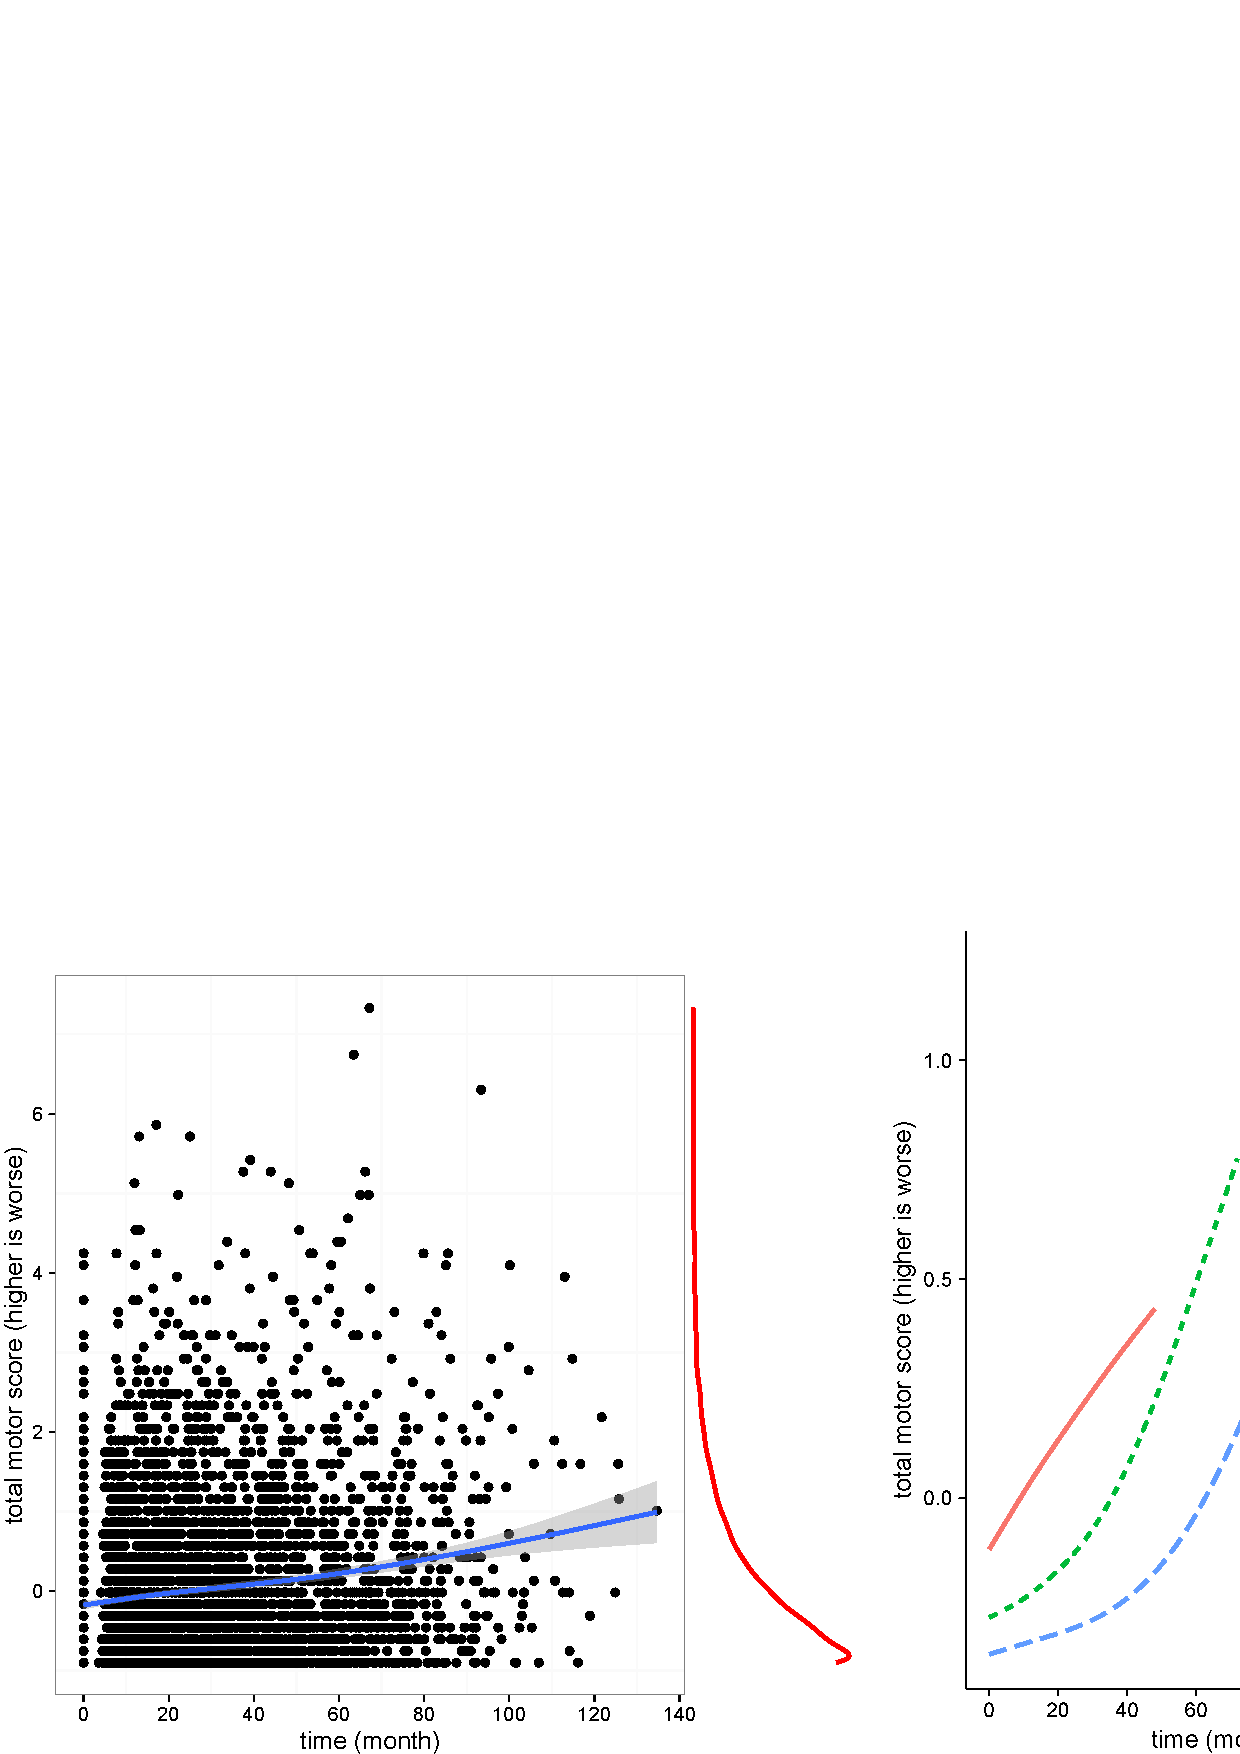
\includegraphics[width=\columnwidth]{TMS_scatter_loess_grp.pdf}
\caption{Left panel: Scatter plot (with loess curve) and kernel density plot (right side) for {total motor score} from the study population (time unit: month; lower total motor score is better); right panel: Mean total motor score values over time.}
\label{fig:data_neurotot}
\end{figure}

Moreover, we are specifically interested in estimating the risk of developing HD for those study participants who are still free of the disease. The JM framework offers a novel way of making such personalized dynamic predictions of future event-free probability \citep{rizopoulos2011dynamic,taylor2013real}. A key feature of these dynamic predictions frameworks is that the predictive measures can be dynamically updated as additional longitudinal measurements become available for the target subjects, providing instantaneous risk assessment. In order to make dynamic predictions in the LQMM-based JM framework, we develop a fully Bayesian algorithm for model estimation and dynamic predictions under the new quantile regression joint models (QRJM) framework. The algorithm consists of two parts. First, we build the QRJM framework consisting of an LQMM for the longitudinal process and a proportional hazard model (PHM) for the time to HD onset process and then draw Bayesian inference, based on a large study population. Second, we make predictions of future HD-free probability for a subject using his or her longitudinal biomarker trajectory information. To estimate the risk of a future event, we explore the posterior distribution of the fixed effects and the predictions of the subject-specific random effects from our QRJM. Moreover, we dynamically update the predictions as long as an individual is free of HD and new longitudinal measurements can be obtained. {Our work is different from \cite{farcomeni2015longitudinal} in the following: (1) we consider a fully Bayesian QRJM for statistical inference while \cite{farcomeni2015longitudinal} used a MCEM algorithm; (2) more importantly, by taking advantage of the posterior distributions of model parameters and subject-specif random effects, we develop a dynamic predictions procedure for future event-free probability under the proposed QRJM.}

The rest of this article proceeds as follows. In Section~\ref{sec:methods}, we give details of the QRJM and statistical methods used for inference and dynamic predictions. In Section~\ref{sec:simulation}, we present two simulation studies to validate the proposed methods. In Section~\ref{sec:data}, we apply the proposed methods to the motivating data set. We conclude the article with a discussion in Section~\ref{sec:discussion}.

% \bibliographystyle{plainnat}%%%%%%%%%%%%%%%%%%%%
% \addcontentsline{toc}{section}{References}
% \bibliography{QRJM}
% \end{document}




\subsection{Methods}\label{sec:methods}
\subsubsection{Bayesian Linear Quantile Mixed Model}\label{sec:BLQMM}%%%%%

Let $Y_{i}(t_{ij})$ be the longitudinal outcome for subject $i$ measured at time $t_{ij}$ where $i=1, \cdots, N\mbox{ and } j=1,\cdots, n_i$. Consider the linear mixed effects model:
\begin{equation}\label{eqn:lmm}
Y_{i}(t) ={\boldsymbol X}_{i}^{\top}(t) \boldsymbol{\beta}+ {\boldsymbol Z}_{i}^{\top}(t)\boldsymbol{u}_i + \varepsilon_{i}(t), \varepsilon_{i}(t)\sim N(0, \sigma^{2}),
\end{equation}
where $\boldsymbol{\beta}$ is a $p-$dimensional fixed effect vector,  ${\boldsymbol X}_{i}(t)$ contains the corresponding fixed covariates, $\boldsymbol{u}_i$ is a $k-$dimensional random effect vector for subject $i$, and ${\boldsymbol Z}_{i}(t)$ contains the corresponding random covariates.

A linear quantile mixed model (LQMM) assumes that the conditional quantile of the outcome is a linear function of the covariates,
\begin{equation}\label{eqn:lqmm}
Q_{Y_{i}(t)|{\boldsymbol X}_{i}(t),{\boldsymbol Z}_{i}(t)}(\tau)={\boldsymbol X}_{i}^{\top}(t) \boldsymbol{\beta}+ {\boldsymbol Z}_{i}^{\top}(t)\boldsymbol{u}_i,
\end{equation}
where the $\tau$th quantile of a random variable $Y$ is defined as $Q_{Y}(\tau)=F_{Y}^{-1}(\tau)=\inf\left\{ y:F_{Y}(y)\geq\tau\right\}$ for $\tau\in [0, 1]$. The quantile regression estimates can be obtained by minimizing the following loss function, $\hat{\boldsymbol{\beta}}_{\tau}=\underset{\boldsymbol{\beta}\in \mathbb{R}^{p}}{\mbox{arg min}}\sum_{i, t}\left[\rho_{\tau}\left(Y_{i}(t)-{\boldsymbol X}_{i}^{\top}(t)\boldsymbol{\beta} - {\boldsymbol Z}_{i}^{\top}(t)\boldsymbol{u}_i\right)\right]$, where $\rho_{\tau}(\cdot)$ is defined as $\rho_{\tau}(Y)=Y(\tau-{I}{(Y<0)})$. In quantile regression, parameter estimators are functions of the quantile. So parameter $\boldsymbol{\beta}_{\tau}$ is a function of quantile $\tau$, as denoted by the subscript.

As discussed in \citet{koenker1999goodness} and \citet{yu2001bayesian}, the above minimization problem can be rephrased as a maximum-likelihood problem by assuming that the random error $\varepsilon_{i}(t)$ in \eqref{eqn:lmm} follows the asymmetric Laplace distribution (ALD), denoted by $ALD(0, \sigma, \tau)$ with location parameter equals 0, scale parameter $\sigma>0$ and skewness parameter $\tau\in (0, 1)$. $ALD(0, \sigma, \tau)$ is skewed to left when $\tau>0.5$, and skewed to right when $\tau<0.5$. When $\tau=0.5$, ALD reduces to the symmetric Laplace distribution. To visualize this, Web Figure~1 displays the density functions of a standard normal distribution, a Laplace distribution, and two ALDs with $\tau=0.75$ and $\tau=0.25$, respectively. Adopting the ALD, the LQMM in \eqref{eqn:lqmm} becomes $Y_{i}(t) ={\boldsymbol X}_{i}^{\top}(t) \boldsymbol{\beta}_{\tau}+ {\boldsymbol Z}_{i}^{\top}(t)\boldsymbol{u}_i + \varepsilon_{i}(t), \varepsilon_{i}(t)\sim ALD(0, \sigma, \tau)$, where $i=1, \cdots, N$ and $t=1,\cdots, n_i$. The conditional likelihood function is $\ell(Y_{i}(t)|\boldsymbol{\beta}_{\tau},\boldsymbol{u}_i,\sigma)=\frac{\tau(1-\tau)}{\sigma}\exp\left[-\rho_{\tau}\left(\frac{Y_{i}(t)-{\boldsymbol X}_{i}^{\top}(t)\boldsymbol{\beta}_{\tau}-{\boldsymbol Z}_{i}^{\top}(t)\boldsymbol{u}_i}{\sigma}\right)\right]$.

Linear programming algorithms can be applied to obtain parameter estimates under the frequentist framework. However, to develop a Bayesian sampling algorithm for model inference, we utilize a location-scale mixture representation of the ALD (\citealp{kotz2001laplace}), which is a functional form with a mixture of common distributions. Under this parameterization, the random error is represented as $\varepsilon_{i}(t)=\kappa_1e_{i}(t)+\kappa_2\sqrt{\sigma e_{i}(t)}v_{i}(t)$ with $v_{i}(t)\sim \mathcal{N}(0,1), e_{i}(t)\sim\exp(1/\sigma)$, $\kappa_1=\frac{1-2\tau}{\tau(1-\tau)}$, and $\kappa_2^2=\frac{2}{\tau(1-\tau)}$.

This reparameterization leads to the following LQMM,
\begin{equation}\label{eqn:reformald2}
Y_{i}(t)={\boldsymbol X}_{i}^{\top}(t)\boldsymbol{\beta}_{\tau}+{\boldsymbol Z}_{i}^{\top}(t)\boldsymbol{u}_i+\kappa_1e_{i}(t)+\kappa_2\sqrt{\sigma e_{i}(t)}v_{i}(t),
\end{equation}
or equivalently, the conditional likelihood function is
%{\small
\begin{equation}\label{eqn:lo_sc_lh}
\ell(Y_{i}(t)|\boldsymbol{\beta}_{\tau},\boldsymbol{u}_i,e_{i}(t),\sigma)=\frac{1}{\sqrt{2\pi\kappa_2^2\sigma e_{i}(t)}}\exp\left[-\frac{(Y_{i}(t)-{\boldsymbol X}_{i}^{\top}(t)\boldsymbol{\beta}_{\tau}-{\boldsymbol Z}_{i}^{\top}(t)\boldsymbol{u}_i-\kappa_1e_{i}(t))^2}{2\kappa_2^2\sigma e_{i}(t)}\right].
\end{equation}
%}
As discussed in \cite{yu2001bayesian}, irrespective of the actual distribution of the data, Bayesian quantile regression using ALD distribution works quite well for different error distributions and the performance is quite robust and satisfactory.

\subsubsection{Joint Models Using Longitudinal Quantile Regression} %%%%%%%%%%%%%%%%%%%%%%%%%%%
We then extend the regular joint models (consisting of a linear mixed sub-model for the longitudinal process and a Cox proportional hazards model (PHM) submodel for the survival process, referred to as LMJM), by replacing the linear mixed sub-model with an LQMM as in \eqref{eqn:reformald2}. Let $T_i=min(T_i^*, C_i)$ be the observed event time for subject $i$, where $T_i^*$ is the true underlying event time and $C_i$ is the censoring time. Let $\Delta_i$ be the event indicator (1 if the event is observed, and 0 otherwise). Let $Y_{i}(t)$ be the continuous longitudinal outcome for subject $i$ measured at time $t$. Note that $Y_{i}(t)$ is only observed when $t\le T_i$, and the complete longitudinal measurements for subject $i$ can be written as $\mathcal{Y}_{i}(t)=\{Y_{i}(s): 0\le s\le t\}$. We denote the true underlying longitudinal measurement for subject $i$ at time $t$ with $m_{i}(t)$ and his/her complete history of true longitudinal process as $\mathcal{M}_{i}(t)=\{m_{i}(s): 0\le s \le t\}$. The proposed quantile regression joint models (QRJM) can be written as a set of two sub-models:
\begin{equation}\label{eqn:joint}
\left\{
\begin{array}{l}
Y_{i}(t) = m_{i}(t) + \varepsilon_{i}(t) = {\boldsymbol X}_{i}^{\top}(t)\boldsymbol{\beta}_{\tau} + {\boldsymbol Z}_{i}^{\top}(t){\boldsymbol u}_i + \varepsilon_{i}(t), \varepsilon_{i}(t)\sim ALD(0, \sigma, \tau)\\
h(T_i|\mathcal{M}_{i}(T_i), {\boldsymbol W}_i;  \boldsymbol{\gamma}_{\tau}, \alpha_{\tau}) = h_0(T_i)\exp({\boldsymbol W}_i^{\top}\boldsymbol{\gamma}_{\tau} + \alpha_{\tau}({\boldsymbol X}^{\top}_{i}(T_i)\boldsymbol{\beta}_{\tau} + {\boldsymbol Z}^{\top}_{i}(T_i){\boldsymbol u}_{i})),
\end{array}
\right.
\end{equation}
where the first sub-model is the LQMM introduced in Section \ref{sec:BLQMM}, in which $\boldsymbol{X}_{i}(t)$ are the fixed effect covariates and $\boldsymbol{Z}_{i}(t)$ are the covariates associated with $k-$dimensional multivariate normal random effects $\boldsymbol{u}_i$. The second sub-model takes the format of PHM where $h_0(\cdot)$ is the baseline hazard function and $\boldsymbol{W}_{i}$ are the $q-$dimensional fixed effect covariates only associated with event time (not the longitudinal outcome). These two sub-models are linked by incorporating $m_i(t)$ (the true underlying longitudinal measurement at time $t$) in the time-to-event process. The association parameter $\alpha_{\tau}$ quantifies the strength of association between $m_i(t)$ and the hazard for event at the same time point, e.g., positive $\alpha_{\tau}$ indicates that subjects with higher measurement tend to have an event earlier.

In the proposed QRJM \eqref{eqn:joint}, all parameters are functions of quantile $\tau$. Thus, by choosing different quantiles, one can conduct a comprehensive analysis of the relationship between the outcome and the covariates. Depending on the research aims, we can take different strategies to utilize the flexibility of the QRJM. For example, to conduct a study over the entire conditional distribution of the longitudinal outcome, we can just fit the QRJM through a set of selected quantiles, collect and compare the resulting parameter estimations. Less varying values in the parameter estimates indicates a relatively stable covariate effects on the outcomes, and vice versa. On the other hand, the interest may lie only in assessing the effect on some pre-specified quantiles (median, lower or higher quantile) of the longitudinal outcome and its association with the event process.

\subsubsection{The Survival Sub-model}\label{sec:surv_submodel}
For subject $i$, the likelihood function for survival data is:
\begin{eqnarray}\label{eqn:survival_like}
\ell(T_i, \Delta_i|\boldsymbol{{\boldsymbol u}_i}) =h(T_i|\mathcal{M}_{i}(T_i), \boldsymbol{W}_i)^{\Delta_i}S(T_i|\mathcal{M}_{i}(T_i), \boldsymbol{W}_i),
\end{eqnarray}
where $h(T_i|\mathcal{M}_{i}(T_i), \boldsymbol{W}_i)$ is given in \eqref{eqn:joint} and $S(\cdot)$ is the survival function,
\begin{equation*}
S(T_i|\mathcal{M}_{i}(T_i), \boldsymbol{W}_i)=\exp\left\{-\int_0^{T_i}h_0(s)\exp({\boldsymbol W_i}^{\top}\boldsymbol{\gamma}_{\tau} + \alpha({\boldsymbol X}_i^{\top}(s)\boldsymbol{\beta}_{\tau} + {\boldsymbol Z}_i^{\top}(s){\boldsymbol u}_{i}))ds\right\}.
\end{equation*}

For the baseline hazard $h_0(t)$, a parametric form such as exponential model can be used or it can be left unspecified. Specifically, we consider the piecewise-constant baseline hazard function, based on which a closed form survival function can be derived for each time interval. Further extension of the JM in the functional form of the two processes is also possible, as discussed in \citet{rizopoulos2014combining}. Although all parameters in the proposed QRJM are quantile dependent, for national ease and without ambiguity, we omit the subscript $\tau$ from all parameters in the following sections (e.g., $\boldsymbol{\theta}$ stands for $\boldsymbol{\theta}_{\tau}$ for all quantile-based parameters).

\subsubsection{Complete Likelihood Function and Bayesian Inference}\label{sec:estimation}
For subject $i$, the complete joint likelihood of the longitudinal and survival data can be written as
\begin{equation}\label{eqn:full_lik}
L_i(\boldsymbol{\theta};T_i, \Delta_i, \mathcal{Y}_{i}(T_i), \boldsymbol{u}_i) = \ell(\mathcal{Y}_{i}(T_i)|\boldsymbol{u}_i)\ell(T_i, \Delta_i|\boldsymbol{u}_i)f(\boldsymbol{u}_i|\boldsymbol{\Sigma}),
\end{equation}
where vector $\boldsymbol{\theta}$ represents all the parameters in \eqref{eqn:full_lik},  $\ell(\mathcal{Y}_{i}(T_i)|\boldsymbol{u}_i)=\prod_{0\le t\le T_i}\ell(Y_{i}(t)|\boldsymbol{u}_i)$, where $\ell(Y_{i}(t)|\boldsymbol{u}_i)$ is given in \eqref{eqn:lo_sc_lh}, and $\ell(T_i, \Delta_i|\boldsymbol{u}_i)$ is given in \eqref{eqn:survival_like}.

Parameter estimation can be made using Monte Carlo EM (MCEM) algorithm, in which random effects are treated as missing data (\citealp{farcomeni2015longitudinal}). In this article, however, we take advantage of the location-scale mixture representation of the ALD described in Section~\ref{sec:BLQMM} and propose a fully Bayesian inference approach for parameter estimation and personalized dynamic predictions. Given the complete likelihood in \eqref{eqn:full_lik} and by Bayes theorem, the posterior distributions of the model parameters are given by

\begin{equation}\label{eqn:posterior}
f(\boldsymbol{\theta}|\boldsymbol{T}, \boldsymbol{\Delta}, \boldsymbol{\mathcal{Y}}, \boldsymbol{u})\propto \prod_{i=1}^N L_i(T_i, \Delta_i, \mathcal{Y}_{i}(T_i), \boldsymbol{u}_i;\boldsymbol{\theta}) f(\boldsymbol{\theta}),
\end{equation}

\noindent where $\boldsymbol{T}=(T_1, T_2, \cdots, T_N)$, $\boldsymbol{\mathcal{Y}}=(\mathcal{Y}_{1}(T_1), \mathcal{Y}_{2}(T_2), \cdots, \mathcal{Y}_{N}(T_N))$, $\boldsymbol{\Delta} =(\Delta_1, \Delta_2, \cdots, \Delta_N)$, $\boldsymbol{u}=(\boldsymbol{u}_1, \boldsymbol{u}_2, \cdots, \boldsymbol{u}_N)$, and $f(\boldsymbol{\theta})=\pi(\boldsymbol{\beta})\pi(\boldsymbol{\gamma})\pi(\alpha)\pi(\sigma)\pi(\boldsymbol{\Sigma})$ is the product of the prior distributions,
where $\boldsymbol{\Sigma}$ is a $k\times k$ covariance matrix of the multivariate normal random effects distribution. We adopt the following prior distributions:
$\boldsymbol{\beta} \sim \mathcal{N}_p({\boldsymbol 0}, 10^3{\bf I}), \boldsymbol{\gamma} \sim \mathcal{N}_q({\boldsymbol 0}, 10^3{\bf I}), \alpha\sim \mathcal{N}(0, 10^3), \sigma\sim \mathcal{IG}(10^{-3}, 10^{-3}), \boldsymbol{\Sigma}^{-1}\sim Wishart({\bf I}, k+1).$ We also consider the Cholesky decomposition prior for $\boldsymbol{\Sigma}$ in our simulation studies and find similar results as Wishart prior gives (results not shown). We have investigated other selections of vague prior distributions with various hyper-parameters and obtained very similar results.

The advantages of using fully Bayesian approach include that the uncertainty of the parameter estimates is fully captured in the posterior distributions and no asymptotic theory is needed to derive the standard error. The fully Bayesian approach provides a straightforward framework to make subject-specific prediction of survival probability using the posterior samples of the parameters and of the posterior predictive distributions for the random effects. Moreover, the proposed QRJM can be readily implemented in \textsf{JAGS} software (version 4.0.0) (\citealp{plummer2003jags}) and the codes have been posted at the Web Supplement to facilitate easy reading and implementation of the proposed QRJM model.

\subsubsection{Predictions of Survival Probability}\label{sec:pred_survival}
Upon fitting the QRJM to a training dataset with $N$ subjects, we can make prediction of survival probability for a new subject based on a set of his or her historical longitudinal measurements (denoted by $\mathcal{Y}_{i}(t)$) as well as other covariates information. The conditional survival probability up to time $m = t+\Delta t$ ($\Delta t > 0$), given that the subject is event-free up to censoring time $t$, is denoted as $p_i(m|t) = Pr(T_i^*\ge m|T_i^*>t, \mathcal{Y}_{i}(t);\boldsymbol{\theta})$, which can be further elaborated as follows:
\begin{equation}\label{eqn:surv_prob_derv}
     \begin{aligned}
      & Pr(T_i^*\ge m|T_i^*>t, \mathcal{Y}_{i}(t);\boldsymbol{\theta})\\
      &=\int Pr(T_i^*\ge m|T_i^*>t, \mathcal{Y}_{i}(t), {\boldsymbol u}_i;\boldsymbol{\theta})
 {Pr({\boldsymbol u}_i|T_i^*>t, \mathcal{Y}_{i}(t);\boldsymbol{\theta})d{\boldsymbol u}_i}  \\
      &= {\int Pr(T_i^*\ge m|T_i^*>t, {\boldsymbol u}_i;\boldsymbol{\theta})Pr({\boldsymbol u}_i|T_i^*>t, \mathcal{Y}_{i}(t);\boldsymbol{\theta})d{\boldsymbol u}_i} \\
       &= {\int\frac{{S}_i[m|\mathcal{M}_{i}(m,{\boldsymbol u}_i, \boldsymbol{\theta});\boldsymbol{\theta}]}{{S}_i[t|\mathcal{M}_{i}(t,{\boldsymbol u}_i, \boldsymbol{\theta});\boldsymbol{\theta}]}Pr({\boldsymbol u}_i|T_i^*>t, \mathcal{Y}_{i}(t);\boldsymbol{\theta})d{\boldsymbol u}_i}, \\
     \end{aligned}
     \phantom{\hspace{0cm}}
\end{equation}
% }
where ${S}(\cdot)$ is the survival function conditional on the entire longitudinal history $\mathcal{M}_{i}(\cdot).$

To estimate \eqref{eqn:surv_prob_derv}, we can use the proposed Bayesian sampling algorithm in Section \ref{sec:estimation} to calculate the posterior mean of the prediction $E_{\boldsymbol{\theta}|\mathcal{D}_N}[p_i(m|t)]$ and
\begin{eqnarray}\label{eqn:expct_pred}
\nonumber E_{\boldsymbol{\theta}|\mathcal{D}_N}[p_i(m|t)]&=&Pr(T_i^*\ge m|T_i^*>t, \mathcal{Y}_{i}(t), \mathcal{D}_N)=\int Pr(T_i^*\ge m|T_i^*>t, \mathcal{Y}_{i}(t);\boldsymbol{\theta})p(\boldsymbol{\theta}|\mathcal{D}_N)d\boldsymbol{\theta},
\end{eqnarray}
where $\mathcal{D}_N=\{T_i, \Delta_i, \boldsymbol{Y}_i, i=1, \cdots, N\}$ denotes the training data of size $N$ and the first part of the equation is given in \eqref{eqn:surv_prob_derv}.

A Monte Carlo (MC) estimate of $p_i(m|t)$ can be obtained using the following procedure:
\begin{enumerate}
\item Draw $\boldsymbol{\theta}^{(p)} \sim Pr(\boldsymbol{\theta}|\mathcal{D}_N)$ for $p=1, \cdots, P$;
\item For each $\boldsymbol{\theta}^{(p)}$, draw ${\boldsymbol u}^{(q)}_i\sim f({\boldsymbol u}_i|T_i^*>t, \mathcal{Y}_{i}(t), \boldsymbol{\theta}^{(p)})$ for $q=1, \cdots, Q$ and compute $$p_i^{(p)}(m|t)=\frac{1}{Q}\sum_{q=1}^QS_i[m|\mathcal{M}_{i}(m, \boldsymbol{u}^{(q)}_i, \boldsymbol{\theta}^{(p)});\boldsymbol{\theta}^{(p)}]S_i[t|\mathcal{M}_{i}(t, \boldsymbol{u}^{(q)}_i, \boldsymbol{\theta}^{(p)});\boldsymbol{\theta}^{(p)}]^{-1};$$
\item Approximate $p_i(m|t)$ by $\hat{p}_i(m|t)=\frac{1}{P}\sum_{p=1}^P p^{(p)}_i(m|t)$ after collecting all $P$ samples of $p_i(m|t)^{(p)}$.
\end{enumerate}

In above algorithm, $P$ is the total number of MC iterations, $f(\boldsymbol{\theta}|\mathcal{D}_N)$ is the posterior distributions of $\boldsymbol{\theta}$ given in \eqref{eqn:posterior}, and $f({\boldsymbol u}_i|T_i^*, \mathcal{Y}_{i}(t), \boldsymbol{\theta}^{(k)})$ is the posterior distribution of the random effects for subject $i$. And the uncertainty of the predictions is captured in the sample variance.

The posterior predictive values of the random effects ${\boldsymbol u}_i$ are direct results from the MCMC iterations if the subject is from the training dataset. For a new subject who is not in the training dataset, we can use the inference results to run additional MCMC iterations to obtain samples for the new subject's random effects ${\boldsymbol u}_i$ and the rest of the algorithm follows. Because each individual only has a few random effects (two in our current model) to estimate, a short MCMC with 200 iterations should be sufficient for convergence (\citealp{taylor2013real}).

\subsubsection{Predictive Accuracy} \label{sec:pred_accuracy}
Predictive accuracy of a model can be evaluated from different perspectives, such as discrimination (how well the models discriminate between subjects who had the event from those who did not), validation (how well the models predict the observed data), and reclassification (how well the model prediction improves by adding new predictors). Here we mainly focus on the discriminative ability of our model. Area under the receiver operating characteristic curve (AUC) is a commonly used statistics to evaluate the discriminative ability in prediction, while above average risk difference (AARD) measures the difference in the risk rates comparing events versus non-events at the level of population average risk, and mean risk difference (MRD) is the average difference between true positive rate (TPR) and false positive rate (FPR) across the risk scale (\citealp{pepe2008comments}). Higher values in AUC, AARC, and MRD indicate better discriminative ability. We use all three measurements as summary statistics to evaluate the discriminative performance of our model.

Following \citet{zheng2013adopting} and \citet{yang2015prediction}, at a given time $t$, a future time $ m = t+\Delta t$, and a threshold $c$, the TPR and FPR of the predictive results can be defined as $\mbox{TPR}_t(c)=Pr({\bf 1}-\boldsymbol{p}(m|t)\ge c | \boldsymbol{T}\le m)$ and $\mbox{FPR}_t(c)=Pr({\bf 1}-\boldsymbol{p}(m|t)\ge c | \boldsymbol{T} > m)$, where $\boldsymbol{p}(m|t)=\{p_i(m|t), i=1, \ldots, N\}$ and $p_i(m|t)$ is illustrated in Section~\ref{sec:pred_survival}. The estimate of $\boldsymbol{p}(m | t)$ is denoted by $\hat{\boldsymbol{p}}(m | t)$, and the estimators of TPR and FPR are: $\widehat{TPR}_{t}(c) = \frac{\sum_{i=1}^{N}(1-\hat{p}_i(m|t))I(1-\hat{p}_i(m|t)\ge c)}{\sum_{i=1}^{N}(1-\hat{p}_i(m|t))}$ and $\widehat{FPR}_{t}(c) = \frac{\sum_{i=1}^{N}\hat{p}_i(m|t)I(1-\hat{p}_i(m|t)\ge c)}{\sum_{i=1}^{N}\hat{p}_i(m|t)}$. By definition, we have $\widehat{AUC}_t = \int \widehat{TPR}_t\left\{ (\widehat{FPR}_t)^{-1}(u)\right\}du$, $\widehat{AARD}_t = \widehat{TPR}_t(\hat{\rho}) - \widehat{FPR}_t(\hat{\rho})$, and $\widehat{MRD}_t = \int_c \widehat{TPR}_t(c)dc - \int_c \widehat{FPR}_t(c)dc$, where $\hat{\rho} = \frac{\sum_{i=1}^N (1-\hat{p}_i(m| t))}{N}$ is the average risk in the study population at time $m$.





%All is done in \LaTeX \cite{knuth1986texbook}.
%
%
% \bibliographystyle{plainnat}%%%%%%%%%%%%%%%%%%%%
% \addcontentsline{toc}{section}{References}
% \bibliography{QRJM}


% \end{document}
% \documentclass{article}
% \usepackage[utf8]{inputenc}
% \usepackage{fullpage}
% \usepackage{setspace}
% \usepackage[hang,flushmargin]{footmisc} %control footnote indent
% \usepackage{url} % for Appendicessite links
% \usepackage{amssymb,amsmath}%for matrix
% \usepackage{graphicx}%for figure
% \usepackage{appendix}%for appendix
% \usepackage{float}
% \floatstyle{plaintop}
% \restylefloat{table}
% \usepackage{multirow}
% \usepackage{longtable}
% \usepackage{morefloats}%in case there are too many float tables and figures
% \usepackage{caption}
% \usepackage{subcaption}
% \usepackage{listings}
% \captionsetup[subtable]{font=normal}
% \usepackage{color}
% \usepackage{hyperref}
% \usepackage[round]{natbib}
% \usepackage{rotating} % rotate table by some degree
% \usepackage{rotfloat}



% %\usepackage{Sweave}
% \setlength{\parindent}{0em}
% \setlength{\parskip}{0.5em}


% \graphicspath{{0.plots/}}



% \begin{document}

%%%%%%%%%%%%%%%%%%%%%%%%%%%%%%%%%%%%
\subsection{Simulation Studies} \label{sec:simulation}
%%%%%%%%%%%%%%%%%%%%%%%%%%%%%%%%%%%%
We conduct two simulation studies to validate the proposed QRJM. In the first simulation study, we assess the performance of the proposed Bayesian method in terms of bias and precision of the parameter estimates. In the second simulation study, we assess the predicted survival probability by comparing with the ``gold standard'' calculated based on the true (simulated) values of random effects and parameters.

%%%%%%%%%%%%%%%%%%%%%%%%%%%%%%%%%%%%
\subsubsection{Simulation Study I: Inferential Performance }\label{sec:sim1}
%%%%%%%%%%%%%%%%%%%%%%%%%%%%%%%%%%%%
In this simulation study, we consider different simulation scenarios where the random errors are generated from either a standard normal distribution or ALD distributions at different quantile $\tau$. The simulated data are then fitted using our proposed QRJM (assuming ALD for the random errors) as well as the LMJM (assuming normality for the random errors).


We let the covariate vectors in Model \eqref{eqn:joint} be ${\boldsymbol Z}_i(t)=(1, t)^{\top}, {\boldsymbol X}_i(t)=(1, x_{i1}, x_{i2}\cdot t)^{\top}, \mbox{ and } {\boldsymbol W}_{i}=(w_{i1}, w_{i2})^{\top}$ with covariates $x_{i1}, x_{i2}, w_{i1}$ and $w_{i2}$ being generated from independent standard normal distributions. We simulate the random effects, $\boldsymbol{u}_i$, from a bivariate normal distribution with mean vector {\bf 0}, and standard deviations both equal to 0.3 and correlation coefficient equals to 0.16.

To simulate the survival time, we choose constant baseline hazard. We obtain event time $T_i$ by inverting the survival function after generating $n$ random values from the standard uniform distribution. We generate the censoring time $C_i$ from $\textnormal{Beta}(4,1)$ to obtain a censoring proportion around 25\%. The longitudinal data are simulated from either a standard normal distribution or a ALD with the location parameter being $\boldsymbol{\beta}^{\top}{\boldsymbol X}_i(t) + {\boldsymbol u}_i^{\top}{\boldsymbol Z}_i(t)$ and dispersion parameter being $\sigma=1$. We keep a maximum of 6 observations for each subject, at follow-up time $t=(0, 0.25, 0.5, 0.75, 1, 3)$ respectively, after incorporating the time-to-event information.

We consider the following three scenarios in simulation study I:
\begin{enumerate}
\item Scenario 1: random errors follow the ALD with $\tau=0.25$ (right-skewed);
\item Scenario 2: random errors follow the ALD with $\tau=0.5$ (symmetric about 0 with heavy tails);
\item Scenario 3: random errors follow a standard normal distribution (symmetric about 0).
\end{enumerate}

In each scenario, we simulate 200 datasets with $N=600$ in each. Among the 600 subjects, we randomly select 500 subjects as the training dataset to build the model, and use the remaining 100 subjects as the validation dataset to make out-of-sample predictions.

We report bias, standard error (SE), mean squared error (MSE), and coverage probability (CP) for the QRJM and LMJM. Table~\ref{tab:sim1tab1} suggests that in Scenario 1, the true model (QRJM with $\tau=0.25$) provides parameter estimates with very small biases and CP being close to the nominal level. In comparison, the QRJM with $\tau=0.5$ provides reasonable estimates for most parameters, except the intercept $\beta_0$. The poor estimate of $\beta_0$ (large bias and CP far from 0.95) should not be surprising because of the incorrect specification of quantile $\tau$. The LMJM results in very biased estimates and the CP being away from the nominal value 0.95 (especially in regression parameters $\boldsymbol{\beta}$ in the longitudinal model). In Scenario 2 (see Appendices Table~\ref{tab:sim1tab2}) when data are symmetrical about 0 with heavier tails than the normal distribution, the LMJM still produces notably larger bias and lower CP as compared to the true model QRJM with $\tau=0.5$. In Scenario 3 (see Appendices Table~\ref{tab:sim1tab3}), median regression (the QRJM with $\tau=0.5$) performs comparably to the true model LMJM, suggesting that the QRJM can provide reasonable estimates when normality assumption holds. For completion, we also consider a scenario where the random errors are simulated from ALD with $\tau=0.75$ (left-skewed). The results (not presented) are very similar to Scenario 1, i.e., the true model QRJM with $\tau=0.75$ provides reasonable estimates while LMJM gives biased estimates and CP being far away from 0.95.
% latex table generated in R 3.2.2 by xtable 1.7-4 package
% Tue Oct 27 23:05:22 2015
\begin{table}[H]
% \begin{center}
\caption{Simulation results in Simulation study I Scenario 1 in which random errors are generated from ALD with $\tau=0.25$.}
\adjustbox{max width=\textwidth}{
\label{tab:sim1tab1}
\begin{tabular}{lrcccccccccccccc}
\hline
& \multicolumn{4}{c}{QRJM ($\tau=0.25$)} & & \multicolumn{4}{c}{QRJM ($\tau=0.5$)} & & \multicolumn{4}{c}{LMJM}\\
\hline
 & Bias & SE & MSE & CP && Bias & SE & MSE & CP && Bias & SE & MSE & CP \\
  \hline
  \multicolumn{10}{l}{Coefficients for longitudinal process} \\
  $\beta_0$ & $-$0.003 & 0.080 & 0.014 & 0.930 && 1.659 & 0.129 & 2.807 & 0.020 && 2.702 & 0.146 & 7.350 & 0.000 \\
  $\beta_1$ & 0.015 & 0.068 & 0.010 & 0.950 && 0.024 & 0.105 & 0.043 & 0.890 && 0.080 & 0.116 & 0.052 & 0.860  \\
  $\beta_2$ & 0.016 & 0.083 & 0.013 & 0.950 && 0.014 & 0.112 & 0.042 & 0.970 && 0.078 & 0.128 & 0.052 & 0.920  \\
  \multicolumn{10}{l}{Coefficients for survival process} \\
  $\gamma_1$ & 0.005 & 0.055 & 0.006 & 0.940 && 0.008 & 0.057 & 0.006 & 0.960 && 0.009 & 0.058 & 0.007 & 0.960  \\
  $\gamma_2$ & 0.006 & 0.055 & 0.006 & 0.930 && 0.010 & 0.056 & 0.007 & 0.910 && 0.010 & 0.058 & 0.007 & 0.940  \\
  $\alpha$ & $-$0.004 & 0.078 & 0.010 & 0.970 && $-$0.051 & 0.119 & 0.070 & 0.930 && $-$0.087 & 0.103 & 0.040 & 0.800  \\
   \hline
\end{tabular}
}
% \end{center}
\end{table}


%%%%%%%%%%%%%%%%%%%%%%%%%%%%%%%%%%%%
\subsubsection{Simulation Study II: Predictive Performance}\label{sec:sim2}
%%%%%%%%%%%%%%%%%%%%%%%%%%%%%%%%%%%%
In this simulation study, we make predictions for 100 subjects in the validation dataset (out-of-sample predictions) in the three scenarios in Section\ref{sec:sim1}. For each subject, we use the simulated data, random effects and the true parameter values to calculate the true survival probability given by $\frac{S_i[m|\mathcal{M}_{i}(m, {\boldsymbol u_i}, \boldsymbol{\theta});\boldsymbol{\theta}]}{S_i[t|\mathcal{M}_{i}(t, {\boldsymbol u_i}, \boldsymbol{\theta});\boldsymbol{\theta}]}$ and we use it as the ``gold standard''.

To assess the prediction validation (how well the models predict the survival probability), we use a Bland-Altman plot, a commonly used method to assess the agreement of the results from two measurement methods \citep{bland1986statistical}. To make the predictions ``dynamic'', we choose different combinations of censoring time (i.e., $t$) and the prediction time interval (i.e., $\Delta t$) to mimic expected real-world time points based on our HD data set. Appendices Figure~\ref{plot:sim2fig2} gives an intuitive comparison of the predicted results with the ``gold standard'' among different models. Plots from the true model (Appendices Figure~\ref{plot:sim2fig11}) are horizontally spindle-shaped, suggesting that it is easier to predict a probability near 0 or 1 than the middle probability area near 0.5. Further, with an increase in $\Delta t$, there is more variation in the middle probability area, indicating that survival probability predictions for time points further into the future are less accurate than predictions for closer time points, as expected. Bland-Altman plots from the other models (QRJM with $\tau=0.5$, Appendices Figure~\ref{plot:sim2fig12} and LMJM, Appendices Figure~\ref{plot:sim2fig13}) display systematically biased patterns in predictions.

Table~\ref{tab:sim2tab1} summarizes the comparison from the Bland-Altman plots for three chosen censoring time points ($t=0.25, 0.5, 0.75$). With longer follow-up time, we tend to have more longitudinal measurements per subject and tend to have more precise predictions.On the other hand, longer follow-up time leads to fewer subjects left in the study due to event occurrence and censoring (presented as a percentage in the first column of Table~\ref{tab:sim2tab1}), which results in higher variability in predictions. For example, in Table~\ref{tab:sim2tab1}, at $t=0.25$, there are 48.1\% subjects remain and at $t=0.5$ and 0.75, only 34.6\% and 22.8\%, respectively, of the subjects remain. As a result, we see comparable prediction results at $t=0.25$ and 0.5 but worse predictive performance when $t$ increases to 0.75. This is because the effect of additional longitudinal observations is ``canceled out'' by the variability from fewer subjects. Similarly, from the Bland-Altman plots, under the true model at the same censoring time $t$, an increase in $\Delta t$ leads to larger bias and MSE (Appendices Figure~\ref{plot:sim2fig11}). Because Table~\ref{tab:sim1tab1} suggests that the predictions from other models (QRJM with $\tau=0.5$ and LMJM) are systematically biased, their MSE and bias in Table~\ref{tab:sim2tab1} are much larger than the true model QRJM with $\tau=0.25$. Prediction results for Scenario 3 can be found in Appendices Table~\ref{tab:sim2tab2} and Appendices Figure~\ref{plot:sim2fig2}, in which QRJM with $\tau = 0.5$ performs comparably well as the true model when random errors are generated from standard normal distribution.

In summary, when data are simulated from ALD with specific skewness $\tau$, the best predictions of survival probability are obtained using the QRJM model with the exact quantile that generated the outcome data. Instead, LMJM results in systematically biased predictions when data are skewed. When random errors are standard normally distributed, predictions from QRJM with $\tau=0.5$ are comparable with those from the true model.

\begin{table}[H]
\centering
\caption{Simulation study: MSE and bias of the difference between predicted survival probability and the gold standard (Scenario 1).}
\adjustbox{max width=\textwidth}{
\label{tab:sim2tab1}
\begin{tabular}{clcccccccc}
\hline
 & & \multicolumn{2}{c}{QRJM ($\tau=0.25$)} & &\multicolumn{2}{c}{QRJM ($\tau=0.5$)} & &\multicolumn{2}{c}{LMJM} \\
\cline{3-4}\cline{6-7}\cline{9-10}
$t$ & $\Delta t$ & MSE & Bias & & MSE & Bias & & MSE & Bias \\
\hline
\multirow{2}{*}{{\bf 0.25}} & 0.25 & 0.006 & 0.009 && 0.137 & $-$0.330 & & 0.244 & $-$0.462 \\
&  1 & 0.010 & 0.007 && 0.111 & $-$0.267 & & 0.177 & $-$0.343 \\
\multirow{2}{*}{(subjects left: 48.1\%)} &  2 & 0.012 & 0.003 && 0.083 & $-$0.197 & & 0.126 &$-$0.249 \\
&  3 & 0.013 & 0.000 && 0.072 & $-$0.168 & & 0.107 & $-$0.210 \\
\hline
\multirow{2}{*}{{\bf 0.5}} & 0.25 & 0.007 & 0.009 && 0.130 & $-$0.317 & & 0.219 & $-$0.439 \\
&   1 & 0.015 & 0.000 && 0.144 & $-$0.321 & & 0.221 & $-$0.408 \\
\multirow{2}{*}{(subjects left: 34.6\%)}&   2 & 0.017 & $-$0.015 && 0.121 & $-$0.259 & & 0.174 & $-$0.319 \\
&   3 & 0.018 & $-$0.023 && 0.109 & $-$0.228 & & 0.153 & $-$0.278\\
\hline
\multirow{2}{*}{{\bf 0.75}} & 0.25 & 0.009 & 0.005 && 0.125 & $-$0.301 & & 0.189 & $-$0.401 \\
& 1 & 0.023 & $-$0.007 && 0.174 & $-$0.356 & & 0.253 & $-$0.447 \\
\multirow{2}{*}{(subjects left: 22.8\%)} & 2 & 0.025 & $-$0.033 && 0.159 & $-$0.310 & & 0.218 & $-$0.375 \\
&  3 & 0.027 & $-$0.046 && 0.148 & $-$0.282 & & 0.197 & $-$0.336\\
\hline
\end{tabular}
}
\end{table}






% \begin{figure}[H]
% \centering
% \includegraphics[width=0.45\textwidth]{baplot_qt25data_qt25fit_jags_t1.pdf}
% \includegraphics[width=0.45\textwidth]{baplot_qt25data_qt50fit_jags_t1.pdf}
% \hline
% \includegraphics[width=0.45\textwidth]{baplot_qt25data_LMJMfit_arms_t1.pdf}
% \includegraphics[width=0.45\textwidth]{baplot_qt25data_JMbayesfit_t1.pdf}
% \label{plot:sim2fig1}
% \caption{BA plot of predictions with first two longitudinal observations ($t$=0.25) from true model (top left), QRJM with $\tau=0.5$(top right), LMJM (bottom left) and \LMJM(bottom right), Scenario One}
% \end{figure}










%
%
%All is done in \LaTeX \cite{knuth1986texbook}.
%
%
% \bibliographystyle{plainnat}%%%%%%%%%%%%%%%%%%%%
% \addcontentsline{toc}{section}{References}
% \bibliography{QRJM}

% \end{document}
% \documentclass{article}
% % \usepackage[utf8]{inputenc}
% \usepackage{fullpage}
% \usepackage {setspace}
% \usepackage[hang,flushmargin]{footmisc} %control footnote indent
% \usepackage{url} % for Appendicessite links
% \usepackage{amssymb,amsmath}%for matrix
% \usepackage{graphicx}%for figure
% \usepackage{appendix}%for appendix
% \usepackage{float}
% \usepackage{multirow}
% \usepackage{longtable}
% \usepackage{morefloats}%in case there are too many float tables and figures
% \usepackage{caption}
% \usepackage{subcaption}
% \usepackage{listings}
% \captionsetup[subtable]{font=normal}
% \usepackage{color}
% \usepackage{hyperref}
% \usepackage[round]{natbib}
% \usepackage[export]{adjustbox}
% %\usepackage{Sweave}
% \setlength{\parindent}{0em}
% \setlength{\parskip}{0.5em}


% \graphicspath{{0.plots/}}


% \begin{document}
\subsection{Application}\label{sec:data}

%%%% briefly talk about which data will be used then talk about clinical background of HD
\subsubsection{The Predictors of Huntington's Disease (PREDICT-HD) Study}\label{sec:data_analysis}
The motivating PREDICT-HD study is an observational study that aims to identify the earliest signs of HD onset so that future HD drug trials can be targeted toward treatment that may slow the progression of the disease, or prevent it altogether \citep{paulsen2008detection}. Briefly, HD is known to be caused by the mutation of the first exon of the Huntington (HTT) gene, where expansion of the cytosine-adenine-guanine (CAG) is observed for HD patients.\par

%%%% More details on the PREDICT-HD study and the data set: longitudinal part and time-to-event part
The study recruited participants from 33 medical centers in six countries (i.e., USA, Canada, Germany, Australia, Spain, and UK) starting from August, 2002. Qualified participants were healthy pre-HD people without any symptoms of HD; i.e., who have not had a motor diagnosis of HD based on the Unified Huntington Disease Rating Scale (UHDRS) and had more than 35 HTT CAG repeats. Detailed inclusion and exclusion criteria can be found in \cite{paulsen2006preparing}. Baseline demographic information such as age, gender, education years, as well as clinical variables such as CAG repeat length and Beck Depression Inventory were recorded at enrollment. A total of 40 longitudinal biomarkers from five domains (i.e., motor, cognitive, psychiatric, functional, and imaging) were recorded. The data used in the current study contains 1078 individuals enrolled until July, 2014. Among those 1078 participants, 64\% are female and the mean age at baseline is 39.8 years (SD=10.39, range 18.1-83.7), education is 14.5 years (SD=2.60, range 8.0-20.0), and number of CAG repeats is 42.5 (SD=2.69, range 12-62). In this study, the time variable is defined as months since enrollment. The average follow-up time is 61.2 months (SD=39.6; range 0.12-144.0) and 959 (89\%) participants have data for at least two years. The survival event of interest is motor diagnosis of HD since enrollment, which is defined as having a diagnostic confidence level (DCL) score of 4 (the highest score)\citep{paulsen2014prediction}. During the study follow-up, 225 (21\%) events (HD onsets) were observed.



%%%% put demographic table here
% Table~\ref{tab:data} summaries the baseline demographics of the study cohort.

% \begin{table}[H]
% \centering
% \caption{Baseline demographics of the study cohort \citep{paulsen2014prediction}}
% \label{tab:data}
% \begin{adjustbox}{width=\textwidth,totalheight=\textheight,keepaspectratio}
% \begin{tabular}{llp{5cm}p{5cm}}
% \hline
%  Variable & Study cohort & Participants not diagnosed with HD during the study (n=835) & Participants diagnosed with HD during the study (n=225)\\
%  \hline
%  Women & 687(64\%) & 540(63\%) & 147(65\%)\\
%  Age (years) & 39.78(10.39) & 38.92(10.24)  & 43.03(10.31) \\
%  CAG repeat length & 42.49 (2.69)& 42.21(2.58)& 43.57(2.85)\\
%  CAP & 356.12(92.30) & 334.89(82.74)& 436.59(81.82)\\
%  Education (years) & 14.46(2.60)& 14.56(2.62) & 14.08(2.50)\\
%  Time in study (years) & 4.78(3.30)&  4.28(3.31) & 6.66(2.48)\\
%  \hline
% \end{tabular}
% \end{adjustbox}
% \end{table}

We select five longitudinal biomarkers, one from each domain, that are known to be strongly predictive of HD onset \citep{paulsen2014prediction} (see Appendices Section~3 for variable definitions). In the exploratory data analysis, we plot the scatter plots (with loess curves) and the kernel density plots of those selected variables (see Figure~\ref{fig:data_neurotot} and Appendices Figure~4). The distributions of TMS, {FrBe Executive Subscale} (FES), and {Total Functional Capacity} (TFC) all clearly deviate from normality, indicating a strong indication that the LMM may not be appropriate for these outcomes. From the loess curves, we observe the general direction of association between each longitudinal biomarker and the risk of HD onset. For example, {putamen} volume (intracranial-corrected) decreases over time and the brain atrophy from decreased putamen volume is associated with increased hazard of HD onset \cite{paulsen2014prediction}. To compare the longitudinal results on the same scale, we have standardized all longitudinal biomarkers.



We consider the following joint model for our data analysis:
\begin{equation*}\label{eqn:data_joint}
\left\{
\begin{array}{l}
y_{i}(t) = m_{it} + \varepsilon_{it} = \beta_0 + \beta_1 t+ \beta_2 age_{0i} + {u}_{i1} + u_{i2} t + \varepsilon_{i}(t),  \varepsilon_{i}(t)\sim ALD(0, \sigma, \tau)\\
h(T_i|\mathcal{M}_{iT_i};  \boldsymbol{\gamma}, \alpha) = \sum_{k=1}^3\lambda_kI_k(T_i)\exp(\gamma_1 education_i + \gamma_2 I_{male_i} + \alpha m_i(T_i))
\end{array}
\right.
\end{equation*}
where $y_{i}(t)$ represents one of the five selected longitudinal biomarkers and $age_i$ is the baseline age of subject $i$. In the survival sub-model, we specify a piecewise constant baseline hazard function with three time intervals, where $\lambda_k$ is the hazard rate for time interval $[t_k, t_{k+1})$ and $I_k(t)=1$ if $t\in[t_k, t_{k+1})$ and 0 otherwise.We have explored different numbers of time intervals and pieces and have obtained very similar results.

We randomly split the 1078 study participants into two datasets: a training dataset of 800 participants to draw statistical inference for the unknown parameters and a validation dataset of 278 participants for predictions of HD-free probability. In the model fitting step, two chains are initiated with diverse initial values and the chains are considered to converge if the potential scale reduction factors (PSRF) \citep{brooks1998general} for all parameters are below 1.1. In the prediction step we choose different censoring time ($t$) and prediction time window ($\Delta t$) combinations (similar to those chosen in the simulation study). Predictive accuracy for the test cohort is summarized using AUC, AARD ,and MRD defined in Section~\ref{sec:pred_accuracy} for each ($t, \Delta t$) combination as well as for each quantile in the QRJM. We also calculate the AUCs from the LMJM and compare them with those from our QRJM model.



\subsubsection{Inference Results for PREDICT-HD data}\label{sec:data_results}
Table~\ref{p1realdata_inference} (for the outcome TMS) and Appendices Table 4 (for the outcomes putamen, stroop word, FES, and TFC) present the inference results from the QRJMs at $\tau=$ 0.25, 0.50, and 0.75. In the longitudinal process, the coefficient for time quantifies the change rate of a specific longitudinal biomarker at a fixed quantile. For example, Table~\ref{p1realdata_inference} suggests that the time effect is 0.019 (95\% CI: 0.015, 0.023) for TMS at $\tau=0.25$, indicating one month increase in time is associated with 0.019 unit increase of TMS (when $\tau=0.25$). The positive time coefficients for TMS at all quantiles indicate that TMS increases (deteriorates) over time, which is consistent with the loess curves in Figure~\ref{fig:data_neurotot}. The magnitude of the time coefficient is similar at different quantiles for TMS, putamen, stroop word, and FES, indicating comparable progression in each of these outcomes at those quantiles. However, some variability is observed in TFC, where the time effect is highest at lower quantiles of TFC and becomes smaller at higher quantiles. Because lower TFC is associated with higher risk of HD onset, and these data indicate that the health of those with lower TFC deteriorates faster, special targeted care may be needed for those individuals in the lower quantile of TFC, in order to reduce their risk of HD onset.

Table~\ref{p1realdata_inference} also suggests that higher baseline age is associated with higher (worse) TMS and one year increase in baseline age is associated with 0.005 (95\% CI: 0.001, 0.010) units increase in TMS (when $\tau=0.5$). In the time-to-event process, across all three quantiles, education has protective effect on HD onset, i.e., those with more education years tend to have a lower risk of HD onset. Outcome TMS is strongly predictive of HD onset at all quantiles. Specifically, an unit increase in TMS increases the risk of HD onset by 4.600 ($\exp(1.526)$, 95\% CI 3.747-5.726) times at $\tau=0.25$, by 3.669 (95\% CI 3.152-4.302) times at $\tau=0.5$, and by 2.945 (95\% CI 2.633-2.294) times at $\tau=0.75$, respectively. Similarly, worse outcomes in putamen, stroop word task, FES, and TFC are also strongly associated with higher risk of HD onset across all quantiles.


% latex table generated in R 3.2.0 by xtable 1.8-0 package
% Mon Jan 11 22:29:09 2016
% \begin{table}[H]
% \centering
% \caption{Model estimations from QRJM with different quantiles of {Total motor score} in the longitudinal process.}
% \label{realdata_neurotot}
% \begin{tabular}{rrrrrr}
%   \hline
%  & Lower95 & Median & Upper95 & Mean & SD \\
%   \hline
%   \multicolumn{6}{c}{$\tau=0.25$}\\
%   \hline
%   \multicolumn{2}{l}{\textit{longitudinal process}} & & & &\\
%   int. & -0.652 & -0.614 & -0.574 & -0.614 & 0.020\\
%   time & 0.014 & 0.019 & 0.023 & 0.019 & 0.003\\
%   \multicolumn{2}{l}{\textit{time-to-event process}} & & & &\\
%   assoct. & 1.137 & 1.295 & 1.465 & 1.298 & 0.083 \\
%   eduyr & -0.124 & -0.093 & -0.068 & -0.095 & 0.015\\
%   % gamma2[1] & 0.000 & 0.000 & 0.000 & 0.000 & 0.000 &  \\
%   male & -0.040 & 0.335 & 0.715 & 0.333 & 0.193\\
%    \hline
%      \multicolumn{6}{c}{$\tau=0.50$}\\
%   \hline
%   \multicolumn{2}{l}{\textit{longitudinal process}} & & & &\\
%   int. & -0.364 & -0.317 & -0.270 & -0.317 & 0.024 \\
%   time & 0.015 & 0.020 & 0.024 & 0.020 & 0.002 \\
%   \multicolumn{2}{l}{\textit{time-to-event process}} & & & &\\
%   assoct. & 1.027 & 1.164 & 1.306 & 1.167 & 0.071 \\
%   eduyr & -0.154 & -0.124 & -0.099 & -0.125 & 0.014 \\
%   % gamma2[1] & 0.000 & 0.000 & 0.000 & 0.000 & 0.000 &  \\
%   male & -0.079 & 0.300 & 0.671 & 0.300 & 0.193 \\
%    \hline
%         \multicolumn{6}{c}{$\tau=0.75$}\\
%   \hline
%   \multicolumn{2}{l}{\textit{longitudinal process}} & & & &\\
%   int. & -0.050 & 0.007 & 0.062 & 0.007 & 0.028 \\
%   time & 0.016 & 0.021 & 0.025 & 0.021 & 0.002 \\
%   \multicolumn{2}{l}{\textit{time-to-event process}} & & & &\\
%   assoct. & 0.901 & 1.009 & 1.115 & 1.009 & 0.055 \\
%   eduyr & -0.174 & -0.145 & -0.119 & -0.146 & 0.014 \\
%   % gamma2[1] & 0.000 & 0.000 & 0.000 & 0.000 & 0.000 &  \\
%   male & -0.169 & 0.200 & 0.560 & 0.199 & 0.188\\
%    \hline
% \end{tabular}
% \end{table}


% \begin{sidewaystable}
\begin{table}[H]
\centering
\caption{PREDICT-HD data analysis: Parameter estimation and 95\% credible interval (in parenthesis) from QRJM at three different quantiles with TMS being the longitudinal biomarker.}
\label{p1realdata_inference}
\resizebox{\linewidth}{!}{
\begin{tabular}{lccc}
  \hline
  % & \multicolumn{3}{c}{{total motor score}}\\
  % \hline
  & $\tau=0.25$ & $\tau=0.50$ & $\tau=0.75$ \\
\hline
\multicolumn{4}{l}{For longitudinal TMS process}\\
Intercept & $-$0.760 ($-$0.903, $-$0.628)& $-$0.525 ($-$0.699, $-$0.359)& $-$0.249 ($-$0.469, $-$0.035)\\
Time (months) & 0.019 (0.015, 0.023)& 0.020 (0.016, 0.024)& 0.022 (0.018, 0.026)\\
Age & 0.004 (0.001, 0.008)& 0.005 (0.001, 0.010)& 0.006 (0.001, 0.012)\\ \\
\multicolumn{4}{l}{For time to HD onset process}\\
Education (years) & $-$0.083 ($-$0.115, $-$0.052)& $-$0.112 ($-$0.142, $-$0.082)& $-$0.128 ($-$0.157, $-$0.101)\\

Male & 0.317 ($-$0.037, 0.654)& 0.360 ($-$0.020, 0.708)& 0.317 ($-$0.010, 0.647)\\
association & 1.526 (1.321, 1.745)& 1.300 (1.148, 1.459)& 1.080 (0.968, 1.192)\\
  \hline
\end{tabular}
}
\end{table}
% \end{sidewaystable}

\subsubsection{Dynamic Predictions of HD Risk}\label{sec:data_pred}
To evaluate the predictive accuracy of the model, we make out-of-sample predictions using the test dataset. Results are summarized in Table~\ref{tab:data_auc} with a column of the AUC from prediction using the LMJM. There are several interesting ``patterns'' observed in Table~\ref{tab:data_auc}. First, for a fixed censoring time $t$, all summary statistics increase with the increase in $\Delta t$ (this is sensible in that HD-free probability decreases with time, thus it is easier for the model to differentiate those who will versus those who will not experience the event at later time points). Second, for the same $t+\Delta t$ value, we see an increase in all three statistics from $t=12$ months to $24$ months (e.g., $t=12, \Delta t = 24$ v.s. $t=24, \Delta t=12$) followed by comparable statistics (a slight decrease in MRD) from $t=24$ months to $48$ months (e.g., $t=24, \Delta t= 36$ v.s. $t=48, \Delta t=12$). The improvement in predictive performance can be due to the additional longitudinal data with increasing censoring time $t$. However, longer follow-up time leads to smaller sample size due to event occurrence and censoring. Similar findings are reported in the simulation. Third, compared with the LMJM, the QRJM has better prediction at some quantiles, but not all, because some quantiles of the outcome can be more informative in predicting future survival outcome than the conditional mean while some are not. There are also a few cases where the QRJM has better prediction at all quantiles ($t=48$ at all $\Delta t$) and vice versa ($t=24$, $\Delta t=24$).

\begin{table}[H]
\centering
\caption{PREDICT-HD data analysis: AUC, AARD and MRD of the predictions of HD-free probability from QRJM and AUC from LMJM with TMS as the longitudinal biomarker.}
\label{tab:data_auc}
\adjustbox{max width=\textwidth}{
\begin{tabular}{rrrrrrrrrrrrrrc}
\hline
$t$ & $\Delta t$ & \multicolumn{3}{c}{AUC ($\tau$)} & & \multicolumn{3}{c}{AARD ($\tau$)} & & \multicolumn{3}{c}{MRD ($\tau$)} & & \multirow{2}{*}{AUC (LMJM)}\\
\cline{3-5}  \cline{7-9} \cline{11-13}
\multicolumn{2}{c}{(month)}  & 0.25 & 0.50 & 0.75 &  & 0.25 & 0.50 & 0.75&  & 0.25 & 0.50 & 0.75 & & \\
\hline
\multirow{3}{*}{$12$}  & 12 & 0.647 & 0.683 & 0.738 && 0.213 & 0.261 & 0.356 &&  0.010 & 0.020 & 0.059 & &0.679\\
            & 24 &  0.668 & 0.702 & 0.753 &&  0.244 & 0.290 & 0.379 && 0.028 & 0.054 & 0.128 && 0.695\\
            & 36 &  0.685 & 0.714 & 0.760 &&  0.273 & 0.311 & 0.391 && 0.054 & 0.091 & 0.170  & &0.693\\[0.5em]
\multirow{3}{*}{$24$}  & 12 & 0.836 & 0.857 & 0.864  && 0.539 & 0.575 & 0.577 &&  0.168 & 0.218 & 0.285 & &0.855\\
            & 24 &  0.852 & 0.872 & 0.873 && 0.566 & 0.598 & 0.583 && 0.285 & 0.361 & 0.404 & &0.878\\
            & 36 & 0.866 & 0.877 & 0.872 &&  0.581 & 0.599 & 0.575 && 0.368 & 0.420 & 0.430 & &0.836\\[0.5em]
\multirow{3}{*}{$48$}  & 12 &  0.875 & 0.878 & 0.868 &&  0.583 & 0.598 & 0.589 && 0.326 & 0.320 & 0.303 & &0.669\\
            & 24 & 0.875 & 0.883 & 0.874 && 0.578 & 0.602 & 0.598  &&  0.390 & 0.401 & 0.379 & &0.769\\
            & 36 &  0.877 & 0.887 & 0.879 && 0.589 & 0.614 & 0.599  && 0.417 & 0.439 & 0.417 & &0.774\\
\hline
\end{tabular}
}
\end{table}

We select three individuals (with IDs 12, 63, and 110) with different TMS trajectories (Figure~\ref{plot:datafig11}) to illustrate how our method provides subject-specific dynamic predictions of HD-free survival. For each individual, predictions are calculated and then updated based on increasing number of longitudinal measurements. In Figure~\ref{plot:datafig12}, we have the longitudinal measures up to 24 months ($t=24$) for each subject, and predictions are made for $\Delta t$ being 12, 24, 36, and 48 months respectively. We then increase the follow-up time to 36 and 48 months ($t=36$ and $t=48$) and update the predictions using the same $\Delta t$ values. Updated prediction results are displayed in Figure~\ref{plot:datafig13} ($t=36$) and Figure~\ref{plot:datafig14} ($t=48$), respectively. The plots suggest that participants with lower and stable TMS have much higher HD-free probability (i.e., lower predicted risk of HD onset, subject 12 v.s. subjects 62 and 110). With longer follow-up times and more longitudinal measurements, predicted HD-free probabilities are updated based on the entire longitudinal history and are more accurate as indicated by the narrower point-wise 95\% credible intervals as one looks at predictions from censoring time $t=24$ months down to $t=48$ months.

\begin{figure}[H]
\subfloat[Longitudinal trajectories of TMS for three selected subjects.]{
    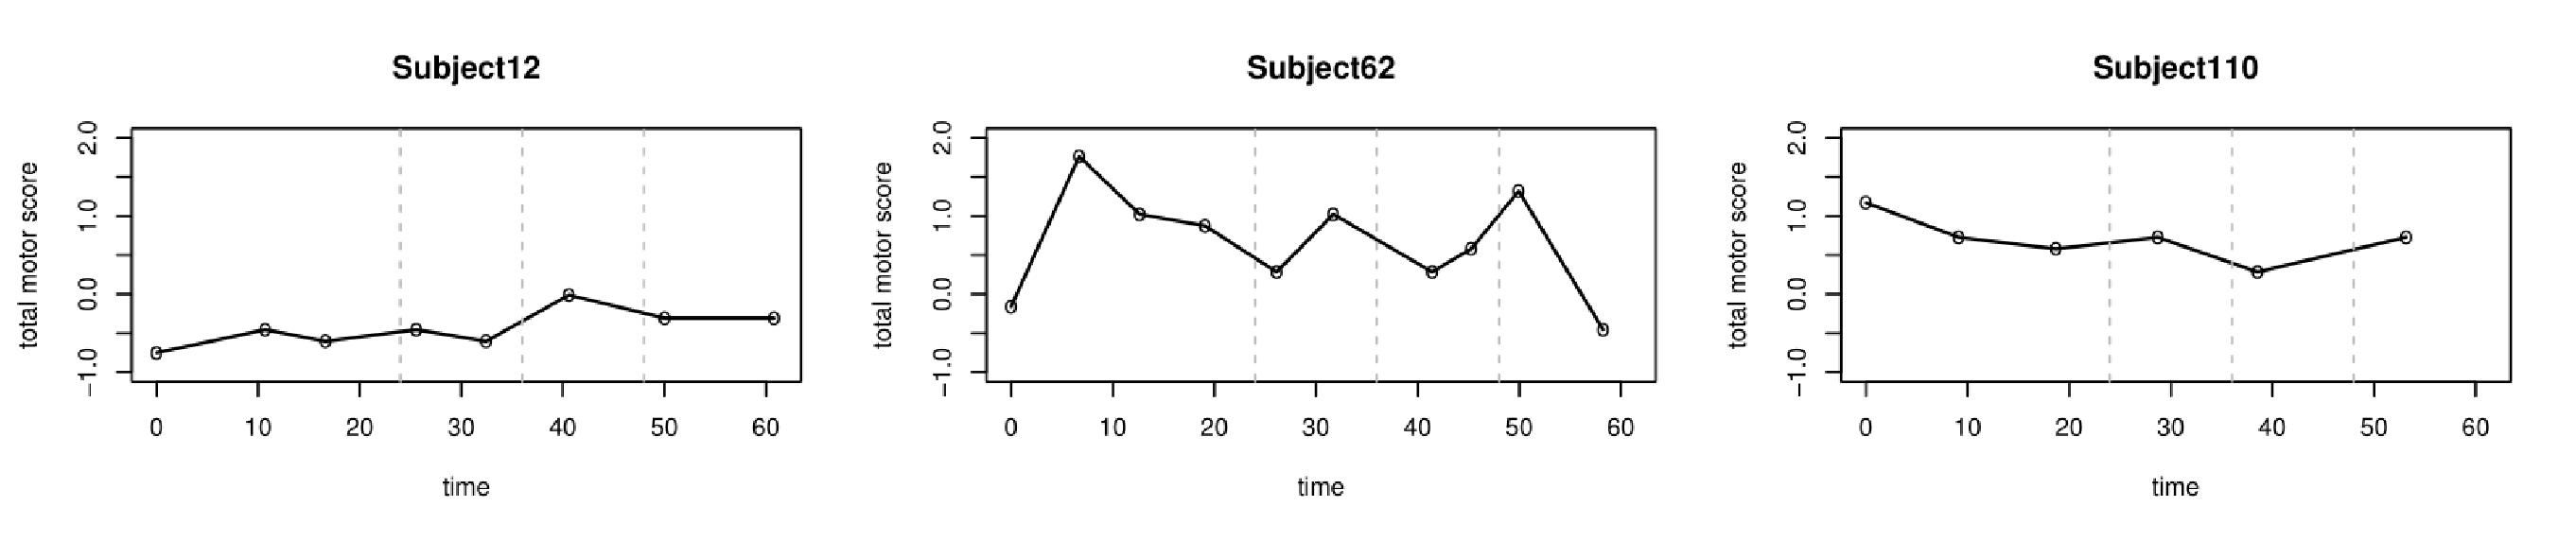
\includegraphics[width=\columnwidth]{test_long_plot_12_62_110.eps}\label{plot:datafig11}
}

% \centering
\subfloat[Predictions based on censoring time $t=$ 24 months]{
    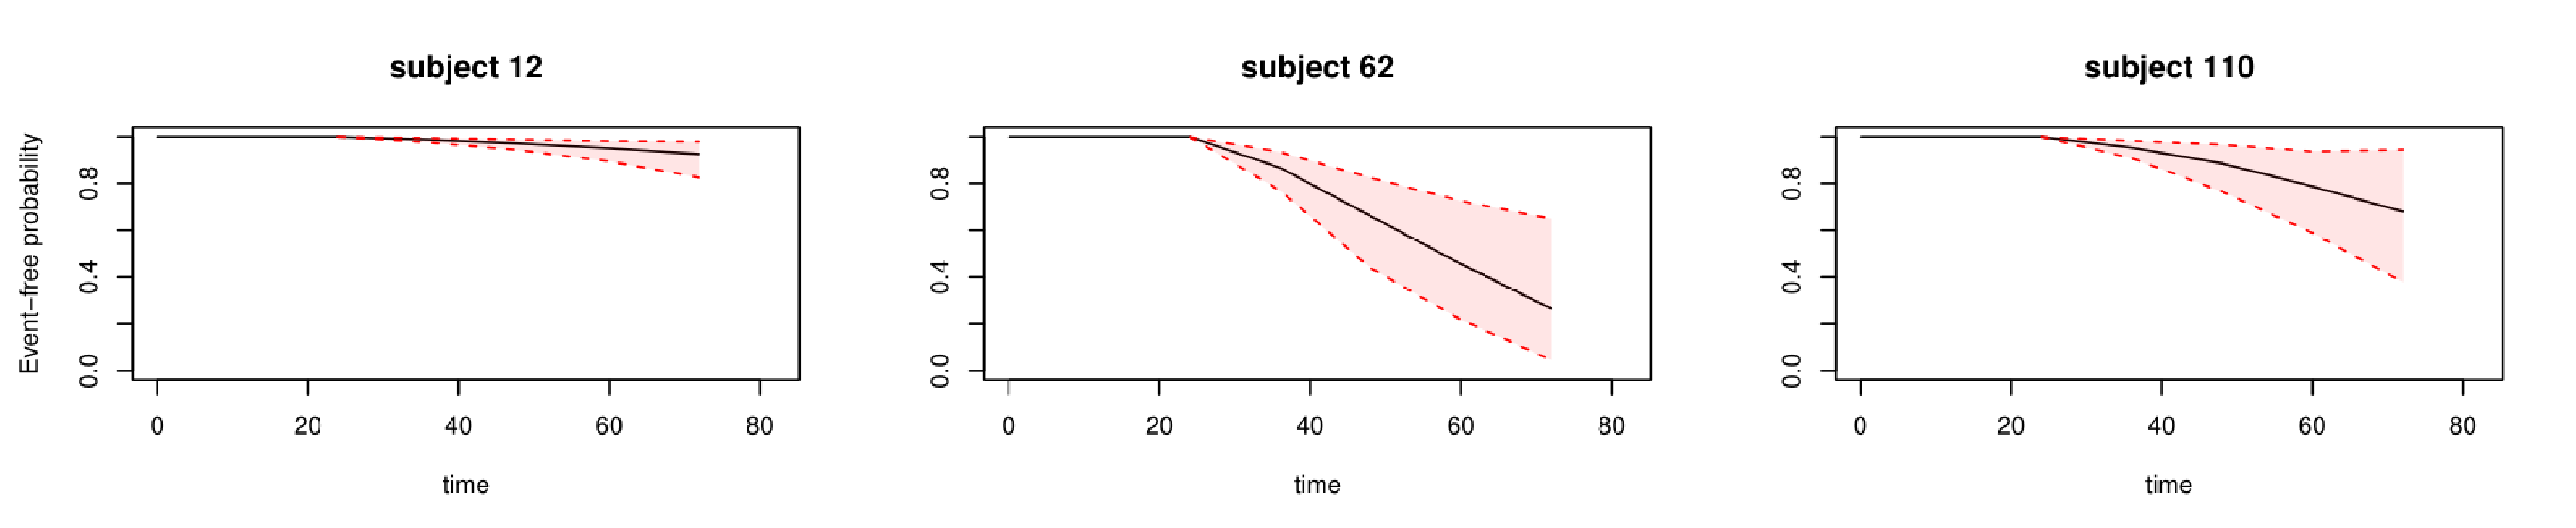
\includegraphics[width=\columnwidth]{neurotot_qt50_pred_surv_t24_id_12_62_110.eps}\label{plot:datafig12}
}

\subfloat[Predictions based on censoring time $t=$ 36 months]{
    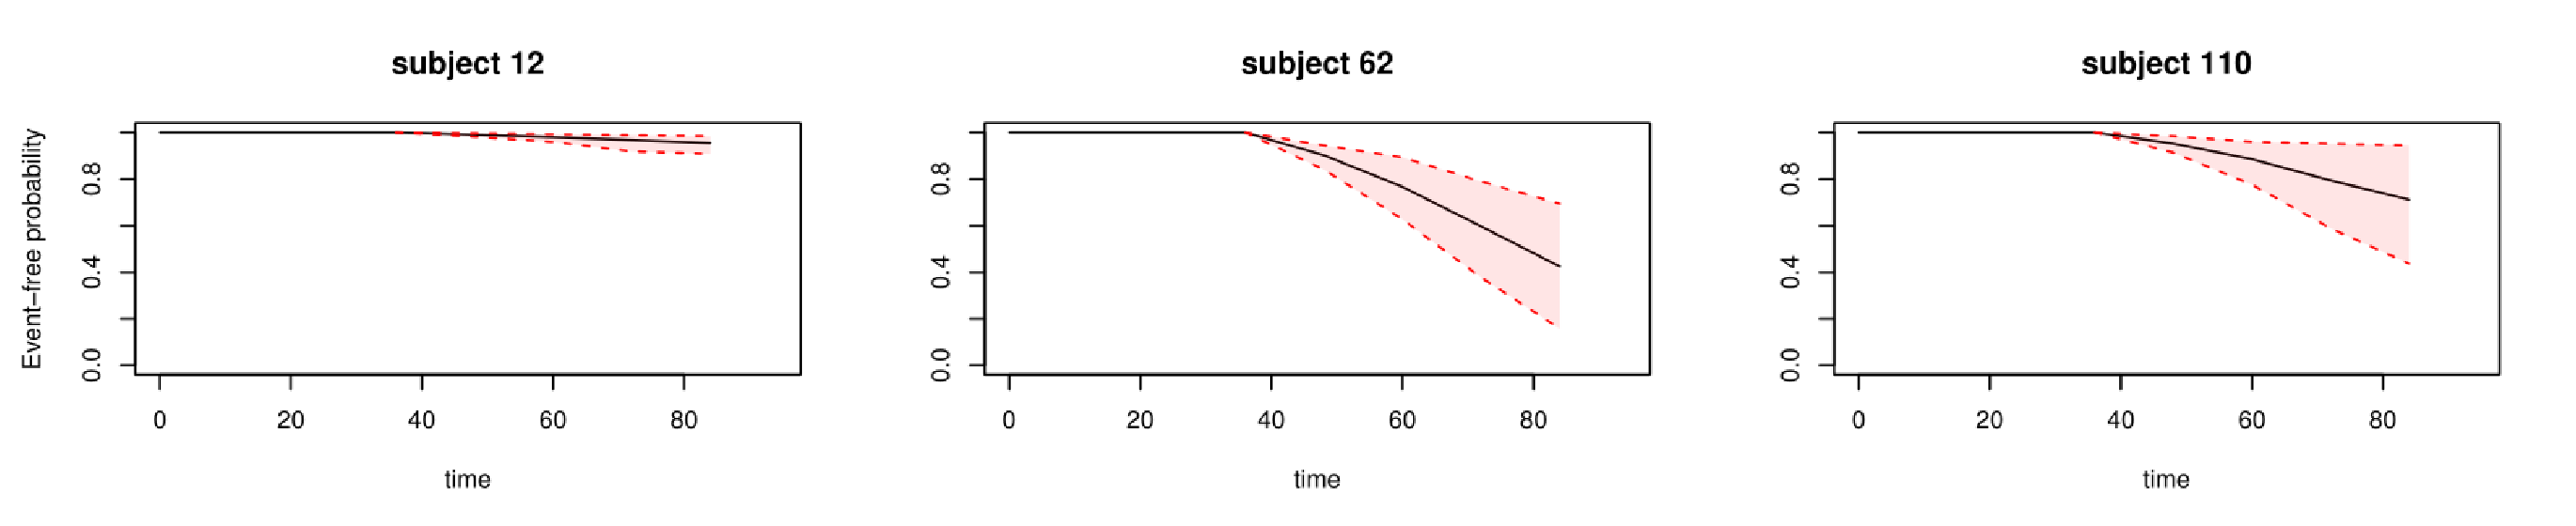
\includegraphics[width=\columnwidth]{neurotot_qt50_pred_surv_t36_id_12_62_110.eps}\label{plot:datafig13}
}

\subfloat[Predictions based on censoring time $t=$ 48 months]{
    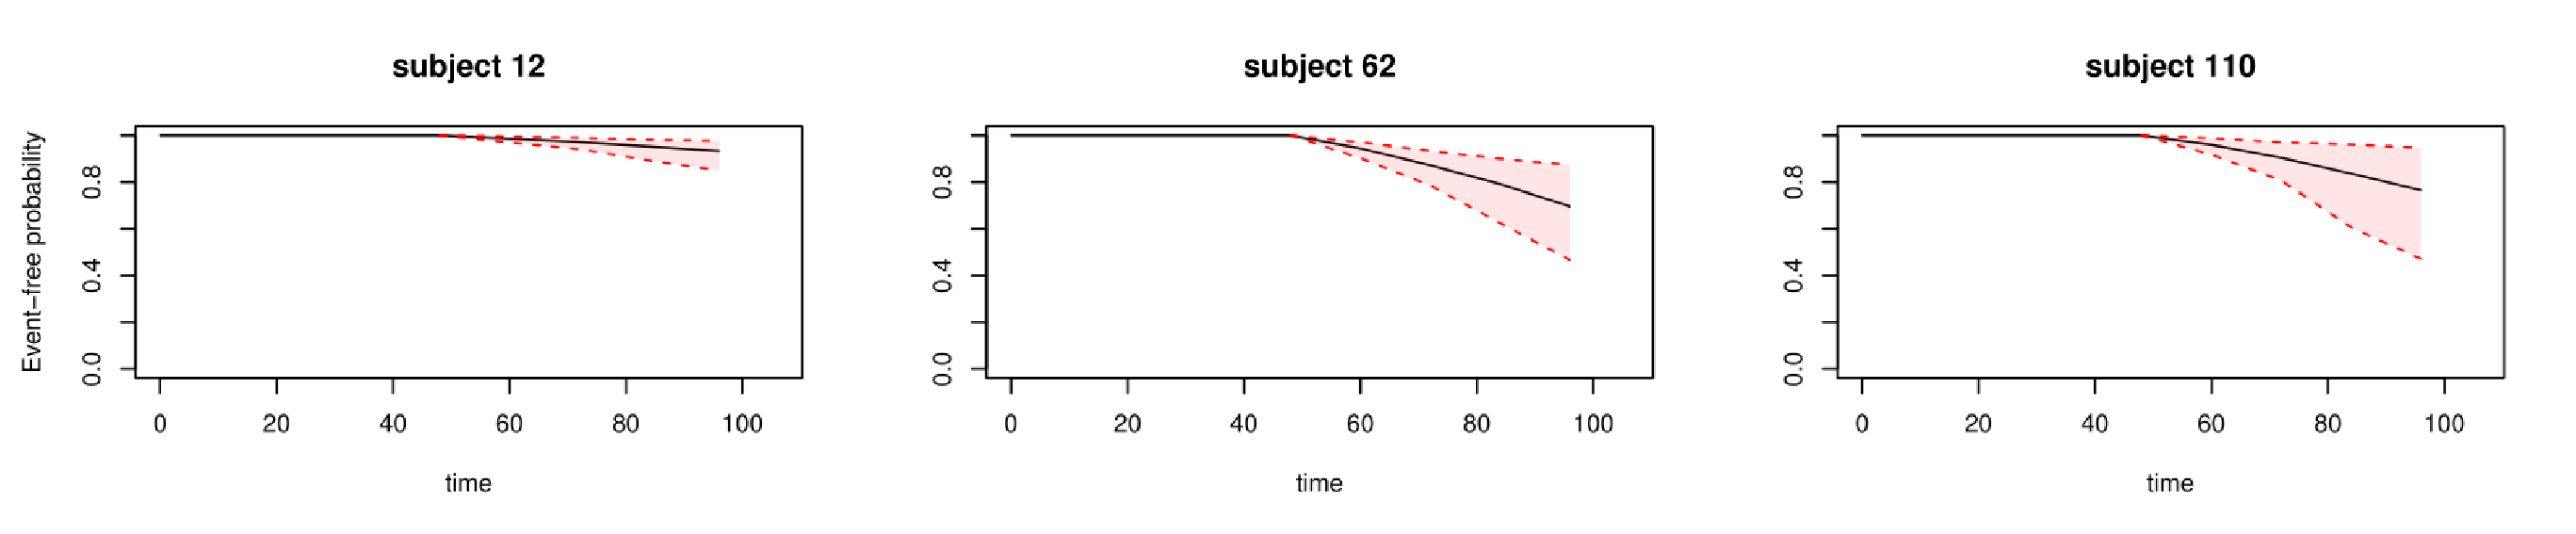
\includegraphics[width=\columnwidth]{neurotot_qt50_pred_surv_t48_id_12_62_110.eps}\label{plot:datafig14}
}

  \caption{PREDICT-HD data analysis: Longitudinal trajectories and dynamic predictions of HD-free probabilities with 95\% pointwise credible interval from QRJM at $\tau=0.5$ for selected subjects.}
  \label{plot:datafig1}
\end{figure}



% \end{document}

% \documentclass{article}
% \usepackage[utf8]{inputenc}
% \usepackage{fullpage}
% \usepackage {setspace}
% \usepackage[hang,flushmargin]{footmisc} %control footnote indent
% \usepackage{url} % for website links
% \usepackage{amssymb,amsmath}%for matrix
% \usepackage{graphicx}%for figure
% \usepackage{appendix}%for appendix
% \usepackage{float}
% \usepackage{multirow}
% \usepackage{longtable}
% \usepackage{morefloats}%in case there are too many float tables and figures
% \usepackage{caption}
% \usepackage{subcaption}
% \usepackage{listings}
% \captionsetup[subtable]{font=normal}
% \usepackage{color}
% \usepackage{hyperref}
% \usepackage[round]{natbib}
% \usepackage{appendix}
% \usepackage{listings}
% \usepackage{courier}
% \usepackage{color}


% \lstset{style=mystyle}


% \setlength{\parindent}{0em}
% \setlength{\parskip}{0.5em}


% \graphicspath{{0.plots/}}



% \begin{document}



\subsection{Discussion}\label{sec:discussion}
% What is done in this work, including data analysis part.
In our application of the LMJM (a linear mixed sub-model for the longitudinal process and a PH sub-model for the survival process) to Huntington's Disease, there are two limitations: first, the normality assumption of the random errors in the linear mixed model (LMM) was not realistic, and no obvious transformation of the longitudinal outcome to produce residual normality was applicable. This limitation is confirmed by our simulation studies where the LMJM tends to provide biased estimates to model parameters when the longitudinal data are non-normal. Consequently, predictive accuracy of the LMJM is negatively impacted. Second, the LMJM only models the conditional mean of the outcome. However, in our (and other) clinical research application(s), it may be more clinically relevant to consider the tails of the outcome distribution, e.g., the upper tail of TMS is at higher risk of developing HD.

Our proposed quantile regression joint models (QRJM) uses a linear quantile mixed model (LQMM) for the longitudinal process, improves both inference and the ability to make accurate dynamic predictions. The quantile-based estimators are more robust against skewness in the data, and as a result, our approach provides the flexibility to use median or quantile regression instead of mean regression when outliers and skewness are present in the longitudinal process. Moreover, the QRJM provides quantile-specific parameter estimates at a set of different quantiles and the researchers can choose the quantiles of interest and the corresponding inference results. The simulation studies and data application suggest that the QRJM not only inherits the good properties of an LMJM, but adds flexibility to the modeling procedure.

% Method summary and software.
% Limitation and
% Further work.
In this work, we develop a Bayesian algorithm to fit the proposed QRJM model and make dynamic predictions using the location-scale representation of the asymmetric Laplace distribution (ALD) for the longitudinal quantile regression. The Bayesian algorithm, which is straightforwardly implemented in \textsf{JAGS} software, uses a piecewise constant baseline hazard function in the survival sub-model. However, other functional forms can also be considered and the integration of the hazard function can be approximated using numerical integration such as Simpson's rule. In the real data application, we illustrate the flexibility of the QRJM and its advantages over the LMJM by jointly modeling the risk of developing HD and five commonly used early predictors of the disease. The QRJM is able to provide more insight into the disease progression and the association between the two disease processes in terms of various quantile-based estimations and dynamic predictions.

The novel application of our proposed QRJM in making personalized dynamic predictions of survival probability finds practical importance in many clinical applications. Event prediction using commonly collected biomarkers can provide clinicians with continuously updated ``disease progression'' information potentially allowing them to make appropriately timed intervention decisions for individual subjects. Subject-specific dynamic predictions models play an important role in the ongoing transformation of traditional medicine to patient-centric care. While in traditional medicine, treatments prescribed are guided by population-based experience, i.e., the average treatment effect in the entire population, such ``one-size-fits-all'' approaches are criticized for resulting in low efficacy and high adverse drug reactions in many clinical studies. Utilizing the dynamic predictions based on the proposed QRJM framework, we obtain subject-specific predictions of event risk that would actually allow physicians to target or tailor medical treatment based on a specific patient profile.

In summary, the QRJM is a good alternative to the LMJM when either the normality assumption of the errors term is concerned or the conditional quantiles are more relevant to research question. When the interest lies in the prediction of future survival probability, the ``best'' quantile may be chosen based on the predictive accuracy criteria. Other model selection methods or methods, e.g., Bayesian model averaging, to incorporate multiple regression results from different quantiles into a single prediction solution can be a potential direction for future work. However, in our opinion, the choice of specific quantile(s) should be more clinically oriented rather than be a statistical task.


% A question arises naturally from using quantile regression is which quantile should we choose? The answer is not unique and should depend on the specific research aim.

%All is done in \LaTeX \cite{knuth1986texbook}.
%
%
% \bibliographystyle{plainnat}%%%%%%%%%%%%%%%%%%%%
% \addcontentsline{toc}{section}{References}
% \bibliography{QRJM}


% \end{document}

% \newpage
% \documentclass[12pt]{article}
% \usepackage[text={7.1 in, 8 in}, top=1.75in, left=0.69in]{geometry}
% \usepackage[round]{natbib}
% \usepackage[utf8]{inputenc}
% \usepackage{fullpage}
% \usepackage {setspace}
% \usepackage[hang,flushmargin]{footmisc} %control footnote indent
% \usepackage{url} % for website links
% \usepackage{amssymb,amsmath}%for matrix
% \usepackage{graphicx}%for figure
% \usepackage{appendix}%for appendix
% \usepackage{float}
% \floatstyle{plaintop}
% \restylefloat{table}
% \usepackage{multirow}
% \usepackage{longtable}
% \usepackage{morefloats}%in case there are too many float tables and figures
% \usepackage{caption}
% % \usepackage{subcaption}
% \usepackage{subfig}
% \captionsetup[subtable]{font=normal}
% \usepackage{hyperref}
% \usepackage{courier}
% \usepackage{color}
% \usepackage{setspace}
% \usepackage{rotating} % rotate table by some degree
% \usepackage{rotfloat}
% \usepackage{mwe}
% \usepackage{listings}
% \usepackage{titling}
% \usepackage{lipsum}
% \usepackage[export]{adjustbox}




% \graphicspath{{figures/}}

% \begin{document}
% \author{\small{\bf Ming Yang, Sheng Luo,
% and Stacia M. DeSantis}\\
% \small{Department of Biostatistics, The University of Texas Health Science Center at Houston}}
% \date{}
% \title{\large{\bf Web-based Supplementary Material for ``Model Estimation and Dynamic Prediction in Joint Modeling Using Longitudinal Quantile Regression''}}
% \maketitle{}


\subsection*{Appendices}
\addcontentsline{toc}{subsection}{Appendices}
\renewcommand{\thesubsubsection}{\Alph{subsubsection}}

\subsubsection{Distribution Comparison}

\begin{itemize}
\item Laplace distribution (LD) with location at 0 and scale parameter equals 1 is symmetrical about 0. It has heavier tail compared with standard normal distribution.
\item Asymmetric Laplace distribution (ALD) is either positively or negatively skewed and the direction and degree of skewness are control by the skewness parameter $\tau \in [0,1]$.
\end{itemize}

\begin{figure}[H]
\centering
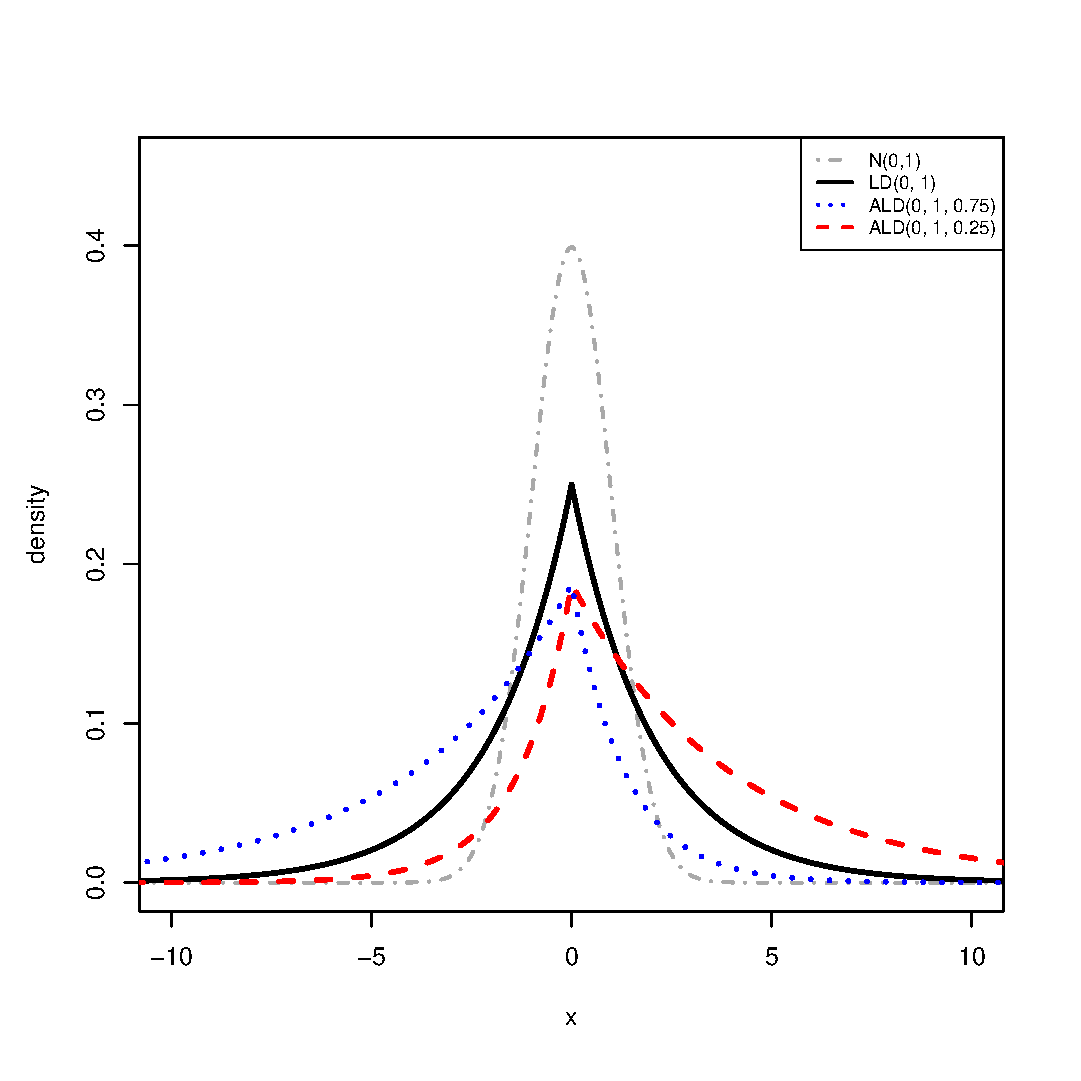
\includegraphics[width=0.6\columnwidth]{ald_ld_normal.eps}\label{plot:ald_ld_normal}
\caption{A comparison of normal, Laplace and asymmetric Laplace distributions.}
\end{figure}



\newpage
\subsubsection{Additional Simulation Results}\label{sec:appendix_simulation}

\begin{table}[H]
\centering
\caption{Simulation result in Simulation study I Scenario 2 in which random errors are generated from ALD with $\tau=0.5$.}
\adjustbox{max width=\textwidth}{
\label{tab:sim1tab2}
\begin{tabular}{lccccccccc}
\hline
& \multicolumn{4}{c}{QRJM ($\tau=0.5$)} & & \multicolumn{4}{c}{LMJM}\\
\hline
 & Bias & SE & MSE & CP & & Bias & SE & MSE & CP \\
\hline
  \multicolumn{10}{l}{Coefficients for longitudinal process} \\
  $\beta_0$ & $-$0.006 & 0.069 & 0.009 & 0.960 & & 0.013 & 0.093 & 0.017 & 0.960 \\
  $\beta_{1}$ & 0.008 & 0.060 & 0.008 & 0.900 & & 0.018 & 0.079 & 0.018 & 0.880 \\
  $\beta_{2}$ & 0.014 & 0.075 & 0.011 & 0.950 & & 0.031 & 0.093 & 0.021 & 0.940 \\
  \multicolumn{10}{l}{Coefficients for survival process} \\  
  $\gamma_1$ & 0.008 & 0.055 & 0.006 & 0.940 & & 0.014 & 0.058 & 0.007 & 0.950 \\
  $\gamma_2$ & 0.007 & 0.055 & 0.007 & 0.950 & & 0.013 & 0.057 & 0.007 & 0.950 \\
  $\alpha$ & $-$0.001 & 0.071 & 0.011 & 0.930 & & $-$0.028 & 0.101 & 0.086 & 0.920 \\
   \hline
\end{tabular}
}
\end{table}


% latex table generated in R 3.2.2 by xtable 1.7-4 package
% Tue Oct 27 23:07:31 2015
\begin{table}[H]
\centering
\caption{Simulation result in Simulation study I Scenario 3 in which random errors are generated from $\mathcal{N}(0, 1)$.}
\adjustbox{max width=\textwidth}{
\label{tab:sim1tab3}
\begin{tabular}{lccccccccc}
\hline
& \multicolumn{4}{c}{QRJM ($\tau=0.5$)} & & \multicolumn{4}{c}{LMJM} \\
\hline
 & Bias & SE & MSE & CP & & Bias & SE & MSE & CP \\
\hline
  \multicolumn{10}{l}{Coefficients for longitudinal process} \\

  $\beta_0$ & 0.015 & 0.037 & 0.003 & 0.950 & & 0.000 & 0.035 & 0.002 & 0.980 \\
  $\beta_{1}$ & 0.004 & 0.034 & 0.002 & 0.960 & & $-$0.003 & 0.033 & 0.002 & 0.950\\
  $\beta_{2}$ & 0.013 & 0.050 & 0.005 & 0.950 & & 0.006 & 0.049 & 0.005 & 0.950 \\
  \multicolumn{10}{l}{Coefficients for survival process} \\  
  $\gamma_1$ & 0.008 & 0.055 & 0.006 & 0.920 & & 0.003 & 0.054 & 0.006 & 0.900 \\
  $\gamma_2$ & 0.015 & 0.055 & 0.007 & 0.920 & & 0.010 & 0.054 & 0.006 & 0.920 \\
  $\alpha$ & $-$0.013 & 0.055 & 0.006 & 0.950 & & 0.007 & 0.055 & 0.006 & 0.950 \\
   \hline
\end{tabular}
}
\end{table}


\begin{table}[H]
\centering
\caption{Prediction results in Simulation study II Scenario 3 in which random errors are generated from ALD with $\tau=0.5$.}
\adjustbox{max width=\textwidth}{
\label{tab:sim2tab2}
\begin{tabular}{clccccc}
\hline
 & & \multicolumn{2}{c}{QRJM ($\tau=0.5$)} & &\multicolumn{2}{c}{LMJM}\\
\cline{3-4}\cline{6-7}
$t$ & $\Delta t$ & MSE & Bias & & MSE & Bias \\
\hline
\multirow{2}{*}{{\bf 0.25}} & 0.25 & 0.005 & 0.005 && 0.005 & $-$0.001 \\
&  1 & 0.009 & 0.005 &&  0.009 & 0.000 \\
\multirow{2}{*}{(subjects left: 47.87\%)} &  2 & 0.011 & 0.003 && 0.010 & 0.000 \\
&  3 & 0.011 & 0.002 && 0.011 & 0.001 \\
\hline
\multirow{2}{*}{{\bf 0.5}} & 0.25 & 0.004 & 0.005 && 0.003 & $-$0.002 \\
&   1 & 0.009 & 0.004 && 0.008 & $-$0.002 \\
\multirow{2}{*}{(subjects left: 34.78\%)}&   2 & 0.012 & 0.002 && 0.011 & $-$0.001 \\
&   3 & 0.013 & 0.001 && 0.012 & $-$0.001 \\
\hline
\multirow{2}{*}{{\bf 0.75}} & 0.25 & 0.002 & 0.004 && 0.002 & $-$0.002 \\
& 1 & 0.009 & 0.005 && 0.007 & $-$0.002 \\
\multirow{2}{*}{(subjects left: 27.71\%)} & 2 & 0.012 & 0.002 && 0.011 & $-$0.003 \\
&  3 & 0.014 & 0.001 && 0.012 & $-$0.002 \\
\hline
\end{tabular}
}
\end{table}


\begin{figure}[H]
\centering
\subfloat[][QRJM with $\tau=0.25$ (True model)]{
    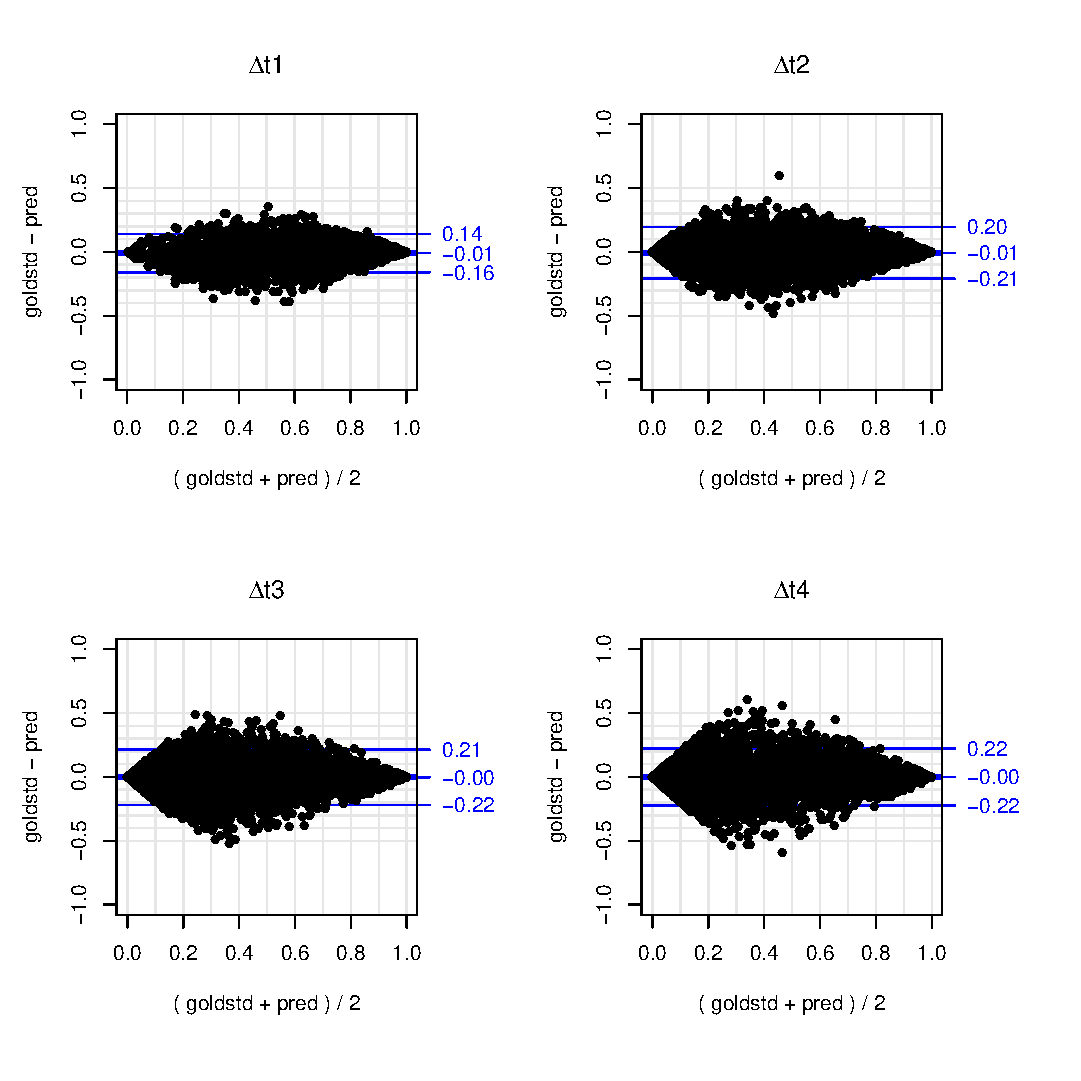
\includegraphics[width=0.45\columnwidth]{baplot_qt25data_qt25fit_t1.eps}\label{plot:sim2fig11}
}
% \centering
\subfloat[][QRJM with $\tau=0.5$]{
    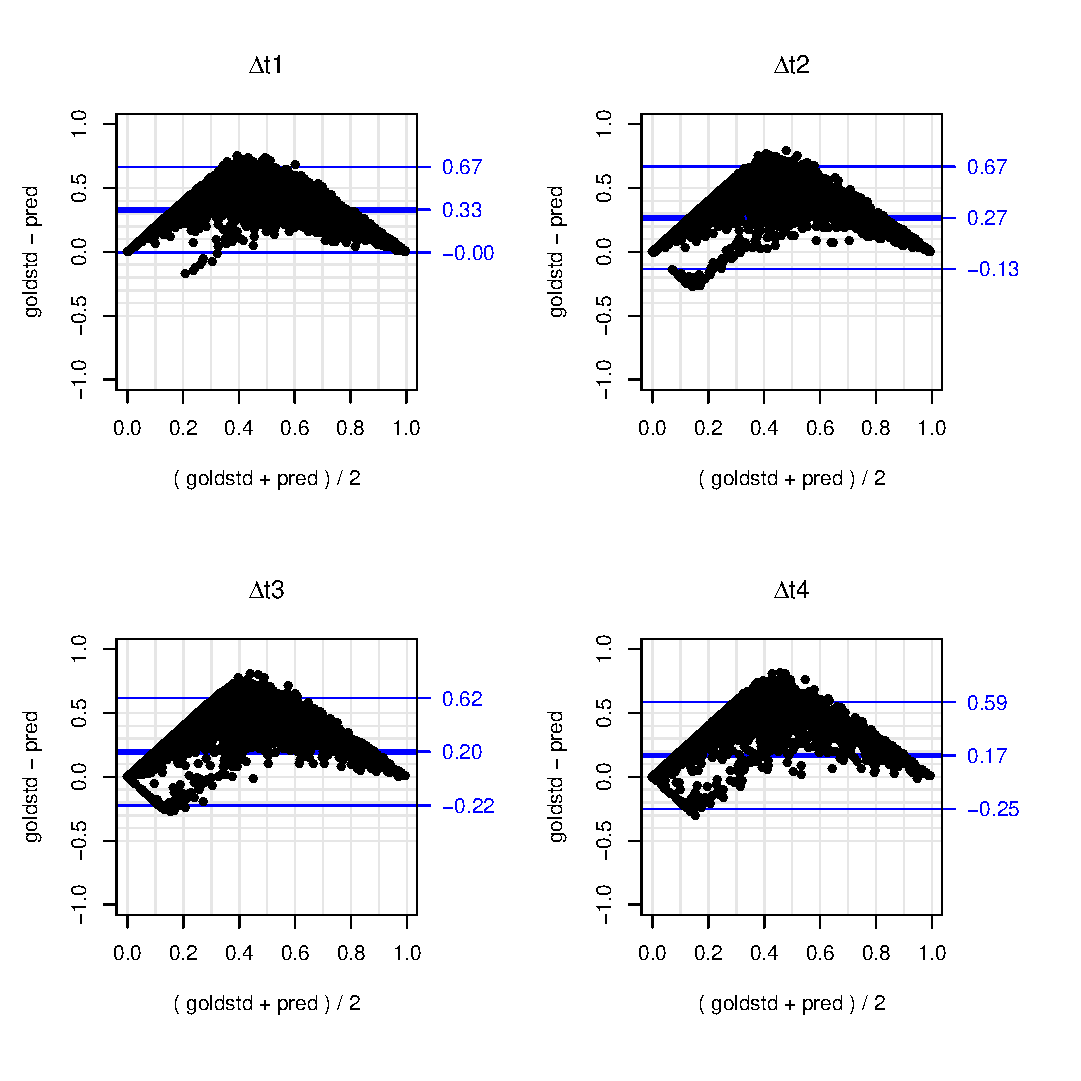
\includegraphics[width=0.45\columnwidth]{baplot_qt25data_qt50fit_t1.eps}\label{plot:sim2fig12}
}

\subfloat[][LMJM]{
    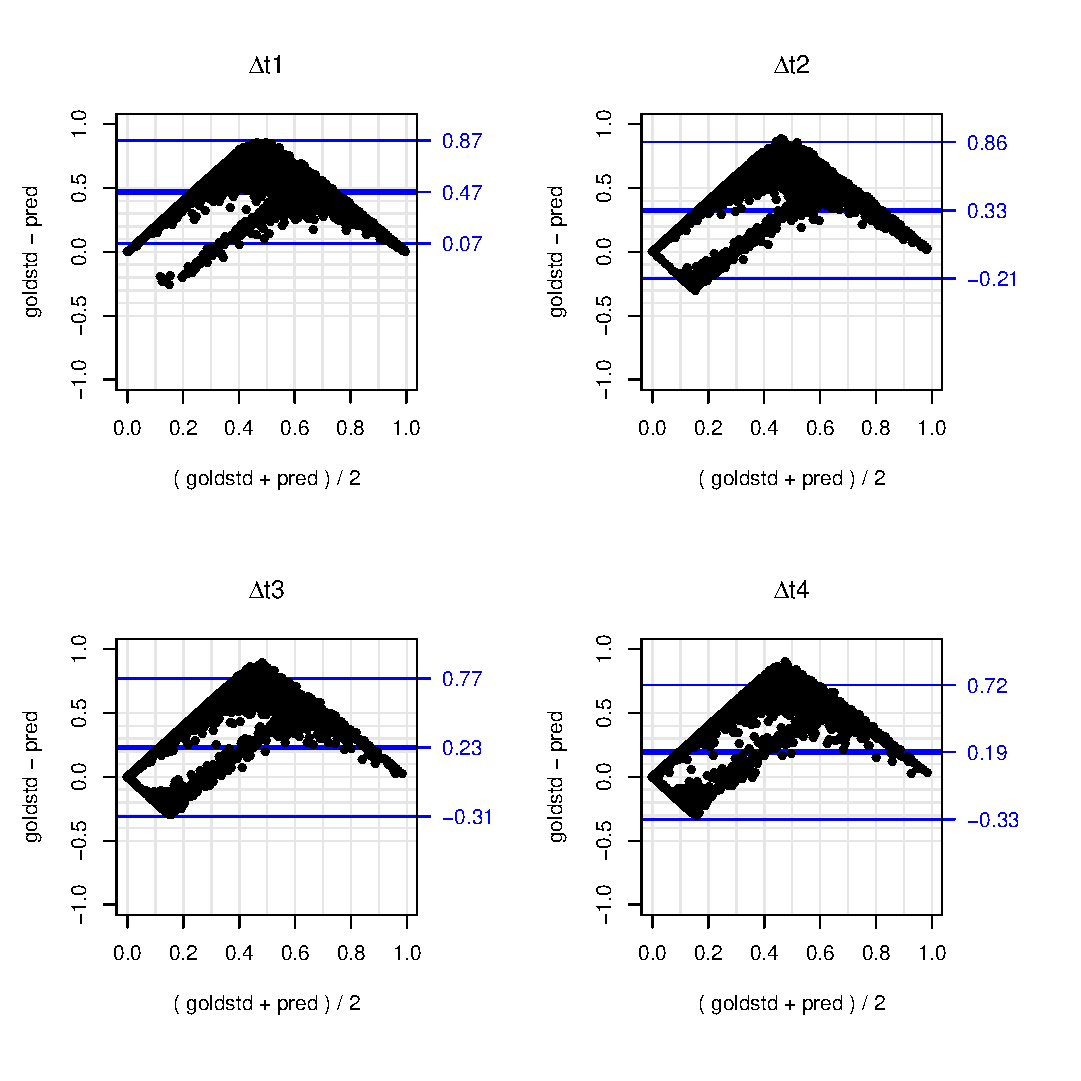
\includegraphics[width=0.45\columnwidth]{baplot_qt25data_LMJMfit_t1.eps}\label{plot:sim2fig13}
}
  \caption{Prediction results in Simulation study II Scenario 1: Bland-Altman plot (bias and 95\% limits of agreement) of gold standard versus model predictions at four prediction time intervals ($\Delta t_1 < \Delta t_2 < \Delta t_3 < \Delta t_4$).}
  \label{plot:sim2fig1}
\end{figure}

\begin{figure}[H]
\centering
\subfloat[][LMJM (True model)]{
    \includegraphics[width=0.45\columnwidth]{baplot_normdata_LMJMfit_arms_t1.pdf}\label{fig:3a}
}
% \centering
\subfloat[][QRJM with $\tau=0.5$]{
    \includegraphics[width=0.45\columnwidth]{baplot_normdata_qt50fit_arms_t1.pdf}\label{fig:3b}
}
  \caption{Prediction results in Simulation study II Scenario 3: Bland-Altman plot (bias and 95\% limits of agreement) of gold standard versus model predictions based on the first two longitudinal observations and four different prediction time intervals ($\Delta t_1 < \Delta t_2 < \Delta t_3 < \Delta t_4$).}
  \label{plot:sim2fig2}
\end{figure}



\subsubsection{Variable Definitions}\label{sec:appendix_var_description}
\begin{itemize}
\item {Total motor score}: Standardized ratings of oculomotor function, dysarthria, chorea, dystonia, gait and postural stability based on the Unified Huntington Disease Rating Scale (UHDRS).

\item {Putamen}: the volume of putamen, which a round structure located at the base of the forebrain. The atrophy of the putamen is related with impaired movements regulation and learning ability.

\item {Stroop word}: Stroop Color and Word Test score. The test consists of three 45-second trials, including two trials measure basic attention and process speed and a third trail tests the ability to identifying the name of a color (e.g., ``blue'', ``green'', or ``red'') that is printed in a color not denoted by the name.

\item {FrBe executive subscale}: Frontal System Behavioral Scale -- executive subscale -- companion rating scale. Part of a 46-item behavior rating scale on abstraction, problem solving, and hypothesis generation as rated by a companion focusing on dorsolateral prefrontal circuitry.

\item {Total functional capacity}: A list of independent and common daily tasks that can be accomplished bas on the UHDRS.

\end{itemize}



\subsubsection{LOESS Plots of Selected Longitudinal Variables}

\begin{figure}[H]
\centering
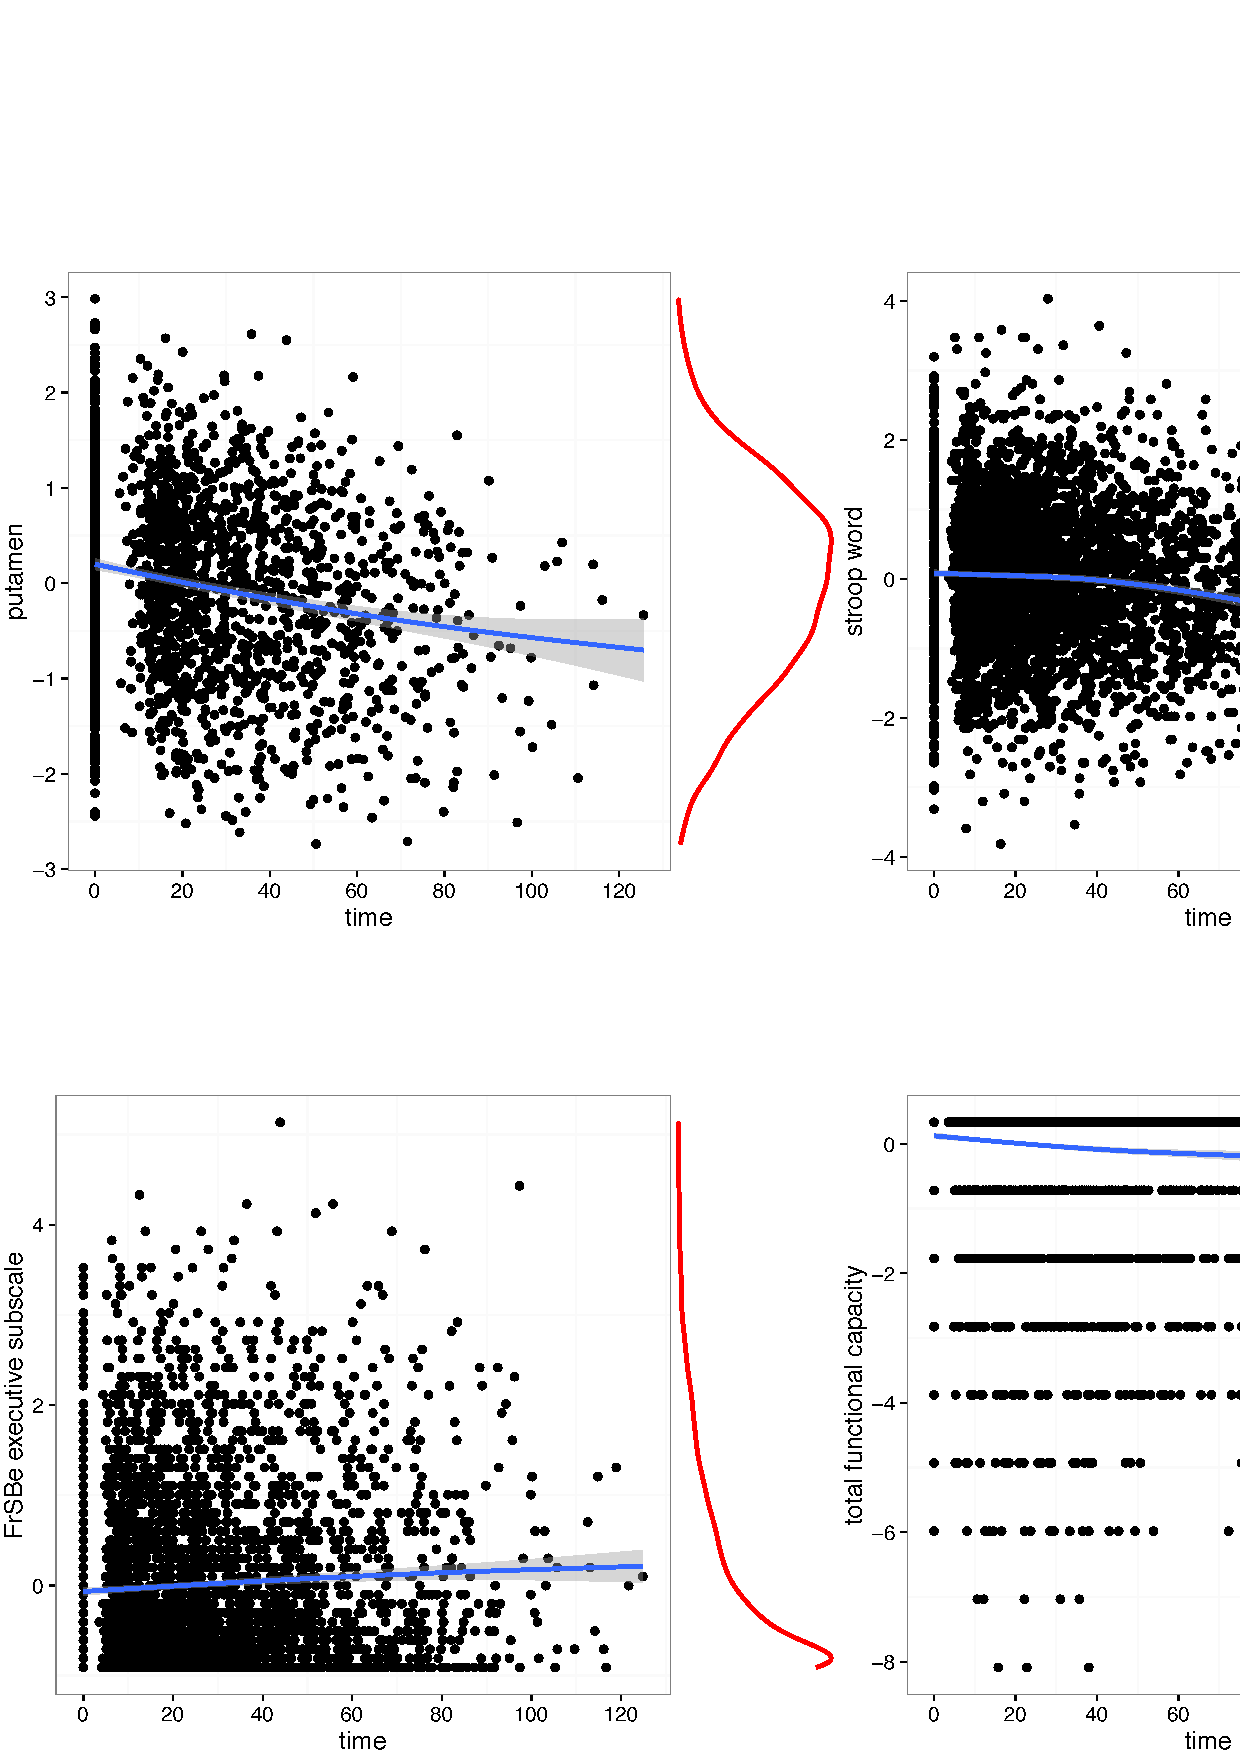
\includegraphics[width=1.0\linewidth]{data_densities_loess.pdf}
\caption{Scatter plot with LOESS curve for {putamen (top left)}, {stroop word (top right)}, {FrBe executive subscale (bottom left)} and {total functional capacity (bottom right)} from the study population.}
\label{fig:data_densities}
\end{figure}

\singlespacing
\section{Additional Data Analysis Results}\label{sec:appendix_realdata}
\begin{table}[H]
\centering
\caption{PREDICT-HD data analysis: Parameter estimation and 95\% credible interval (in parenthesis) from QRJM at three quantiles (0.25, 0.5, and 0.75) with putamen, stroop word, FrBe executive subscale (FES), and total functional capacity (TFC) being the longitudinal biomarkers.}
\label{realdata_inference}
\resizebox{\linewidth}{!}{
\begin{tabular}{l ccc r ccc}
  \hline
  & \multicolumn{3}{c}{{putamen}}&& \multicolumn{3}{c}{{stroop word}}\\
  \hline
  & $\tau=0.25$ & $\tau=0.50$ & $\tau=0.75$ & & $\tau=0.25$ & $\tau=0.50$ & $\tau=0.75$\\
\hline
\multicolumn{8}{l}{For longitudinal process} \\
int. & 1.045 & 1.142  & 0.1.243 && 0.123  & 0.370 & 0.625 \\
  &(0.830, 1.266)& (0.864, 1.439) & (1.003, 1.511) && (-0.136, 0.378) & (0.114, 0.640) & (0.382, 0.857) \\

time (month) & -0.014 & -0.014  & -0.014 && -0.007 & -0.007 & -0.007\\
  & (-0.018, -0.010) & (-0.017, -0.010) & (-0.017, -0.010) && (-0.010, -0.004) & (-0.010, -0.003) & (-0.010, -0.004)\\

$age_0$ & -0.023 & -0.023  & -0.017 && -0.006 & -0.007 & -0.007 \\
  & (-0.028, -0.018) & (-0.030, -0.017) & (-0.029, -0.017) && (-0.013, 0.000) & (-0.013, 0.000) & (-0.013, -0.001)\\ \\

\multicolumn{8}{l}{For time to HD onset process} \\
assoct. & -1.038 & -1.039  & -1.045 && -0.696 & -0.709 & -0.719 \\
  & (-1.213, -0.861)& (-1.217, -0.860) & (-1.224, -0.862) && (-0.832, -0.558) & (-0.846, -0.573) & (-0.853, -0.581) \\

eduyr & -0.060 & -0.055  &  -0.050 && -0.080 & -0.069 & -0.059  \\
  & (-0.094, -0.027)& (-0.093, -0.021) & (-0.090, -0.015) && (-0.106, -0.053) & (-0.097, -0.043) & (-0.088, -0.032)\\

male & -0.021 & -0.020 & -0.017 && -0.173 & -0.166 & -0.157 \\
  & (-0.347, 0.283)& (-0.336, 0.290) & (-0.330, 0.303) && (-0.459, 0.111) & (-0.458, 0.111) & (-0.449, 0.124) \\
  \hline
  \hline
  & \multicolumn{3}{c}{{FrBe executive subscale}}&& \multicolumn{3}{c}{{total functional capacity}}\\
  \hline
  & $\tau=0.25$ & $\tau=0.50$ & $\tau=0.75$ & & $\tau=0.25$ & $\tau=0.50$ & $\tau=0.75$ \\
\hline
\multicolumn{8}{l}{For longitudinal process}\\
int. & -0.533 & -0.244 & 0.138 && 0.277  & 0.333 & 0.362  \\
  & (-0.731, -0.328) & (-0.493, -0.021) & (0.261, 0.494) && (0.218, 0.355) & (0.293, 0.372) &  (0.330, 0.394)\\

time (month) & 0.007 & 0.006 & 0.006 && -0.028 & -0.016 & -0.007 \\
  & (0.003, 0.011) & (0.003, 0.010) & (0.002, 0.010) && (-0.033, -0.024) & (-0.020, -0.012) &  (-0.012, -0.004)\\

$age_0$ & 0.002 & 0.002 & 0.001 && -0.001  & -0.000 & 0.000 \\
  & (-0.003, 0.007) & (-0.003, 0.008) & (-0.006, 0.008) && (-0.002, 0.001) & (-0.001, -0.001) &  (-0.001, 0.001)\\\\

\multicolumn{8}{l}{For time to HD onset process}\\
assoct. &  0.524 & 0.434 & 0.376 && -0.374 & -0.478 &  -0.488\\
  & (0.378, 0.667) & (0.306, 0.435) & (0.261, 0.494) && (-0.438,-0.305) & (-0.569, -0.389) &  (-0.596, -0.378)\\

eduyr & -0.077 & -0.082 & -0.091 && -0.097 & -0.093 &  -0.093 \\
  & (-0.116, -0.041) & (-0.119, -0.052) & (-0.125, -0.060) && (-0.135, -0.064) & (-0.134, -0.058) &  (-0.138, -0.054) \\

male & -0.263 & -0.301 & -0.291 && 0.104 & 0.057 & 0.031 \\
  & (-0.560, 0.051) & (-0.611, 0.004) & (-0.602, 0.006) && (-0.207, 0.405) & (-0.260, 0.354) &  (-0.286, 0.329) \\
  \hline
\end{tabular}
}
\end{table}


\doublespacing
\newpage
\subsubsection{\textsf{JAGS} Model File}\label{p1:jags_code}
\textsf{JAGS} model file to fit QRJM in simulation study.
{\scriptsize
\begin{verbatim}
model{
      k1 <- (1-2*qt)/(qt*(1-qt))
      k2 <- 2/(qt*(1-qt))
      for (i in 1:I){
        # prior for random effects
        u[i, 1:2] ~ dmnorm(zero[], precision[,])
        # longitudinal process
        for (j in 1:J[i]){
            er[i,j] ~ dexp(sigma)
            mu[i,j] <- beta + u[i,1] + u[i,2]*t[j] + time[1]*X[i,1]
                    + time[2]*X[i,2]*t[j] + k1*er[i,j]
            prec[i,j] <- sigma/(k2*er[i,j])
            y[i,j] ~ dnorm(mu[i,j], prec[i,j])
        } #end of j loop
        # time-to-event process
        A[i] <- assoct.*u[i,2] + assoct.*time[2]*X[i,2]
        B[i] <- assoct.*(time[1]*X[i,1] + u[i,1] + beta) + inprod(gamma, W[i,])
        S[i] <- exp(-c*exp(B[i])*(exp(A[i]*Ti[i])-1)/A[i])
        h[i] <- c*exp(inprod(gamma, W[i,]) + assoct.*(beta +
            time[1]*X[i,1] + time[2]*X[i,2]*Ti[i] + u[i,1] + u[i,2]*Ti[i]))
        L[i] <- pow(h[i], event[i])*S[i]/1E+08
        phi[i] <- -log(L[i])
        zeros[i] ~ dpois(phi[i])
    }#end of i loop
    precision[1:2, 1:2] ~ dwish(Omega[,], 3)
    Sigma[1:2,1:2] <- inverse(precision[,])
    Omega[1,1] <- 1
    Omega[2,2] <- 1
    Omega[1,2] <- 0
    Omega[2,1] <- 0
    # priors for other parameters
    assoct. ~ dnorm(0, 0.001)
    int. ~ dnorm(0, 0.001)
    time[1] ~ dnorm(0, 0.001)
    time[2] ~ dnorm(0, 0.001)
    gamma[1] ~ dnorm(0, 0.001)
    gamma[2] ~ dnorm(0, 0.001)
    sigma ~ dgamma(0.001, 0.001)
    c ~ dunif(0.01, 10)
}
\end{verbatim}
}

\addcontentsline{toc}{subsection}{References}
\putbib[paper1]
\end{bibunit}

%%%%%%%%%% Journal article two %%%%%%%%%%%%%%%%%%%%%%%%%%%%
\newpage
\section{Journal Article 2}

{\bf Title of Journal Article}\\
Bayesian Quantile Regression Joint Models of Longitudinal and Recurrent Event Data

{\bf Journal proposed for article submission: Statistical Methods in Medical Research} \\

\newpage

\title{Bayesian Quantile Regression Joint Models of Longitudinal and Recurrent Event Data}
% \end{center}

\author{}
\date{}

\maketitle


\begin{center}
{\bf Abstract}
\end{center}

Recurrent event (e.g. heart failure, cancer recurrence, hospital readmissions, etc.) outcome is commonly encountered in longitudinal biomedical studies. In those studies, recurrent event outcome can be an important outcome of interest in monitoring disease progression or health condition of the study participants in addition to some continuous longitudinal outcome. For example, in the Atherosclerosis Risk In Communities Study (ARIC), which aims to investigate the causes of atherosclerosis and its clinical outcomes, and variation in cardiovascular risk factors, repeated systolic blood pressure (SBP) were measured at regular clinical visits for study participants. Meanwhile, recurrent event outcomes, including coronary heart disease, stroke, and heart failure, etc., were collected from extensive cohort surveillance. Previous studies using ARIC data revealed that there was a positive correlation between SBP and recurrent CHD events in the study cohort. This motivates us to consider the joint models (JM) of longitudinal and recurrent event data. JM models the bivariate outcomes jointly in accounting for the correlation between them, while studying potential disease risk factors for both outcomes simultaneously. In the traditional JM framework, a linear mixed model (LMM) is commonly used for the longitudinal outcome. LMM assumes normal random error; however, in many circumstances, the normality assumption cannot be satisfied and the it is not appropriate to use directly. Moreover, LMM only models the conditional mean of the longitudinal outcome, which may not be desirable in many clinical studies. In contrast to mean regression, quantile regression (QR) provides a more flexible, distribution-free way to study covariate effects at different quantiles of the longitudinal outcome. This becomes extremely important when higher (e.g. SBP) or lower (e.g. CD4 count) tail of the outcome is more relevant to clinical interest. In this paper, we propose to use the so-called linear quantile mixed model (LQMM) for the longitudinal outcome jointly with a proportional hazard model (PHM) for the recurrent event outcome under the JM framework. We develop a Gibbs sampler algorithm for the model inference, which is based on the location-scale representation of the asymmetric Laplace distribution for LQMM. We assess the performance of our Bayesian algorithm through extensive simulation study and applied the proposed model to the longitudinal SBP and recurrent CHD event data from the ARIC Study.

{\bf Key words:} Bayesian; Joint models; Linear quantile mixed model; Recurrent event.


\begin{bibunit}[apa]
% \documentclass{article}
% \usepackage[top=1.25in, bottom=1.1in, left=1.25in, right=1in]{geometry}
% \usepackage[utf8]{inputenc}
% \usepackage{fullpage}
% \usepackage {setspace}
% \usepackage[hang,flushmargin]{footmisc} %control footnote indent
% \usepackage{url} % for website links
% \usepackage{amssymb,amsmath}%for matrix
% \usepackage{graphicx}%for figure
% \usepackage{appendix}%for appendix
% \usepackage{float}
% \usepackage{multirow}
% \usepackage{longtable}
% \usepackage{morefloats}%in case there are too many float tables and figures
% \usepackage{caption}
% \usepackage{subcaption}
% \usepackage{listings}
% \captionsetup[subtable]{font=normal}
% \usepackage{color}
% \usepackage{hyperref}
% \usepackage[round]{natbib}

% %\usepackage{Sweave}
% \setlength{\parindent}{0em}
% \setlength{\parskip}{0.5em}


% \graphicspath{{0.plots/}}



% \begin{document}


\subsection{Introduction}

% JM in one or two sentences then talk about only the longitudinal part. Talk about the motivating data before introducing QR.

% Medical background of longitudinal and recurrent event data. Introduce the JM in analyzing these two types of data jointly.
In traditional joint models (JM) of longitudinal and time-to-event data, a linear mixed model (LMM) \citep{laird1982random} is commonly used for the longitudinal continuous outcome; while possible violation to the normality assumption in the error term is not considered. Moreover, an LMM only models covariate effects on the conditional mean of the outcome; however, in many clinical settings it is more desirable to make inference at lower or higher quantiles of the outcome. For example, researchers used quantile regression (QR) to study the risk factors of lower birth weight, in which they found several effects on the lower quantiles were significantly different from the mean effects \citep{koenker2001quantile}. In contrast to linear regression, QR is a more flexible tool that relaxes the distributional assumption, and provides a way to study covariate effects on various conditional quantiles of the outcome \citep{koenker2005quantile}. So far, there is little work has been done to connect QR method with the JM framework. To our knowledge, \cite{farcomeni2015longitudinal} is the first one to incorporate a linear quantile mixed model (LQMM) into a JM of longitudinal and terminal event data, in which they developed a Monte Carlo Expectation Maximization (MCEM) algorithm for parameter estimation.


Joint analysis of longitudinal and time-to-event outcomes have been studied by many authors. However, majority of the literature focuses on JM of longitudinal and a single time-to-event (e.g. death) data. For example, \cite{self1992modeling, tsiatis1995modeling, wulfsohn1997joint} developed the JM methods for survival analysis with a time dependent covariate measured with error. \cite{tsiatis2004joint} gives an excellent review of such JM method. In contrast, joint analysis of longitudinal and recurrent event outcomes has received less attention so far. To our knowledge, \cite{henderson2000joint} developed a shared random effects JM for longitudinal data and recurrent events. \cite{kim2012joint} considered a JM of longitudinal and recurrent event data with informative terminal event. \cite{efendi2013joint} proposed a JM of longitudinal and recurrent event outcomes that accommodates overdispersion. Furthermore, there is little work has consider using LQMM in the JM of longitudinal and recurrent event data.

% Recurrent events, such as multiple cardiovascular diseases (CVD), cancer recurrences, and hospital readmissions, are commonly encountered in clinical studies. Meanwhile, during the follow-up, some longitudinal outcomes are usually measured repeatedly at regular clinical visits or when events occur. It is common that longitudinal biomarkers are informative for the occurrence of repeated events in many clinical settings. As a typical example, patients with higher blood pressure (BP) are more likely to experience coronary heart diseases (CHD) \citep{wattanakit2005risk, rodriguez2014systolic}. Ignoring the dependence between the longitudinal and recurrent event processes and the fit models for the two outcomes separately will lead to loss of information and result in biased or inefficient inference results. Traditional survival model with time-varying covariate may not be appropriate to use due to its limiting assumption of external time-dependent covariates that are not related to the event mechanism. In contrast, joint models (JM) of longitudinal and recurrent event data is more appropriate to use to study the association between the two processes and to model the two outcomes simultaneously.

In this paper, we propose a new version of JM for longitudinal and recurrent event data, in which we adopt the LQMM in modeling the longitudinal continuous outcome and use the Cox proportional hazards model (PHM) for recurrent events. The model takes the format of shared random effects JM, similar as in \cite{wulfsohn1997joint} and \cite{rizopoulos2011dynamic}, in which the longitudinal outcome is treated as a time-dependent covariate in the recurrent event model and the dependence is measured by some association parameter. We develop a Gibbs sampling algorithm for model inference, which is based on the fact that minimizing the original QR loss function is equivalent to maximizing the likelihood function of the so-called asymmetric Laplace distribution (ALD) \citep{yu2001bayesian}. Moreover, the ALD can be further reparameterized using a location-scale mixture representation that leads to a combination of normal and exponential distributions \citep{kotz2001laplace, kozumi2011gibbs,luo2012bayesian}. The proposed Bayesian estimating algorithm can be directly implemented in existing software. In application, we use the data from the Atherosclerosis Risk in Communities Study (ARIC) \citep{aric1989atherosclerosis}, in which we investigate various covariate effects on different quantiles of the systolic blood pressure (SBP) and its association with the recurrences of coronary heart disease (CHD). QR based JM is able to add much more flexibility in modeling and provide additional insight into the data by investigating covariate effects on various conditional quantiles of SBP and its association with the risk of CHD recurrence, which are not possible using traditional mean regression based methods.



% This feature find its great importance in biomedical studies, where individuals with extremer biomarker measurements are often at higher risk of disease or death.


%paper organization
The rest of this paper is organized as follows. In Section \ref{sec:p2methods}, we give details of the proposed statistical model and the Bayesian algorithm for model inference. In Section \ref{sec:p2simulation}, we present simulation study to validate the proposed methods. In Section \ref{sec:p2data}, we apply the proposed methods to the ARIC data. We conclude the paper with a discussion in Section \ref{sec:p2discussion}.
% \bibliographystyle{plainnat}%%%%%%%%%%%%%%%%%%%%
% \addcontentsline{toc}{section}{References}
% \bibliography{QRJM}
% \end{document}




\subsection{Methods}\label{sec:p2methods}
% reformat the subsection section since it was changed in the appendix part of paper 1
\renewcommand{\thesubsubsection}{\thesubsection.\arabic{subsubsection}}
%%%%%%%%%%%%%%%%%%%%%%%%%%%
\subsubsection{Bayesian Linear Quantile Mixed Model}\label{sec:p2BLQMM}
Let $Y_{i}(t_{ij})$ be the longitudinal outcome for subject $i$ measured at time $t_{ij}$ where $i=1, \cdots, N\mbox{ and } j=1,\cdots, n_i$. Consider the linear mixed effects model:
\begin{equation}\label{eqn:p2lmm}
Y_{i}(t) ={\boldsymbol X}_{i}^{\top}(t) \boldsymbol{\beta}+ {\boldsymbol Z}_{i}^{\top}(t)\boldsymbol{u}_i + \varepsilon_{i}(t),
\end{equation}

\noindent where $\boldsymbol{\beta}$ is a $p-$dimensional vector of fixed effects,  ${\boldsymbol X}_{i}(t)$ contains the corresponding fixed covariates, $\boldsymbol{u}_i$ is a $k-$dimensional vector of random effects for subject $i$, and ${\boldsymbol Z}_{i}(t)$ are the corresponding random covariates.

An LQMM assumes that the conditional quantile of the outcome is a linear function of the covariates, i.e.,
\begin{equation}\label{eqn:p2lqmm}
Q_{Y_{i}(t)|{\boldsymbol X}_{i}(t),{\boldsymbol Z}_{i}(t)}(\tau)={\boldsymbol X}_{i}^{\top}(t) \boldsymbol{\beta}+ {\boldsymbol Z}_{i}^{\top}(t)\boldsymbol{u}_i,
\end{equation}

\noindent where the $\tau$th quantile of a random variable $Y$ is defined as $Q_{Y}(\tau)=F_{Y}^{-1}(\tau)=\inf\left\{ y:F_{Y}(y)\geq\tau\right\}$, for $\tau\in [0, 1]$. Parameter estimations can then be obtained by minimizing the following loss function,

\begin{equation*}\label{eqn:p2loss_fun}
\hat{\boldsymbol{\beta}}_{\tau}=\underset{\boldsymbol{\beta}\in \mathbb{R}^{p}}{\mbox{arg min}}\sum_{i, t}\left[\rho_{\tau}\left(Y_{i}(t)-{\boldsymbol X}_{i}^{\top}(t)\boldsymbol{\beta} - {\boldsymbol Z}_{i}^{\top}(t)\boldsymbol{u}_i\right)\right],
\end{equation*}

\noindent where $\rho_{\tau}(\cdot)$ is defined as $\rho_{\tau}(Y)=Y(\tau-{I}{(Y<0)}).$

Above minimization problem can be rephrased as a maximum-likelihood problem by assuming the random error $\varepsilon_{i}(t)$ in (\ref{eqn:p2lmm}) follows ALD with location parameter equals 0, scale parameter $\sigma$ and skewness parameter $\tau$ \citep{koenker1999goodness,yu2001bayesian}:
\begin{equation*}
Y_{i}(t) ={\boldsymbol X}_{i}^{\top}(t) \boldsymbol{\beta}+ {\boldsymbol Z}_{i}^{\top}(t)\boldsymbol{u}_i + \varepsilon_{i}(t), \varepsilon_{i}(t)\sim ALD(0, \sigma, \tau).
\end{equation*}

This becomes clear when writing out the conditional likelihood function:
\begin{equation*}\label{eqn:p2ald_lqmm}
\ell(Y_{i}(t)|\boldsymbol{\beta}_{\tau},\boldsymbol{u}_i,\sigma)=\frac{\tau(1-\tau)}{\sigma}\exp\left[-\rho_{\tau}\left(\frac{Y_{i}(t)-{\boldsymbol X}_{i}^{\top}(t)\boldsymbol{\beta}_{\tau}-{\boldsymbol Z}_{i}^{\top}(t)\boldsymbol{u}_i}{\sigma}\right)\right].
\end{equation*}

In Bayesian quantile regression context a Gibbs sampler algorithm for model inference can be developed when we utilize a location-scale mixture representation of the ALD \citep{kotz2001laplace}. Under such parameterization the random error is represented as $\varepsilon_{i}(t)=\kappa_1e_{i}(t)+\kappa_2\sqrt{\sigma e_{i}(t)}v_{i}(t)$ with $v_{i}(t)\sim \mathcal{N}(0,1), e_{i}(t)\sim\exp(1/\sigma)$ and
\[\kappa_1=\frac{1-2\tau}{\tau(1-\tau)}\hspace{2em} \kappa_2^2=\frac{2}{\tau(1-\tau)}.\]


This reparameterization leads to the following linear mixed model,
\begin{equation*}\label{eqn:p2reformald2}
Y_{i}(t)={\boldsymbol X}_{i}^{\top}(t)\boldsymbol{\beta}_{\tau}+{\boldsymbol Z}_{i}^{\top}(t)\boldsymbol{u}_i+\kappa_1e_{i}(t)+\kappa_2\sqrt{\sigma e_{i}(t)}v_{i}(t),
\end{equation*}
\noindent or equivalently,
{\small
\begin{equation}\label{eqn:p2lo_sc_lh}
\ell(Y_{i}(t)|\boldsymbol{\beta}_{\tau},\boldsymbol{u}_i,e_{i}(t),\sigma)=\frac{1}{\sqrt{2\pi\kappa_2^2\sigma e_{i}(t)}}\exp\left[-\frac{(Y_{i}(t)-{\boldsymbol X}_{i}^{\top}(t)\boldsymbol{\beta}_{\tau}-{\boldsymbol Z}_{i}^{\top}(t)\boldsymbol{u}_i-\kappa_1e_{i}(t))^2}{2\kappa_2^2\sigma e_{i}(t)}\right].
\end{equation}
}

As discussed in \cite{yu2001bayesian}, irrespective of the actual distribution of the data, Bayesian quantile regression using ALD distribution works quite well for different error distributions and the performance is quite robust and satisfactory.

% Notice that Equation (\ref{eqn:p2lo_sc_lh}) actually takes the form of a normal distribution thus it is possible to implement the sampling algorithm directly in some Bayesian inference software like \textsf{BUGS}.
%%%%%%%%%%%%%%%%%%%%%%%%%%%
\subsubsection{Joint Models Using Longitudinal Quantile Regression}
% We then extend the linear model JM (LMJM), by replacing the LMM with an LQMM for the longitudinal process.
% For subject $i$, let $T_i^*$ and $T_{ik}^*$ be the underlying true death time and true $k$th recurrent event time respectively and $C_i$ be the censoring time. Assume death time is uninformative, i.e., independent of censoring time and the longitudinal process, then $T_i = \mbox{ min}(C_i, T_i^*)$ is the observed censoring time and $T_{ik} = $\mbox{ min}($T_i, T_{ik}^*)$, for $k=1, \cdots, m_i$, is the observed $k$th event time, where $m_i$ is the total number of recurrent events for subject $i$. Let $\Delta_{ik}$ be the recurrent event indicator at time $T_{ik}$ which is defined as $\Delta_{ik} = I(T_{ik}^* < T_i)$, and $I(\cdot)$ is the indicator function. A $k$th recurrent event is observed at time $T_{ik}$ if $\Delta_{ik}=1$, i.e. $T_{ik}^* < T_i$; other wise, $\Delta_{ik}=0$.

For subject $i$, let $T_{ik}^*$ be the underlying true $k$th recurrent event time and $C_i$ be the censoring time, which is assumed to be independent of both outcomes. Then $T_{ik} = $\mbox{ min}($C_i, T_{ik}^*)$, for $k=1, \cdots, m_i$, is the observed $k$th event time, where $m_i$ is the total number of recurrent events for subject $i$. Let $\Delta_{ik}$ be the recurrent event indicator at time $T_{ik}$ which is defined as $\Delta_{ik} = I(T_{ik}^* < C_i)$, and $I(\cdot)$ is the indicator function. A $k$th recurrent event is observed at time $T_{ik}$ if $\Delta_{ik}=1$, i.e. $T_{ik}^* < C_i$; other wise, $\Delta_{ik}=0$.

Let $Y_{i}(t)$ be the continuous longitudinal outcome for subject $i$ measured at time $t$. Note that we can only observe $Y_{i}(t)$ when $t\le C_i$, and the complete longitudinal trajectory up to follow-up time $t$ for subject $i$ can be written as $\mathcal{Y}_{i}(t)=\{Y_{i}(s): 0\le s\le t\}$. We denote the true underlying longitudinal measurement with $m_{i}(t)$ and his/her complete history of true longitudinal process as $\mathcal{M}_{i}(t)=\{m_{i}(s): 0\le s \le t\}$. We propose a new JM that uses longitudinal quantile mixed model (LQMM) as follows:
\begin{equation}\label{eqn:p2joint}
\left\{
\begin{array}{l}
Y_{i}(t) = m_{i}(t) + \varepsilon_{i}(t) = {\boldsymbol X}_{i}^{\top}(t)\boldsymbol{\beta}_{\tau} + {\boldsymbol Z}_{i}^{\top}(t){\boldsymbol u}_i + \varepsilon_{i}(t), \varepsilon_{i}(t)\sim ALD(0, \sigma, \tau)\\
r_i(t|\mathcal{M}_{i}(t), {\boldsymbol W}_i;  \boldsymbol{\gamma}_{\tau}, \alpha_{\tau}) = r_{i0}(t)\exp({\boldsymbol W}_i^{\top}\boldsymbol{\gamma}_{\tau} + \alpha_{\tau}({\boldsymbol X}^{\top}_{i}(t)\boldsymbol{\beta}_{\tau} + {\boldsymbol Z}^{\top}_{i}(t){\boldsymbol u}_{i}))
\end{array}
\right.
\end{equation}

\noindent where in the LQMM for the longitudinal process, $\boldsymbol{X}_{i}(t)$ are $p-$dimensional fixed effect covariates and $\boldsymbol{Z}_{i}(t)$ are $k-$dimensional covariates associated with the $k-$dimensional multivariate normal random effects $\boldsymbol{u}_i$. The submodel for recurrent event process takes the format of Cox proportional hazards model (PHM) where $r_{i0}(\cdot)$ is the baseline intensity function and $\boldsymbol{W}_{i}$ are $q-$dimensional fixed effect covariates that are only associated with event time (not the longitudinal outcome). In Equation (\ref{eqn:p2joint}), individual heterogeneity is captured by ${\boldsymbol Z}_{i}^{\top}(t){\boldsymbol u}_i$, which is the deviation of subject $i$ from the population average. Meanwhile, these two models are linked by treating the longitudinal outcome as a time dependent covariate in the recurrent event process, and the degree of associations is measured by parameter $\alpha$.

% \subsection{The Recurrent Events Submodel}\label{sec:p2surv_submodel}
Assume a total number of $m_i$ events are observed for subject $i$ within the censoring time $C_i$. The likelihood function for recurrent event data can be written as:
{\small
\begin{eqnarray}\label{eqn:p2lik_sur}
\ell({\boldsymbol T}_i, \boldsymbol{\Delta}_i;\boldsymbol{\theta})&=& \nonumber \prod_{k=1}^{m_i}\left[r_i(T_{ik};\boldsymbol{\theta}|\mathcal{M}_{i}(T_{ik}), \boldsymbol{W}_i)^{\Delta_{ik}}\exp\left(-\int_{T_{ik-1}}^{T_{ik}}r_i(s;\boldsymbol{\theta}|\mathcal{M}_{i}(s), \boldsymbol{W}_i)ds\right)\right]\\
&=& \prod_{k=1}^{m_i}\left[r_i(T_{ik};\boldsymbol{\theta}|\mathcal{M}_{i}(T_{ik}), \boldsymbol{W}_i)^{\Delta_{ik}}\right]\exp\left(-\int_0^{T_{im_i}}r_i(s;\boldsymbol{\theta}|\mathcal{M}_{i}(s), \boldsymbol{W}_i)ds\right),
\end{eqnarray}
}
\noindent where $r_i(\cdot)$ is given in (\ref{eqn:p2joint}) and $T_{i0}$ is set to be 0.

For the baseline intensity $r_{i0}(t)$, a parametric form such as Weibull model can be used or it can be left unspecified. Specifically, we consider constant baseline intensity and piecewise-constant baseline intensity function in simulation study and data application respectively. A wider range of baseline intensity functions can also be used and the integration can be approximated with some numeric methods (e.g. Simpson's rule). Besides the Cox PHM, other functional forms can also be considered for the the recurrent events submodel. For example, accelerated failure time model when the proportionality assumption is violated and counting process approach is another nonparametric option.

In quantile regression, all parameter estimators are functions of the quantile. This is also true in the proposed JM. That is, parameter estimations in the recurrent events submodel, such as $\alpha$ and $\boldsymbol{\gamma}$, also change depending which $\tau$ is chosen. Quantile regression provides us the flexibility to conduct a study over the entire conditional distribution of the longitudinal outcome through fitting the model using a set of selected quantiles. Less varying values in the estimation indicates a relatively stable covariate effect on the outcome, and vice versa. If the interest lies only in assessing the effect on the lower or higher quantile of the longitudinal outcome and its association with the event process we may just fix the quantile and conduct the analysis. For simplicity we omit the quantile notation in all parameters in the following sections (e.g. $\boldsymbol{\theta}$ stands for $\boldsymbol{\theta}_{\tau}$ for all quantile-based parameters).


%%%%%%%%%%%%%%%%%%%%%%%%%%%%%%%%%%%%%%%%%%%%%%%%%%%%%%%%%%
\subsubsection{Complete Likelihood Function and Bayesian Inference}\label{sec:p2estimation}
For subject $i$, the complete joint likelihood function of the longitudinal and recurrent event data is the product of three components: the conditional likelihood functions of the longitudinal and recurrent event outcomes (conditional on the unobserved random effects) and the density of the random effects:
\begin{equation}\label{eqn:p2full_lik}
L_i(\boldsymbol{\theta};{\boldsymbol T}_i, \boldsymbol{\Delta}_i, \mathcal{Y}_{i}(C_i), \boldsymbol{u}_i) = \ell(\mathcal{Y}_{i}(C_i); \boldsymbol{\theta}|\boldsymbol{u}_i)\ell({\boldsymbol T}_i, {\boldsymbol\Delta}_i; \boldsymbol{\theta}|\boldsymbol{u}_i)f(\boldsymbol{u}_i|\boldsymbol{\Sigma}),
\end{equation}

\noindent where vector $\boldsymbol{\theta}$ represents a set of all the parameters from each distribution function in (\ref{eqn:p2full_lik}),  $\ell(\boldsymbol{T}_i, \boldsymbol{\Delta}_i; \boldsymbol{\theta}|\boldsymbol{u}_i)$ is given in (\ref{eqn:p2lik_sur}) and $\ell(\mathcal{Y}_{i}(C_i); \boldsymbol{\theta}|\boldsymbol{u}_i)=\prod_{0\le t\le C_i}\ell(Y_{i}(t); \boldsymbol{\theta}|\boldsymbol{u}_i)$, where $\ell(Y_{i}(t), \boldsymbol{\theta}|\boldsymbol{u}_i)$ takes the format of (\ref{eqn:p2lo_sc_lh}), and random effects are assumed to be multivariate normal.

For parameter estimation, we take advantage of the location-scale mixture representation of the ALD that is described in Section \ref{sec:p2BLQMM} and propose a fully Bayesian inference approach for unknown parameters. Specifically, given the complete likelihood function in (\ref{eqn:p2full_lik}) and according to the Bayes theorem, the posterior distributions of the model parameters is given by
\begin{equation}\label{eqn:p2posterior}
f(\boldsymbol{\theta}|\boldsymbol{T}, \boldsymbol{\Delta}, \bm{\mathcal{Y}}, \boldsymbol{u})\propto \prod_{i=1}^N L_i(\boldsymbol{T}_i, \boldsymbol{\Delta}_i, \mathcal{Y}_{i}(C_i), \boldsymbol{u}_i;\boldsymbol{\theta}) f(\boldsymbol{\theta}),
\end{equation}

\noindent where $N$ is the total number subjects, $\boldsymbol{T}=(\boldsymbol{T}_1, \boldsymbol{T}_2, \cdots, \boldsymbol{T}_N)$, $\bm{\mathcal{Y}}=(\mathcal{Y}_{1}(C_1), \mathcal{Y}_{2}(C_2), \cdots, \mathcal{Y}_{N}(C_N))$, $\boldsymbol{\Delta} =(\boldsymbol{\Delta}_1, \boldsymbol{\Delta}_2, \cdots, \boldsymbol{\Delta}_N)$, $\boldsymbol{u}=(\boldsymbol{u}_1, \boldsymbol{u}_2, \cdots, \boldsymbol{u}_N)$, and $f(\boldsymbol{\theta})$ is the product of the prior distributions:
\[f(\boldsymbol{\theta})=\pi(\boldsymbol{\beta})\pi(\boldsymbol{\gamma})\pi(\alpha)\pi(\sigma)\pi(\boldsymbol{\Sigma}),\]

\noindent where $\boldsymbol{\Sigma}$ is a $k\times k$ covariance matrix of the random effects. We may choose the following prior distributions:
$\boldsymbol{\beta} \sim \mathcal{N}_p({\boldsymbol 0}, 10^3{\bf I}), \boldsymbol{\gamma} \sim \mathcal{N}_q({\boldsymbol 0}, 10^3{\bf I}), \alpha\sim \mathcal{N}(0, 10^3), \sigma\sim \mathcal{IG}(10^{-3}, 10^{-3}), \boldsymbol{\Sigma}^{-1}\sim Wishart({\bf I}, k+1). $
We also consider Cholesky decomposition prior for $\boldsymbol{\Sigma}$ in our simulation studies and find similar results as Wishart prior gives (results not shown). In the simulation study, we find that the posterior inference is not sensitive to the prior choice.

By using fully Bayesian approach the uncertainty of the parameter estimates is fully captured in the posterior distributions and no asymptotic theory is needed to derive the standard error. It is straightforward to code the proposed JM and implement it in \textsf{JAGS} software \citep{plummer2003jags} and the \textsf{JAGS} model file for simulation study is provided separately in Web Supplement.









%All is done in \LaTeX \cite{knuth1986texbook}.
%
%
% \bibliographystyle{plainnat}%%%%%%%%%%%%%%%%%%%%
% \addcontentsline{toc}{section}{References}
% \bibliography{QRJM}


% \end{document}
% \documentclass{article}
% \usepackage[utf8]{inputenc}
% \usepackage{fullpage}
% \usepackage{setspace}
% \usepackage[hang,flushmargin]{footmisc} %control footnote indent
% \usepackage{url} % for website links
% \usepackage{amssymb,amsmath}%for matrix
% \usepackage{graphicx}%for figure
% \usepackage{appendix}%for appendix
% \usepackage{float}
% \floatstyle{plaintop}
% \restylefloat{table}
% \usepackage{multirow}
% \usepackage{longtable}
% \usepackage{morefloats}%in case there are too many float tables and figures
% \usepackage{caption}
% \usepackage{subcaption}
% \usepackage{listings}
% \captionsetup[subtable]{font=normal}
% \usepackage{color}
% \usepackage{hyperref}
% \usepackage[round]{natbib}
% \usepackage{rotating} % rotate table by some degree
% \usepackage{rotfloat}



% %\usepackage{Sweave}
% \setlength{\parindent}{0em}
% \setlength{\parskip}{0.5em}


% \graphicspath{{0.plots/}}



% \begin{document}

%%%%%%%%%%%%%%%%%%%%%%%%%%%%%%%%%%%%
\subsection{Simulation Study} \label{sec:p2simulation}
%%%%%%%%%%%%%%%%%%%%%%%%%%%%%%%%%%%%
In this section we aim to validate the proposed Bayesian inference algorithm through simulation study. We consider different simulation scenarios where the random error is generated from either standard normal distribution or skewed distributions with varied skewness parameter. Simulated data are then fitted using our proposed QRJM as well as the LMJM that assumes normality in the error term. We assess the model performance using bias and precision of the point estimates.

We simulate the data from Model (\ref{eqn:p2simjoint}), all the regression coefficients $\beta_1$, $\beta_2$, $\beta_3$, $\gamma$, and $\alpha$ are set to be 1. In the longitudinal process, we simulate $X_{1i}$ and the random effect $u_i$ from $\mathcal{N}(0, 1)$ and $X_{2i}$ from $Bernuolli(0.5)$. A maximum of six observations are generated for each subject at follow-up times $t=0, 0.25, 0.5, 0.75, 1.0, \mbox{ and }1.25$. To simulate event times, we set the baseline intensity $r_{0i}(t)$ to be constant 1 and generate $W_i$ from $\mathcal{N}(0, 1)$. The random censoring time $C_i$ is generated from $2+Beta(1,1)$ and the recurrent times $T_{ik}^*$ are generated using calendar time. Finally, we set the observed recurrent times as $T_{ik} = min(C_i, T_{ik}^*)$ and recurrent event indicators as $\Delta_{ik} = I(T_{ik} < C_i)$ for $k=1, \cdots, m_i$. And we limit a maximum of five recurrent events for each subject.


\begin{equation}\label{eqn:p2simjoint}
\left\{
\begin{array}{l}
Y_{i}(t) = m_i(t) + \varepsilon_{i}(t) = \beta_1X_{1i} + \beta_2X_{2i} + \beta_3t + u_i + \varepsilon_{i}(t)\\
r_i(t|W_i;  \gamma, \alpha) = r_{0i}(t)\exp(\gamma W_i + \alpha m_i(t))
\end{array}
\right.
\end{equation}


We consider the following four scenarios in our simulation study. In each scenario, we simulate 200 data sets with sample size equals 250 or 500 in each.
\begin{itemize}
\item Scenario 1: $\varepsilon_{i}(t)$ follows ALD(0, 1, $\tau=0.25$) (right-skewed);
\item Scenario 2: $\varepsilon_{i}(t)$ follows standard normal distribution;
\item Scenario 3: $\varepsilon_{i}(t)$ follows ALD(0, 1, $\tau=0.50$) (symmetric at 0, heavy tails);
\item Scenario 4: $\varepsilon_{i}(t)$ follows ALD(0, 1, $\tau=0.75$) (left-skewed).
\end{itemize}

The simulation results are reported in Tables~\ref{tab:p2simsce1} and \ref{tab:p2simsce4} as well as in Tables~\ref{tab:p2simsce2} and \ref{tab:p2simsce3} of the Appendices. We report estimation bias, stand error (SE), mean squared error (MSE), and coverage probability (CP) from different model fittings. Table \ref{tab:p2simsce1} summaries the results from simulation Scenario 1. Models under comparison including QRJM with $\tau=0.25$ (true model), QRJM with $\tau=0.50$ (i.e. median regression), and the conventional LMJM. It is seen that when random error is right-skewed under this scenario, our proposed Bayesian algorithm is able to recover the truth given the correct quantile value is set and it performs the best among the three models under comparison. Both the median regression and LMJM result in comparable estimates of regression coefficients in Scenario 1; however, for scale parameter $\sigma$ and the constant baseline hazard $r_0$, both models give very biased point estimates with large MSE and low CP. The performance of LMJM becomes even worse in Scenario 4, where the data are generated from ALD(0, 1, $\tau=0.75$). Parameter estimates (except for $\gamma$ ) are highly biased with large MSE and very low CP (Appendices Table~\ref{tab:p2simsce3}). In contrast, the performance of QRJM with $\tau=0.5$ stays relatively stable in Scenario 4 as it does in Scenario 1. Overall, except for the true model, median regression outperforms LMJM when the data are skewed. In Scenario 2, we are interested in study the performance of the proposed Bayesian inference algorithm when the underlying error distribution is not ALD. Under this scenario, the error term follows standard normal distribution, and median regression (QRJM with $\tau=0.5$) performs comparably to the true model with just slightly larger bias and lower CP. Thus, our Bayesian inferential algorithm using the ALD distribution for QRJM is robust to model misspecification. Simulation results for Scenarios 3 can be found in Appendices Tables~\ref{tab:p2simsce2}. Results from Scenario 3 shows that when data are symmetric with heavy tail, LMJM performs slightly worse but comparably to the true model. In addition, as expected, we observe smaller bias and MSE when the sample size increases from 250 to 500 for most parameter estimations in all simulation scenarios.

In summary, the proposed Gibbs sampling algorithm performs well in recovering the true model parameters and is robust to model misspecification. Median regression model is robust to data skewness in terms of estimating regression coefficients. And the traditional LMJM is sensitive to deviation from normality assumption in the error term.
% latex table generated in R 3.2.2 by xtable 1.7-4 package
% Tue Oct 27 23:05:22 2015
\begin{table}[H]
\centering
\caption{Simulation result for Scenario 1 in which random error is generated from ALD($0, 1, \tau$ = 0.25).
}
\adjustbox{max width=\textwidth}{
\label{tab:p2simsce1}
\begin{tabular}{clcccccccccccccc}
\hline
& & \multicolumn{4}{c}{QRJM ($\tau=0.25$)} & & \multicolumn{4}{c}{QRJM ($\tau=0.50$)} & & \multicolumn{4}{c}{LMJM}\\
\hline
 & & Bias & SE & MSE & CP && Bias & SE& MSE & CP & & Bias & SE & MSE & CP\\
 \hline
\multirow{9}{*}{$n=250$} &  \multicolumn{12}{l}{Coefficients for longitudinal process}\\
&   $\beta_1$ & 0.014 & 0.091 & 0.008 & 0.980 && 0.025 & 0.102 & 0.012 & 0.960 && 0.036 & 0.112 & 0.013 & 0.955\\
&    $\beta_2$ & $-$0.002 & 0.164 & 0.029 & 0.920 && 0.007 & 0.174 & 0.031 & 0.930 && 0.022 & 0.182 & 0.034 & 0.955\\
&    $\beta_3$ & 0.033 & 0.068 & 0.005 & 0.940 && 0.046 & 0.083 & 0.009 & 0.890 && 0.058 & 0.095 & 0.012 & 0.890\\
&    $\sigma$ & $-$0.000 & 0.031 & 0.001 & 0.950 && $-$0.321 & 0.021 & 0.103 & 0.000 && $-$ & $-$ & $-$ & $-$ \\
&  \multicolumn{12}{l}{Coefficients for recurrent event process}\\
&    $\gamma$ & 0.001 & 0.073 & 0.005 & 0.955 && 0.002 & 0.078 & 0.005 & 0.970 && 0.004 & 0.081 & 0.007 & 0.935\\
&    $r_0$ & 0.032 & 0.134 & 0.018 & 0.945 && $-$0.786 & 0.055 & 0.622 & 0.000 && $-$0.915 & 0.032 & 0.838 & 0.000\\
&    $\alpha$ & $-$0.007 & 0.071 & 0.005 & 0.950 && $-$0.028 & 0.080 & 0.008 & 0.905 && $-$0.030 & 0.090 & 0.009 & 0.920\\
   \hline\hline
\multirow{9}{*}{$n=500$}&  \multicolumn{12}{l}{Coefficients for longitudinal process}\\
&  $\beta_1$ &  $-$0.001 & 0.064 & 0.004 & 0.920 && 0.009 & 0.071 & 0.006 & 0.920 && 0.010 & 0.078 & 0.007 & 0.930\\
&  $\beta_2$ & $-$0.003 & 0.116 & 0.011 & 0.970 & & 0.011 & 0.121 & 0.012 & 0.980 && 0.006 & 0.126 & 0.013 & 0.955\\
&  $\beta_3$ & 0.020 & 0.048 & 0.003 & 0.950 & & 0.026 & 0.058 & 0.004 & 0.950 && 0.029 & 0.067 & 0.005 & 0.935\\
&  $\sigma$ & 0.001 & 0.022 & 0.001 & 0.970 & & $-$0.320 & 0.015 & 0.103 & 0.000 && $-$ & $-$ & $-$ & $-$ \\
&  \multicolumn{12}{l}{Coefficients for recurrent event process}\\
&  $\gamma$ & 0.007 & 0.052 & 0.004 & 0.920 & & 0.007 & 0.056 & 0.004 & 0.920 && 0.007 & 0.058 & 0.004 & 0.915\\
&  $r_0$ & $-$0.017 & 0.093 & 0.008 & 0.940 && $-$0.810 & 0.036 & 0.657 & 0.000 && $-$0.929 & 0.020 & 0.863 & 0.000\\
&  $\alpha$ & 0.003 & 0.051& 0.003 & 0.950 & & $-$0.001 & 0.059 & 0.004 & 0.940 && 0.004 & 0.068 & 0.004 & 0.940\\
   \hline
\end{tabular}
}
\end{table}



\begin{table}[H]
\centering
\caption{Simulation result for Scenario 2 in which random error is generated from $\mathcal{N}(0, 1)$.}
\label{tab:p2simsce4}
\begin{tabular}{clccccccccc}
\hline
& & \multicolumn{4}{c}{LMJM} & & \multicolumn{4}{c}{QRJM ($\tau=0.5$)}\\
\hline
 & & Bias & SE & MSE & CP && Bias & SE & MSE & CP \\
 \hline
\multirow{9}{*}{$n=250$} &  \multicolumn{8}{l}{Coefficients for longitudinal process}\\
  & $\beta_1$ & $-$0.015 & 0.076 & 0.005 & 0.950 && $-$0.010 & 0.076 & 0.006 & 0.960 \\
  &   $\beta_2$ & $-$0.002 & 0.148 & 0.026 & 0.920 && 0.000 & 0.149 & 0.027 & 0.910 \\
  &   $\beta_3$ & 0.004 & 0.038 & 0.001 & 0.970 && 0.003 & 0.038 & 0.002 & 0.920 \\
  &   $\sigma$ & 0.009 & 0.047 & 0.002 & 0.960 &&  $-$ & $-$ & $-$ & $-$ \\
&  \multicolumn{8}{l}{Coefficients for recurrent event process}\\
  &   $\gamma$ & 0.002 & 0.054 & 0.003 & 0.960 && -0.009 & 0.053 & 0.003 & 0.930 \\
  &   $r_0$ & 0.014 & 0.090 & 0.009 & 0.940 && 0.046 & 0.091 & 0.011 & 0.875 \\
  &   $\alpha$ & 0.010 & 0.048& 0.002 & 0.930&& -0.022 & 0.047 & 0.003 & 0.875 \\
   \hline\hline
  \multirow{9}{*}{$n=500$} & \multicolumn{8}{l}{Coefficients for longitudinal process}\\
  & $\beta_1$ &  $-$0.006 & 0.053 & 0.003 & 0.920 && 0.000 & 0.054 & 0.003 & 0.930 \\
  & $\beta_2$ & 0.001 & 0.106 & 0.012 & 0.930 && 0.006 & 0.106 & 0.012 & 0.940 \\
  & $\beta_3$ & 0.010 & 0.026 & 0.001 & 0.920 && 0.009 & 0.027 & 0.001 & 0.920 \\
  & $\sigma$ & 0.003 & & 0.000 & 0.960 &&  $-$ & $-$ & $-$ & $-$ \\
  &  \multicolumn{8}{l}{Coefficients for recurrent event process}\\
  & $\gamma$ & 0.003 & 0.038 & 0.002 & 0.940 && $-$0.007 & 0.037 & 0.002 & 0.930 \\
  & $r_0$ & $-$0.009 & 0.063 & 0.005 & 0.910 && 0.022 & 0.063 & 0.006 & 0.900 \\
  & $\alpha$ & 0.009 & 0.034 & 0.002 & 0.890 && $-$0.014 & 0.033 & 0.002 & 0.850 \\
   \hline
\end{tabular}
\end{table}




%
%
%All is done in \LaTeX \cite{knuth1986texbook}.
%
%
% \bibliographystyle{plainnat}%%%%%%%%%%%%%%%%%%%%
% \addcontentsline{toc}{section}{References}
% \bibliography{QRJM}

% \end{document}
% \documentclass{article}
% % \usepackage[utf8]{inputenc}
% \usepackage{fullpage}
% \usepackage {setspace}
% \usepackage[hang,flushmargin]{footmisc} %control footnote indent
% \usepackage{url} % for website links
% \usepackage{amssymb,amsmath}%for matrix
% \usepackage{graphicx}%for figure
% \usepackage{appendix}%for appendix
% \usepackage{float}
% \usepackage{multirow}
% \usepackage{longtable}
% \usepackage{morefloats}%in case there are too many float tables and figures
% \usepackage{caption}
% \usepackage{subcaption}
% \usepackage{listings}
% \captionsetup[subtable]{font=normal}
% \usepackage{color}
% \usepackage{hyperref}
% \usepackage[round]{natbib}
% \usepackage[export]{adjustbox}
% %\usepackage{Sweave}
% \setlength{\parindent}{0em}
% \setlength{\parskip}{0.5em}


% \graphicspath{{0.plots/}}


% \begin{document}
\subsection{Application}\label{sec:p2data}
\subsubsection{The Atherosclerosis Risk in Communities (ARIC) Study}\label{sec:p2data_analysis}
%%%% briefly talk about which data will be used then talk about clinical background of HD
We apply the proposed QRJM to the data derived from the Atherosclerosis Risk in Communities Study (ARIC). ARIC is a prospective epidemiological study conducted in four diverse U.S. communities (i.e. Forsyth County in North Carolina, Jackson County in Mississippi, Minneapolis suburbs in Minnesota, and Washington County in Maryland). The aims of ARIC are to investigate the causes of atherosclerosis and its clinical outcomes, and variation in cardiovascular risk factors, medical care, and disease by race, gender, location, and date \citep{aric1989atherosclerosis}. In the ARIC cohort study component, a cohort sample of approximately 4000 individuals aged 45 $-$ 64 years were randomly selected from each of the four ARIC field centers as the representatives of the community to receive extensive follow-up study. The cohort recruitment was started in 1987 and the first screening examination was conducted in 1987 $-$ 1989 when the baseline data were collected. Additional three cohort follow-up examinations were conducted at approximately three-year intervals, in 1990 $-$ 1992, 1993 $-$ 1995, and 1996 $-$ 1998, when the longitudinal measures were created. Follow-up also occurs semi-annually, by telephone, to maintain contact and to assess health status of the cohort.

%%%% More details on the ARIC study and the data set: longitudinal part and time-to-event part
One of the objectives of the cohort study is to investigate the trends in rates of hospitalized myocardial infarction (MI) and coronary heart diseases (CHD) in those communities. It is reported in previous studies of ARIC data that risk factors for CHD differ significantly by race group. \cite{wattanakit2005risk, rodriguez2014systolic} also showed that systolic blood pressure (SBP) was an important risk factor for CHD events in the ARIC cohort. However, few studies have considered the time change rate of SBP among hypertensive patients, especially the time effect on different quantiles of SBP, and its association with the risk of recurrent CHD events. To fill the gap, we aim to use the proposed QRJM to investigate the baseline covariate effects and time change rate on different quantiles of SBP and to characterize the association between SBP trajectory and recurrence of CHD events.

Data used in this study is derived from one of the four study communities, in which we include only white hypertensive participants (with SBP $>$ 140 mm Hg and DBP $>$ 90 mm Hg at baseline or self-reported history of physician-diagnosed hypertension or taking anti-hypertensive medicine). Participants who had prevalent CHD (defined by Q waves on the electrocardiogram, self-reported history of MI diagnosis, coronary artery bypass graft, or coronary angioplasty) before the first examination are excluded from the analysis. The resulting study cohort consists of 657 participants. Repeated measures of SBP were collected from the four longitudinal examination cycles that started at 1987 and ended at 1998. Out of the total 657 participants, 440 (67\%) individuals had four complete SBP measures, 113 (17\%), 54 (8\%), and 50 (8\%) had three, two and only one measure respectively. The LOESS curve in Figure ~\ref{fig:p2_sbp_loess} shows no obvious time trend for SBP in approximately 11-year follow-up period. Follow-up for recurrent CHD events continued through 2010. The median follow-up time is 21 years with the maximum as 24 years. 242 (36\%) deaths occurred during the follow-up and 115, 31, and 17 patients experienced one, two or more than two CHD events. Baseline characteristics of the study cohort is presented in Appendices Table ~\ref{tab:p2cht_baseline}.

\begin{figure}[H]
\centering
% 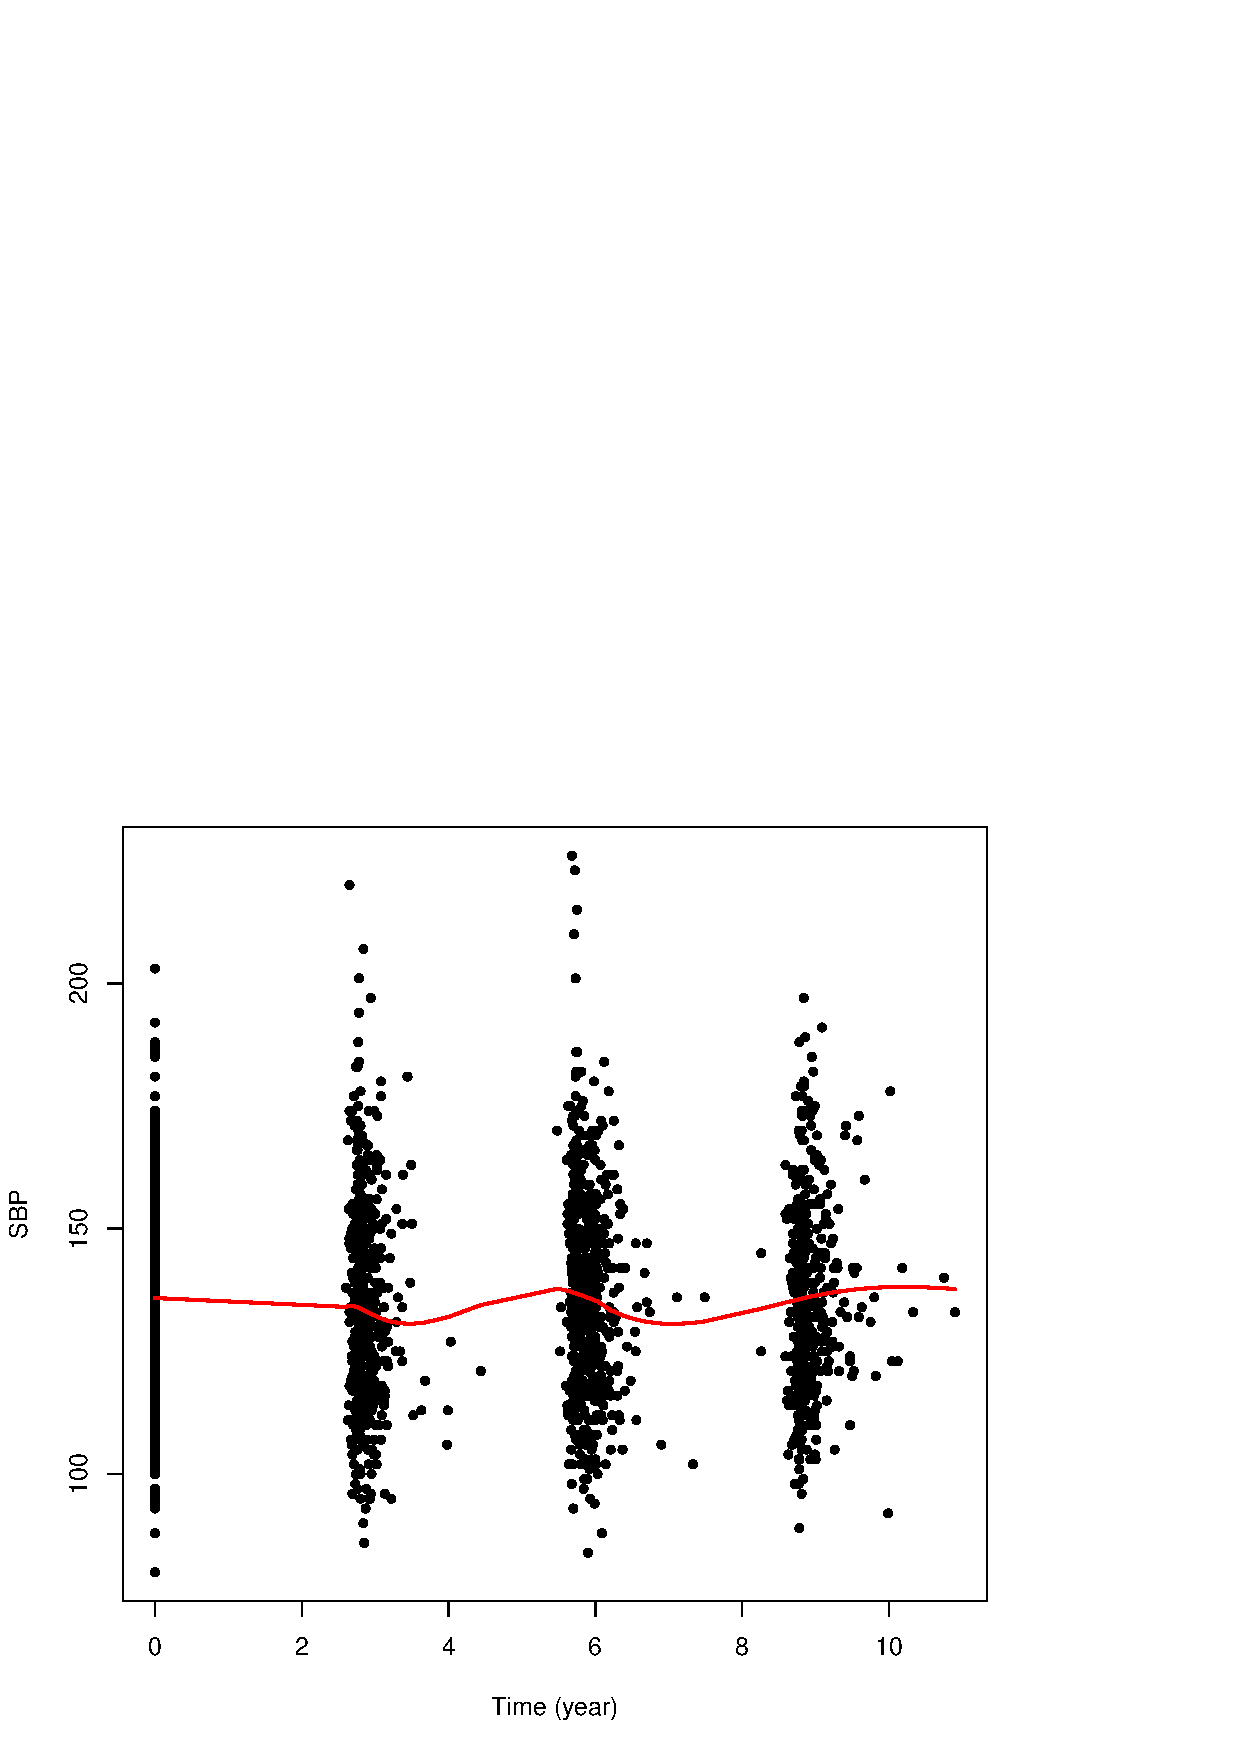
\includegraphics[width=\columnwidth]{SBP_loess.pdf}
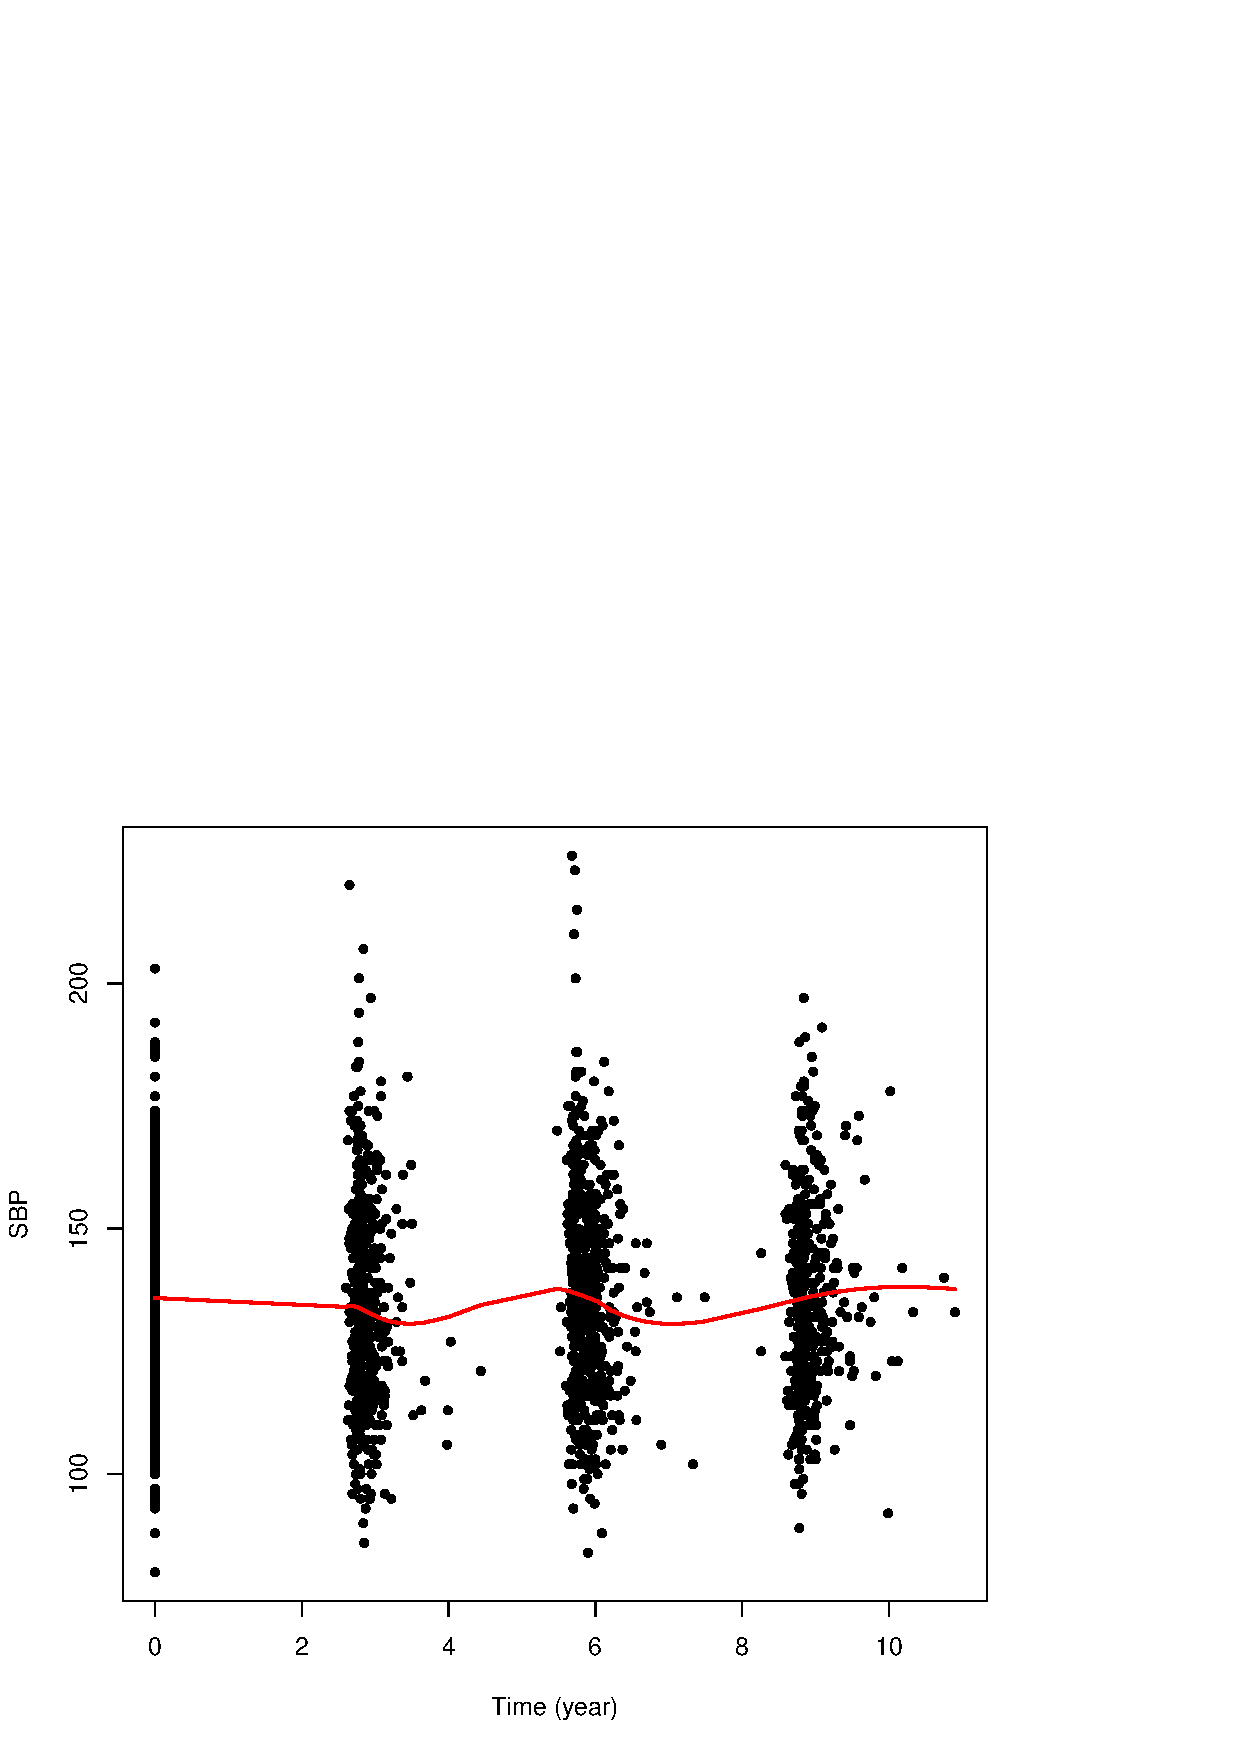
\includegraphics[scale=0.6]{SBP_loess.pdf}
\caption{Scatter plot with LOESS curve of longitudinal SBP measures in the study cohort.}
\label{fig:p2_sbp_loess}
\end{figure}

In data analysis, follow-up time is converted from days to years and the first examination date is set to time 0; baseline age is centered by subtracting the overall mean, and total-cholesterol is standardized to have mean 0 and standard deviation 1. We consider the following QRJM:
\small{
\begin{equation*}\label{eqn:p2data_joint}
\left\{
\begin{array}{l}
sbp_{i}(t) = m_{i}(t) + \varepsilon_{i}(t) = \beta_0 + \beta_1 age_{0i} + \beta_2 chol_i + \beta_3 I_{hyper-med_i}+ \beta_4 t + {u}_{i1} + u_{i2} t + \varepsilon_{i}(t)\\
r_i(t|\mathcal{M}_{it};  \boldsymbol{\gamma}, \alpha) = \sum_{k=1}^3v_i\lambda_kI_k(t)\exp(\gamma_1 I_{male_i} + \gamma_3 I_{smoke_i} + \gamma_4I_{diabetes_i} + \alpha m_i(t))
\end{array}
\right.
\end{equation*}
}
where we assume  $\varepsilon_{i}(t)\sim ALD(0, \sigma, \tau)$. $age_0$ is the baseline age at the first examination, $chol$ stands for the total-cholesterol level (mg/dL), $I_{hyper-med}$ is the variable indicating whether an individual had taken hypertension lowering medication, $t$ is the follow-up time, and $u_{i1}$ and $u_{i2}$ are subject-specific random intercept and slope to account for the within subject correlation and between subject variation. In the recurrent event submodel, we specify a piecewise constant baseline intensity function with three time intervals, where $\lambda_k$ is the hazard rate for time interval $[t_{k-1}, t_{k})$, that is $I_k(t)=1$ if $t\in[t_{k-1}, t_{k})$ and 0 otherwise. Knots $t_1$ and $t_2$, used to define piecewise constant time intervals, are selected as the 33.3\% and 66.7\% percentiles of the ordered follow-up time; while $t_0$ = 0 and $t_3$ is the maximum of follow-up time. We also include a frailty term $v_i$ in the recurrent event model that introduces correlation of multiple CHD events within the same individual. Other model covariates include indicator variables for male ($I_{male}$), ever smoke ($I_{smoke}$), and diabetes mellitus ($I_{diabetes}$). In the QRJM, the true underlying longitudinal measure of SBP is treated as a time dependent covariate in the recurrent event process and $\alpha$ is the association parameter governing the dependence between these two processes. Two chains with diverse initial values are initiated in the Bayesian inference algorithm and the chains are considered to converge if the potential scale reduction factors (PSRF) for all parameters are below 1.1.


\subsubsection{Inference Results for ARIC data}\label{sec:p2data_results}
Inference results from five different quantiles (0.05, 0.25, 0.50, 0.75, and 0.95) of SBP are shown in Table~\ref{p2realdata_inference} as well as visualized in Figure~\ref{p2_jm_infer}. In the longitudinal SBP process, older participants generally have higher SBP level and the effect of baseline age is consistently positive across all five selected quantiles of SBP. For example, one year increase in baseline age is associated with 0.037 (95\% CI: (0.028, 0.047)) unit increase in the median (i.e., $\tau=0.50$) of standardized SBP in the study cohort when controlling for other covariates. Total cholesterol level is negatively associated with SBP; however, the effects are not significant across all five quantiles. In general, people who took hypertension medications have significantly lower SBP and the effect of taking hypertension medications is larger at higher levels of SBP. Moreover, it is interesting to see that follow-up time has a significantly positive effect on higher quantiles of SBP (i.e., $\tau=0.75$ and 0.95) while for lower quantiles ($\tau=0.05$, 0.25, and 0.50) the effect is not significant. This finding can be an important indication that among the hypertension patients who originally have excessively higher SBP deteriorate even faster than those with lower SBP.

In the recurrent CHD event process, we see all positive association between the five conditional quantiles of SBP and the risk of CHD event, which coincide with our expectation as well as previous findings from ARIC data. However, the degree of association between these two processes varies among the conditional quantiles and is found to be strongest at the conditional median of SBP (relative risk:1.25, 95\% CI: (1.02, 1.53)) among the five selected quantiles. For other regression covariates, diabetic patients are at significantly higher risk of having recurrent CHD event compared with non-diabetic. For example, when controlling for other factors, the risk of having additional CHD event is 2.3 times higher ($\exp(0.85)$, 95\% CI: (1.46, 3.85)) for people with diabetes than those who are free of the disease at $\tau=0.5$. We also observed the posterior effect of diabetes decreases as quantile increases. This indicates that the effect of diabetes on the risk of recurrent CHD event is less important for patients with higher SPB. Although  male patients and ever smokers are also at higher risk of experiencing CHD events, the relative risks are statistically insignificant compared with female and never smokers respectively.

\newpage
\thispagestyle{lscape}
\pagestyle{lscape}
\begin{landscape}
\doublespacing
% \begin{sidewaystable}[H]
\begin{table}[H]
\centering
\caption{ARIC data analysis: Parameter estimation and 95\% credible interval (in parenthesis) from QRJM at five quantiles.}
\label{p2realdata_inference}
\resizebox{\linewidth}{!}{
\begin{tabular}{lccccc}
  \hline
  & $\tau=0.05$ & $\tau=0.25$ & $\tau=0.50$ & $\tau=0.75$ & $\tau=0.95$\\
\hline
\multicolumn{6}{c}{\textit{longitudinal SBP process}}  \\
  intercept & -0.374 (-0.478, -0.274) & -0.023 (-0.118, 0.074) & 0.447 (0.352, 0.554) & 0.872 (0.775, 0.978) &1.187 (1.079, 1.300)\\
  age$_0$ & 0.035 (0.026, 0.044) & 0.034 (0.025, 0.044) & 0.037 (0.028, 0.047) & 0.040 (0.030, 0.050) & 0.043 (0.031, 0.052)\\
  total-chol.(mg/dL) & -0.020 (-0.073, 0.033) & -0.026 (-0.081, 0.032) & -0.022 (-0.078, 0.037) & -0.013 (-0.073, 0.047) & -0.022 (-0.076, 0.032)\\
  hypertension medicine & -0.583 (-0.710, -0.467) & -0.652 (-0.773, -0.538) & -0.725 (-0.842, -0.609) & -0.730 (-0.868, -0.593) & -0.787 (-0.924, -0.660)\\
  follow-up time (yr) & 0.008 (-0.003, 0.018) & 0.006 (-0.006, 0.019) & 0.011 (-0.001, 0.022) & 0.016 (0.004, 0.029) & 0.019 (0.005, 0.033)\\
  \multicolumn{6}{c}{\textit{recurrent CHD event process}}  \\
  association & 0.163 (-0.003, 0.332) & 0.207 (0.011, 0.405) & 0.226 (0.019, 0.428) &  0.205 (0.034, 0.374) &0.162 (0.028, 0.288)\\
  male & 0.191 (-0.152, 0.548) & 0.185 (-0.170, 0.528) &  0.160 (-0.187, 0.507) & 0.132 (-0.205, 0.477) & 0.110 (-0.234, 0.458)\\
  ever  smoke & 0.291 (-0.044, 0.641) & 0.271 (-0.070, 0.613) & 0.216 (-0.121, 0.552) & 0.165 (-0.177, 0.493) & 0.163 (-0.184, 0.485)\\
  diabetes & 0.918 (0.424, 1.399) & 0.895 (0.409, 1.376) & 0.850 (0.381, 1.349) & 0.811 (0.352, 1.318) & 0.818 (0.333, 1.301)\\
  $\lambda_1$ & 0.011 (0.010, 0.013) & 0.011 (0.010, 0.013) & 0.011 (0.010, 0.012) & 0.011 (0.010, 0.012) & 0.011 (0.010, 0.012)\\
  $\lambda_2$ & 0.028 (0.020, 0.036) & 0.027 (0.019, 0.035) & 0.026 (0.018, 0.034) & 0.024 (0.017, 0.032) & 0.024 (0.017, 0.032)\\
  $\lambda_3$ & 0.073 (0.037, 0.113) & 0.072 (0.036, 0.111) & 0.067 (0.034, 0.105) & 0.065 (0.033, 0.103) & 0.066 (0.034, 0.103)\\
   \hline
\end{tabular}
}
\end{table}
% \end{sidewaystable}
\end{landscape}

\restoregeometry
\pagestyle{plain}

\newpage
\begin{figure}[H]
\centering
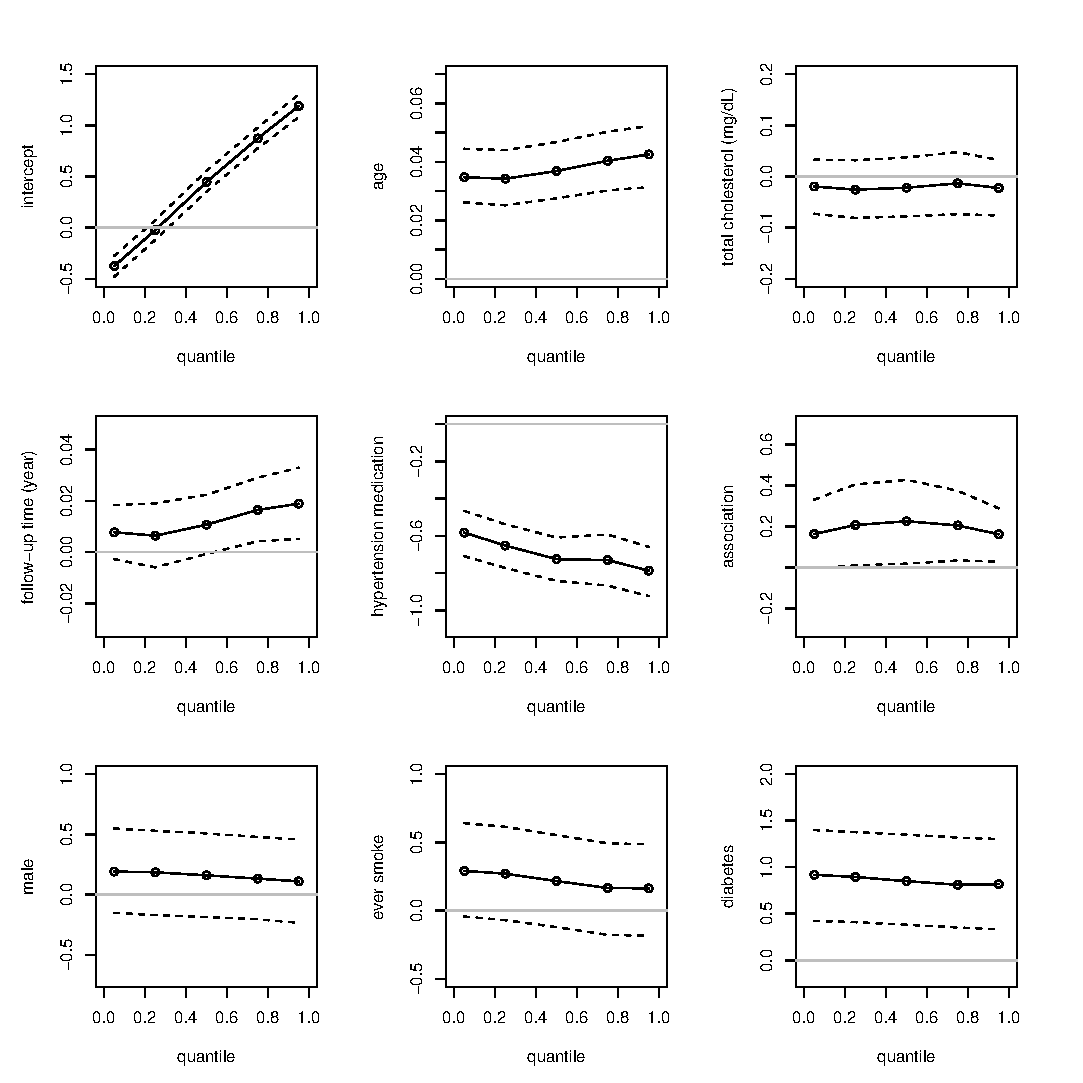
\includegraphics[width=\textwidth]{0.plots/p2_JM_inference_covs.eps}
\caption{ARIC data analysis: Posterior mean (solid line) and point-wise 95\% credible interval (dashed lines) of parameter estimation against different quantiles.}
\label{p2_jm_infer}
\end{figure}




% \end{document}

% \documentclass{article}
% \usepackage[utf8]{inputenc}
% \usepackage{fullpage}
% \usepackage {setspace}
% \usepackage[hang,flushmargin]{footmisc} %control footnote indent
% \usepackage{url} % for website links
% \usepackage{amssymb,amsmath}%for matrix
% \usepackage{graphicx}%for figure
% \usepackage{appendix}%for appendix
% \usepackage{float}
% \usepackage{multirow}
% \usepackage{longtable}
% \usepackage{morefloats}%in case there are too many float tables and figures
% \usepackage{caption}
% \usepackage{subcaption}
% \usepackage{listings}
% \captionsetup[subtable]{font=normal}
% \usepackage{color}
% \usepackage{hyperref}
% \usepackage[round]{natbib}
% \usepackage{appendix}
% \usepackage{listings}
% \usepackage{courier}
% \usepackage{color}


% \lstset{style=mystyle}


% \setlength{\parindent}{0em}
% \setlength{\parskip}{0.5em}


% \graphicspath{{0.plots/}}



% \begin{document}



\subsection{Discussion}\label{sec:p2discussion}
% What is done in this work, including data analysis part.
In the application of conventional JM methodologies for longitudinal and recurrent event data, we usually encountered two limitations: first, the normality assumption of the random error in the LMM was not realistic, and no obvious transformation of the longitudinal outcome to produce residual normality was applicable. This limitation is confirmed by our simulation study where LMJM tends to provide biased point estimates as well as lower coverage probabilities for model parameters when the longitudinal data are non-normal. Second, LMJM models only the conditional mean of the outcome; however, in our (and other) clinical research applications, it is more desirable to consider the tails of the biomarker distribution. For example, in our application of the ARIC data, higher level of SBP imposes higher risk of recurrent CHD event and the association between the two outcomes varies according to different conditional quantiles.

Our work on QRJM that uses an LQMM for the longitudinal process provides an alternative and more flexible way for modeling the joint distribution of longitudinal and recurrent event outcomes. The quantile-based estimators are more robust against skewness in the data, and as a result, our approach provides the flexibility to use median or quantile regression instead of mean regression when outliers are concerned. Moreover, QRJM provides a set of estimates at different quantiles of the longitudinal outcome variable, which can have practical meaning when the lower or higher quantile of the outcome is more relevant to health-related questions. In general, we show via simulation and application that QRJM not only inherits the good properties of a LMJM, but adds flexibility to the modeling procedure.

In this work, we developed a Gibbs sampler algorithm to fit the proposed model, where the likelihood function of the longitudinal quantile regression is written under the location-scale representation of the ALD distribution. The proposed algorithm is straightforward to implement in existing Bayesian software. The current version of Gibbs sampler, which is implemented in \textsf{JAGS} software, uses a piecewise constant baseline hazard function in the recurrent event submodel. However, other functional forms can also be considered and the integration of the hazard function can be approximated using Simpson's rule. In the real data application, we illustrate the flexibility of QRJM and its advantages over the LMJM by jointly modeling the risk of developing recurrent CHD event and repeated SBP measurements. QRJM is able to provide us with more informative insights into the disease progression and the association between the two disease processes in terms of various quantile-based estimations.

Our novel extension of JM in using LQMM for the longitudinal outcome finds practical importance in many clinical applications. Studying covariate effects on the conditional mean of the outcome gives us an idea about how treatment and other factors may affect disease progression in the population on average; however, it is limited to be too general and those effects could be dramatically different depending different quantiles of the outcome under investigation. Particularity, higher or lower tail of the longitudinal biomarker is often associated with worse medical condition in patients and leads to higher risk of disease. If treatment effect on tails of the outcome is significantly different from the average effect, treating different groups of patients using the exact same way won't be as effective as we tailor the treatment strategy according to patient-specific situation.

% Method summary and software.
% Limitation and
% Further work.

Currently, in the proposed QRJM we only consider an LQMM and a PHM for the longitudinal and recurrent event outcomes respectively. However, other modeling strategies can also be considered to extend the proposed method. For example, for the longitudinal outcome, nonlinear QR \citep{koenker1996interior} or even nonparametric QR \citep{le2005nonparametric} models can be used in stead of linear QR. In the recurrent event submodel, accelerated failure time model can be consider as another parametric formulation for event times and counting process approach is another nonparametric option.

% A question arises naturally from using quantile regression is which quantile should we choose? The answer is not unique and should depend on the specific research aim.

%All is done in \LaTeX \cite{knuth1986texbook}.
%
%
% \bibliographystyle{plainnat}%%%%%%%%%%%%%%%%%%%%
% \addcontentsline{toc}{section}{References}
% \bibliography{QRJM}


% \end{document}

\newpage
% \documentclass[12pt]{article}
% \usepackage[text={7.1 in, 8 in}, top=1.75in, left=0.69in]{geometry}
% \usepackage[round]{natbib}
% \usepackage[utf8]{inputenc}
% \usepackage{fullpage}
% \usepackage {setspace}
% \usepackage[hang,flushmargin]{footmisc} %control footnote indent
% \usepackage{url} % for website links
% \usepackage{amssymb,amsmath}%for matrix
% \usepackage{graphicx}%for figure
% \usepackage{appendix}%for appendix
% \usepackage{float}
% \floatstyle{plaintop}
% \restylefloat{table}
% \usepackage{multirow}
% \usepackage{longtable}
% \usepackage{morefloats}%in case there are too many float tables and figures
% \usepackage{caption}
% % \usepackage{subcaption}
% \usepackage{subfig}
% \captionsetup[subtable]{font=normal}
% \usepackage{hyperref}
% \usepackage{courier}
% \usepackage{color}
% \usepackage{setspace}
% \usepackage{rotating} % rotate table by some degree
% \usepackage{rotfloat}
% \usepackage{mwe}
% \usepackage{listings}
% \usepackage{titling}
% \usepackage{lipsum}
% \usepackage[export]{adjustbox}




% \graphicspath{{figures/}}

% \begin{document}
% \author{\small{\bf Ming Yang, Sheng Luo,
% and Stacia M. DeSantis}\\
% \small{Department of Biostatistics, The University of Texas Health Science Center at Houston}}
% \date{}
% \title{\large{\bf Web-based Supplementary Material for ``Model Estimation and Dynamic Prediction in Joint Modeling Using Longitudinal Quantile Regression''}}
% \maketitle{}


\subsection*{Appendices}
\addcontentsline{toc}{subsection}{Appendices}
\renewcommand{\thesubsubsection}{\Alph{subsubsection}}


\subsubsection{Additional simulation results}\label{sec:p2appendix_simulation}
In Scenario 2, data are generated from Laplace distribution (i.e., ALD with $\tau=0.5$). LMJM methods still produce noticeably larger bias and lower CP compared to the true model.

\begin{table}[H]
\centering
\caption{Simulation study: Inference results for data generated from ALD with $\tau$ = 0.50 (Scenario 2).}
\label{tab:p2simsce2}
\begin{tabular}{clccccccc}
\hline
& & \multicolumn{3}{c}{QRJM ($\tau=0.5$, true model)} & & \multicolumn{3}{c}{LRJM}\\
\hline
 & & bias & MSE & CP && bias & MSE & CP \\
 \cline{3-5}  \cline{7-9}
  \multirow{7}{*}{n=250} & $\beta_1$ & 0.005 & 0.007 & 0.97 && 0.006 & 0.008 & 0.97 \\
  & $\beta_2$ & -0.027 & 0.017 & 0.94 && -0.027 & 0.019 & 0.93 \\
  & $\beta_3$ & 0.022 & 0.004 & 0.94 && 0.026 & 0.005 & 0.94 \\
  & $\sigma$ & -0.002 & 0.001 & 0.94 &&  - & - & - \\
  & $\alpha$ & 0.016 & 0.004 & 0.94 && 0.003 & 0.006 & 0.95 \\
  & $\gamma$ & 0.006 & 0.005 & 0.96 && 0.005 & 0.006 & 0.93 \\
  & $r_0$ & 0.011 & 0.013 & 0.95 && 0.011 & 0.014 & 0.95 \\
   \hline
 \multirow{7}{*}{n=500} & $\beta_1$ & -0.001 & 0.004 & 0.93 && -0.001 & 0.005 & 0.93 \\
  & $\beta_2$ & -0.006 & 0.007 & 0.96 && -0.006 & 0.008 & 0.96 \\
  & $\beta_3$ & 0.014 & 0.002 & 0.95 && 0.016 & 0.002 & 0.95 \\
  & $\sigma$ & 0.002 & 0.001 & 0.94 &&  - & - & - \\
  & $\alpha$ & 0.003 & 0.002 & 0.92 && 0.017 & 0.003 & 0.95 \\
  & $\gamma$ & 0.008 & 0.003 & 0.93 && 0.008 & 0.004 & 0.92 \\
  & $r_0$ & -0.019 & 0.008 & 0.93 && -0.022 & 0.008 & 0.95 \\
   \hline
\end{tabular}
\end{table}



In Scenario 3, data are simulated from QRJM with $\tau=0.75$. Results are similar to what we observed when $\tau=0.25$ in Scenario One.

\begin{table}[H]
\centering
\caption{Simulation study: Inference results for data generated from ALD with $\tau$ = 0.75 (Scenario 3).}
\label{tab:p2simsce3}
\adjustbox{max width=\textwidth}{
\begin{tabular}{clccccccccccc}
\hline
& & \multicolumn{3}{c}{QRJM ($\tau=0.75$, true model)} & & \multicolumn{3}{c}{QRJM ($\tau=0.5$)} & & \multicolumn{3}{c}{LRJM}\\
\hline
 & & bias & MSE & CP && bias & MSE & CP & & bias & MSE & CP\\
 \cline{3-5}  \cline{7-9} \cline{11-13}
   \multirow{7}{*}{n=250} & $\beta_1$ & 0.004 & 0.007 & 0.96 && 0.003 & 0.017 & 0.91 && 0.173 & 0.053 & 0.79\\
  &   $\beta_2$ & -0.026 & 0.018 & 0.93 && -1.119 & 1.282 & 0.00 && -1.813 & 3.343 & 0.00\\
  &   $\beta_3$ & 0.025 & 0.004 & 0.93 && -0.119 & 0.022 & 0.65 && 0.001 & 0.012 & 0.92\\
  &   $\sigma$ & -0.003 & 0.001 & 0.93 && -0.333 & 0.111 & 0.00 && - & - & - \\
  &   $\alpha$ & 0.016 & 0.004 & 0.96 && -0.037 & 0.014 & 0.84 && -0.227 & 0.058 & 0.25\\
  &   $\gamma$ & 0.009 & 0.005 & 0.95 && -0.047 & 0.008 & 0.93 && -0.068 & 0.012 & 0.87\\
  &   $r_0$ & 0.010 & 0.013 & 0.96 && 2.155 & 4.781 & 0.00 && 4.469 & 20.237 & 0.00\\
   \hline
  \multirow{7}{*}{n=500} & $\beta_1$ & -0.006 & 0.004 & 0.93 && -0.008 & 0.009 & 0.92 && 0.149 & 0.044 & 0.67\\
  & $\beta_2$ & -0.014 & 0.009 & 0.93 && -1.080 & 1.181 & 0.00 && -1.777 & 3.187 & 0.00\\
  & $\beta_3$ & 0.024 & 0.002 & 0.90 && -0.126 & 0.019 & 0.41 && -0.022 & 0.011 & 0.93\\
  & $\sigma$ & 0.003 & 0.001 & 0.96 && -0.327 & 0.108 & 0.00 && - & - & - \\
  & $\alpha$ & 0.001 & 0.003 & 0.94 && -0.023 & 0.006 & 0.87 && -0.153 & 0.430 & 0.08\\
  & $\gamma$ & 0.004 & 0.003 & 0.94 && -0.041 & 0.005 & 0.87 && -0.069 & 0.010 & 0.77\\
  & $r_0$ & -0.011 & 0.008 & 0.96 && 2.053 & 4.301 & 0.00 && 4.359 & 19.350 & 0.01\\
   \hline
\end{tabular}
}
\end{table}






\newpage
\thispagestyle{lscape}
\pagestyle{lscape}
\begin{landscape}
\doublespacing
% \begin{sidewaystable}[H]
\subsubsection{Summary table of study cohort characteristics}
\begin{table}[H]
\centering
\caption{Baseline characteristics of study cohort with stratification by SBP level}
\label{tab:p2cht_baseline}
% \adjustbox{max width=\textwidth}{
\resizebox{\linewidth}{!}{
\begin{tabular}{llcccc}
\hline
& & \multicolumn{3}{c}{SBP groups (mm Hg)} \\
\cline{3-5}
 Characteristics\textsuperscript{$\dagger$} & Total (657) & $<$ 120 (133, 20.2\%)  & [120, 140) (217, 33.0\%)& $\ge$ 140 (307, 46.7\%) & $p$-value\textsuperscript{*}\\
 \hline
 Age & 56.4 (5.8) & 55.0 (5.7) & 55.7 (6.0) & 57.4 (5.4) & $<$0.001\\
 SBP & 135.9 (18.5) & 110.5 (6.9) & 129.2 (5.7) & 151.6 (11.2) & $<$0.001\\
 Cholesterol (mg/dL)& 215.9 (41.7) & 215.1 (42.1) & 214.0 (42.0) & 217.6 (41.7) & 0.60 \\
 Gender (male) & 341 (51.9) & 64 (48.1) & 117 (53.9) & 160 (52.1) & 0.57\\
 Ever smoke (yes) & 379 (57.5) & 81 (60.9) & 126 (58.1) & 172 (56.0) & 0.63\\
 Hypertension medication (yes) & 445 (67.7) & 132 (99.2) & 196 (90.3) & 117 (38.1) & $<$0.001\\
 Diabetes (yes) & 90 (13.7) & 15 (11.3) & 27 (12.4) & 48 (15.6) & 0.38\\
   \hline
   \multicolumn{6}{l}{\textsuperscript{$\dagger$}\footnotesize{mean (sd) for continuous variables and frequency (percentage) for categorical variables.}}\\
   \multicolumn{6}{l}{\textsuperscript{*}\footnotesize{Comparing three SBP groups; ANOVA test for continuous variables and $\chi^2$ test for categorical variables.}}\\
\end{tabular}
}
\end{table}
% \end{sidewaystable}
\end{landscape}

\restoregeometry
\pagestyle{plain}





\newpage
\subsubsection{\textsf{JAGS} model file}
\textsf{JAGS} model file to fit QRJM of longitudinal and recurrent event data.
{\small
\begin{verbatim}
model{
      k1 <- (1-2*qt)/(qt*(1-qt))
      k2 <- 2/(qt*(1-qt))

      # prior of random effects
      for (i in 1:I){ # I: unique subject id
        # prior for random effects
          u[i] ~ dnorm(0, tau)
      } # end of loop i

      # longitudinal process, BQR mixed model using ALD representation
      for (j in 1:N_l){ # N_l: number of longitudinal observations
          er[j] ~ dexp(sigma)
          mu[j] <- beta1*X1_l[j] + beta2[X2_l[j]] + beta3*t[j] + u[id_l[j]]
          			+ k1*er[j]
          prec[j] <- sigma/(k2*er[j])
          y[j] ~ dnorm(mu[j], prec[j])
      } #end of j loop

    # recurrent events part, baseline hazard is set to constant c
      for(k in 1:I){
        for (l in (s[k]+1):s[k+1]){
          m1[l] <- beta1*X1[k]+beta2[X2[k]]+beta3*Ri1[l]+u[id_r[l]]
          m2[l] <- beta1*X1[k]+beta2[X2[k]]+beta3*Ri2[l]+u[id_r[l]]
          res[l] <- (exp(gamma*W[k]+alpha*m2[l])
                       -exp(gamma*W[k]+alpha*m1[l]))/(alpha*beta3)
          S[l] <- exp(-c*res[l])
          risk[l] <- c*exp(gamma*W[k] + alpha*m2[l])
          L[l] <- pow(risk[l], event[l])*S[l]/1E+08
          zeros[l] ~ dpois(-log(L[l]))
        } # end of l loop
      }#end of k loop

    # priors for other parameters
      alpha ~ dnorm(0, 0.0001)
      beta1 ~ dnorm(0, 0.0001)
      beta2[1] <- 0
      beta2[2] ~ dnorm(0, 0.0001)
      beta3 ~ dnorm(0, 0.0001)
      gamma ~ dnorm(0, 0.0001)
      sigma ~ dgamma(0.001, 0.001)
      c ~ dunif(0.01, 10)
      tau <- pow(var, -2)
      var ~ dunif(0, 1000)
  }
\end{verbatim}
}

\addcontentsline{toc}{subsection}{References}
\putbib[paper2]
\end{bibunit}

%%%%%%%%%% Journal article three %%%%%%%%%%%%%%%%%%%%%%%%%%%%
\newpage
\section{Journal Article 3}

{\bf Title of Journal Article}\\
Bayesian Quantile Regression Joint Models: Dynamic Predictions of Recurrent Event Probability\\
{\bf Journal proposed for article submission: Statistics in Medicine} \\


\newpage
% \begin{center}
\title{Bayesian Quantile Regression Joint Models: Dynamic Predictions of Recurrent Event Probability}
% \end{center}

\author{}
\date{}

\maketitle


\begin{center}
{\bf Abstract}
\end{center}

Joint models (JM) of longitudinal and time-to-event outcomes have received increasing interest recently. A novel use of JM is to make dynamic predictions of event probability from observed longitudinal and time-to-event data. In contrast to the extensive literature on JM of longitudinal and single time-to-event (e.g. death) data, less attention has been received for the JM of longitudinal and recurrent event data. In this work, we develop a Gibbs sampling algorithm for making subject-specific dynamic predictions of the risk of event recurrence based the JM of longitudinal and recurrent event outcomes. In our JM, differently from traditional JM, we adopt a linear quantile mixed model (LQMM) instead of the frequently used linear mixed model (LMM) for the longitudinal outcome. Compared with LMM, as a quantile regression based model, LQMM is more robust against non-normality or outliers in the data. Moreover, LQMM is more flexible than LMM in that it allows investigation of covariate effects on any conditional quantile of the outcome. In the proposed Bayesian algorithm, predictions are calculated based on the entire longitudinal trajectory as well as the recurrent events history and can be dynamically updated when new data from either (or both) outcome is available. In addition, implemented through the MCMC technique, the uncertainty of the predictive inference is fully captured in the posterior distribution and no asymptotic theory is needed to derive the standard error. It is straightforward to code and implement the proposed Bayesian predictive algorithm in existing software. We assess the performance of our model through extensive simulation studies and apply it to dynamically predict the probability of recurrent coronary heart diseases for the Atherosclerosis Risk In Communities Study cohort.

% Recurrent event outcome (e.g. multiple heart failures, cancer recurrence, hospital readmissions, etc.)  is commonly encountered in longitudinal biomedical studies. In those studies, recurrent events can be an important outcome of interest in monitoring disease progression or health condition of the study participants in addition to some continuous longitudinal disease biomarkers. For example, in the Atherosclerosis Risk In Communities Study (ARIC), recurrent event outcomes, including coronary heart disease, stroke, and heart failure, etc., were collected from extensive cohort surveillance to monitor the health condition of the study cohort; meanwhile, repeated systolic blood pressure (SBP) were also measured at regular clinical visits. Previous studies using ARIC data found positive correlation between SBP and recurrent CHD events in the study cohort and patients who had CHD event(s) before were at higher risk to have disease recurrence in the future. This data mechanism motivates us to consider the joint models (JM) of longitudinal and recurrent event data for modeling the two outcomes together and furthermore to make predictions of future event probability based on historical data. In this paper, we propose to use the so-called linear quantile mixed model (LQMM) for the longitudinal outcome jointly with a proportional hazard model (PHM) for the recurrent event outcome under the JM framework. In contrast to the traditional JM methodology, where a linear mixed model (LMM) is commonly used for modeling the conditional mean of the longitudinal outcome, our quantile regression (QR) based model provides a more flexible, distribution-free way to study covariate effects at different quantiles of the longitudinal outcome. This becomes extremely important when higher (e.g. SBP) or lower (e.g. CD4 count) tail of the outcome is more relevant to clinical interest. Based on the proposed JM, we develop a novel dynamic prediction algorithm for predicting the probability of disease recurrence in the future. In this work, we develop a Gibbs sampling algorithm for the model inference as well as for dynamic predictions. The proposed Bayesian algorithm is based on the location-scale representation of the asymmetric Laplace distribution for LQMM and implemented through the MCMC technique. By using fully Bayesian algorithm the parameter uncertainly is conveniently incorporated into the predictions. We assess the performance of our Bayesian algorithms through extensive simulation studies and apply the proposed JM to dynamically predict the probability of recurrent CHD event for the ARIC cohort.



% Recurrent event data are commonly encountered in longitudinal follow-up studies related to biomedical science, econometrics, reliability, and demography. In many studies, recurrent events serve as important measurements for evaluating disease progression, health deterioration, or insurance risk. When analyzing recurrent event data, an independent censoring condition is typically required for the construction of statistical methods. In some situations, however, the terminating time for observing recurrent events could be correlated with the recurrent event process, thus violating the assumption of independent censoring. In this article, we consider joint modeling of a recurrent event process and a failure time in which a common subject-specific latent variable is used to model the association between the intensity of the recurrent event process and the hazard of the failure time. The proposed joint model is flexible in that no parametric assumptions on the distributions of censoring times and latent variables are made, and under the model, informative censoring is allowed for observing both the recurrent events and failure times. We propose a "borrow-strength estimation procedure" by first estimating the value of the latent variable from recurrent event data, then using the estimated value in the failure time model. Some interesting implications and trajectories of the proposed model are presented. Properties of the regression parameter estimates and the estimated baseline cumulative hazard functions are also studied.

{\bf Key words:} Bayesian; Dynamic predictions; Joint models; Linear quantile mixed model; Recurrent events.
\begin{bibunit}[apa]
% \documentclass{article}
% \usepackage[top=1.25in, bottom=1.1in, left=1.25in, right=1in]{geometry}
% \usepackage[utf8]{inputenc}
% \usepackage{fullpage}
% \usepackage {setspace}
% \usepackage[hang,flushmargin]{footmisc} %control footnote indent
% \usepackage{url} % for website links
% \usepackage{amssymb,amsmath}%for matrix
% \usepackage{graphicx}%for figure
% \usepackage{appendix}%for appendix
% \usepackage{float}
% \usepackage{multirow}
% \usepackage{longtable}
% \usepackage{morefloats}%in case there are too many float tables and figures
% \usepackage{caption}
% \usepackage{subcaption}
% \usepackage{listings}
% \captionsetup[subtable]{font=normal}
% \usepackage{color}
% \usepackage{hyperref}
% \usepackage[round]{natbib}

% %\usepackage{Sweave}
% \setlength{\parindent}{0em}
% \setlength{\parskip}{0.5em}


% \graphicspath{{0.plots/}}



% \begin{document}


\subsection{Introduction}

% JM in one or two sentences then talk about only the longitudinal part. Talk about the motivating data before introducing QR.

% Medical background of longitudinal and recurrent event data. Introduce the JM in analyzing these two types of data jointly.

% at least two longitudinal sequences of perhaps different data types are jointly recorded has received less attention so far, especially when one or more of the sequences consist of time-to-event data.

Joint analysis of longitudinal and time-to-event outcomes has been studied by many authors. However, majority of the literature focuses on JM of longitudinal and a single time-to-event (e.g. death) outcomes. For example, \cite{self1992modeling, tsiatis1995modeling, wulfsohn1997joint} developed the JM methods for survival analysis with a time dependent covariate measured with error. Despite the popularity of repeated time-to-event or recurrent event data, such as hospital readmissions, multiple cardiovascular diseases (e.g. stroke, heart failure, etc.), and cancer recurrences, etc., joint analysis of longitudinal and recurrent event outcomes has received less attention so far. To our knowledge, \cite{henderson2000joint} developed a shared random effects JM for longitudinal and recurrent event data. \cite{kim2012joint} considered a JM of longitudinal and recurrent event data with informative terminal event. And \cite{efendi2013joint} proposed a JM of longitudinal data and recurrent events that accommodates overdispersion. Moreover, disease recurrence is always one of the important clinical outcomes in longitudinal biomedical studies, which can be used to monitor disease progression and health condition of the patients. Predictions of future event probability based on historical data attracts increasing interest recently. Accurate predictions of disease probability can play an important role in disease intervention and prevention. The JM framework offers a novel way of making such personalized dynamic predictions of future event-free probability \citep{rizopoulos2011dynamic,taylor2013real}. However, so far, there is little work has been done on the dynamic predictions of event recurrences under the JM framework. 


In this paper, we propose a Gibbs sampling algorithm for making subject-specific predictions of the risk of event recurrence based on a new JM framework. Differently from conventional JM, we develop a quantile regression joint models (QRJM) framework that uses linear quantile mixed model (LQMM) in modeling the longitudinal continuous outcome; while the Cox proportional hazard model (PHM) is used for recurrent event outcome. There are several advantages of quantile regression (QR) based methods over the mean regression models (e.g. linear mixed model or LMM). First of all, LMM assumes normal error in the data; however, it is common that this normality assumption is violated in reality and no suitable transformation can be found. This is especially true when working with longitudinal data as the skewness changes over time. Moreover, LMM only models covariate effects on the conditional mean of the outcome; however, in many clinical settings it is more desirable to make inference at lower or higher quantiles of the outcome. For example, researchers used quantile regression QR to study risk factors of lower birth weight, in which they found several effects on the lower quantiles were significantly different from the mean effects \citep{koenker2001quantile}. This feature of QR find its great importance in biomedical studies, where individuals with extremer biomarker measurements are often at higher risk of disease or death. To our knowledge, \cite{farcomeni2015longitudinal} is the first one to incorporate an LQMM into a JM of longitudinal and terminal event data. However, there is little work has been do to use LQMM in the joint analysis with recurrent event data so far.


The development of the Gibbs sampler is based on the fact that minimizing the original QR loss function is equivalent to maximizing the likelihood function of the asymmetric Laplace distribution (ALD) \citep{yu2001bayesian}. It is relatively easy to make subject-specific predictions from the posterior samples of the fixed effects and the posterior predictive distributions of the random effects, which are direct results of our sampling algorithm. In addition, implemented through the MCMC technique, the uncertainty of the predictive inference is fully captured in the posterior distribution. We conduct extensive simulation studies to validate the proposed JM in model inference as well in making predictions. After that we apply the proposed algorithm to the Atherosclerosis Risk in Communities Study (ARIC) data \citep{aric1989atherosclerosis}, in which we investigate various covariate effects on different quantiles of the systolic blood pressure (SBP), its association with the recurrence of coronary heart disease (CHD), and make dynamic predictions of future recurrent CHD probability using historical SBP measures and recurrent CHD data. Moreover, such predictions can be dynamically updated whenever new data from either longitudinal or time-to-event outcome are available.

% Ignoring the dependence between the longitudinal and recurrent event processes and the fit models for these two outcomes separately will lead to loss of information and result in biased or inefficient inference results. 
% Traditional survival model with time-varying covariate may not be appropriate to use due to its limiting assumption of external time-dependent covariates that are not related to the event mechanism. This is especially true when we are interested in making predictions of the time-to-event outcome in the future, when the longitudinal biomarker is impossible to observe. Instead, joint models (JM) of longitudinal and time-to-event data overcome this limitation and can be used to model the association of the two processes simultaneously, based on which predictions of future event probability can also be made.

% By accommodating such joint processes, the simultaneous effects of covariates on the repeated instances of the same sequence, but also across sequences, can be modeled and examined. Also, subtle association processes, within a sequence as well as across sequences, can be made an integral part of the models.


%  WHY jm
% They overcome the time-dependent Cox model’s limiting assumptions of external time-varying covariates not related to the failure mechanism and diminish the linear mixed-effects models’ bias related to ignoring the association between longitudinal and time-to-event processes.

% 1. An internal time-dependent covariate is one where the change of the covariate over time is related to the behavior of the individual. For example, blood pressure, disease complications, etc.
% 2. An external or ancillary time-dependent covariate is one whose path is generated externally. For example, levels of air pollution.


% The key rule for time dependent covariates in a Cox model is simple and essentially the same as that for gambling: you cannot look into the future. A covariate may change in any way based on past data or outcomes, but it may not reach forward in time.


% literature review of JM: longitudinal and terminal, longitudinal and recurrent, recurrent and terminal or trivariate model.




% The development of the Gibbs sampler is based on the fact that minimizing the original QR loss function is equivalent to maximizing the likelihood function of the so-called asymmetric Laplace distribution (ALD) \citep{yu2001bayesian}. Moreover, the ALD can be further reparameterized using a location-scale mixture representation that leads to a combination of normal and exponential distributions \citep{kotz2001laplace, kozumi2011gibbs}.



% Accurate predictions of disease probability in the future can assist physicians to make specific treatment plan so that potential disease can be postponed or prevented in advance.  Our proposed Bayesian algorithm can be easily extended to make such dynamic predictions. A key feature of the dynamic predictions framework is that the predictive measures can be dynamically updated as additional longitudinal measurements and recurrent events information become available for the target subjects, providing instantaneous risk assessment.


% We applied the proposed model to the data derived from the Atherosclerosis Risk in Communities Study (ARIC). ARIC is a prospective epidemiologic study conducted to investigate the etiology of atherosclerosis and its clinical outcomes, and variation in cardiovascular risk factors, medical care, and disease by race, gender, location, and date.




%paper organization
The rest of this paper is organized as follows. In Section \ref{sec:p3methods}, we give details of the proposed statistical model and the Bayesian algorithms used for model inference and dynamic predictions. In Section \ref{sec:p3simulation}, we present simulation studies to validate the proposed methods. In Section \ref{sec:p3data}, we apply the proposed methods to the ARIC data to make dynamic predictions of CHD risk. We conclude the paper with a discussion in Section \ref{sec:p3discussion}.
% \bibliographystyle{plainnat}%%%%%%%%%%%%%%%%%%%%
% \addcontentsline{toc}{section}{References}
% \bibliography{QRJM}
% \end{document}




\subsection{Methods}\label{sec:p3methods}
% reformat the subsection section since it was changed in the appendix part of paper 1
\renewcommand{\thesubsubsection}{\thesubsection.\arabic{subsubsection}}
%%%%%%%%%%%%%%%%%%%%%%%%%%%

% Notice that Equation (\ref{eqn:p3lo_sc_lh}) actually takes the form of a normal distribution thus it is possible to implement the sampling algorithm directly in some Bayesian inference software like \textsf{BUGS}.
%%%%%%%%%%%%%%%%%%%%%%%%%%%
\subsubsection{Joint Models Using Longitudinal Quantile Regression}
% We then extend the linear model JM (LMJM), by replacing the LMM with an LQMM for the longitudinal process.
% Currently, for simplicity, we assume the death time is uninformative, i.e., independent of censoring time and the longitudinal process.
For subject $i$, let $T_{ik}^*$ be the underlying true $k$th recurrent event time and $C_i$ be the censoring time, which is assumed to be independent of both outcomes. Then $T_{ik} = $\mbox{ min}($C_i, T_{ik}^*)$, for $k=1, \cdots, K$, is the observed $k$th event time, where $K$ is the total number of recurrent events for subject $i$. Let $\Delta_{ik}$ be the recurrent event indicator at time $T_{ik}$ which is defined as $\Delta_{ik} = I(T_{ik}^* < C_i)$, and $I(\cdot)$ is the indicator function. A $k$th recurrent event is observed at time $T_{ik}$ if $\Delta_{ik}=1$, i.e. $T_{ik}^* < C_i$; other wise, $\Delta_{ik}=0$.

Let $Y_{i}(t)$ be the continuous longitudinal outcome for subject $i$ measured at time $t$. Note that we can only observe $Y_{i}(t)$ when $t\le C_i$, and the complete longitudinal trajectory up to follow-up time $t$ for subject $i$ can be written as $\mathcal{Y}_{i}(t)=\{Y_{i}(s): 0\le s\le t\}$. We denote the true underlying longitudinal measurement with $m_{i}(t)$ and his/her complete history of true longitudinal process as $\mathcal{M}_{i}(t)=\{m_{i}(s): 0\le s \le t\}$. We propose a new JM that uses longitudinal quantile mixed model (LQMM) as follows:
\begin{equation}\label{eqn:p3joint}
\left\{
\begin{array}{l}
Y_{i}(t) = m_{i}(t) + \varepsilon_{i}(t) = {\boldsymbol X}_{i}^{\top}(t)\boldsymbol{\beta}_{\tau} + {\boldsymbol Z}_{i}^{\top}(t){\boldsymbol u}_i + \varepsilon_{i}(t), \varepsilon_{i}(t)\sim ALD(0, \sigma, \tau)\\
r_i(t|\mathcal{M}_{i}(t), {\boldsymbol W}_i;  \boldsymbol{\gamma}_{\tau}, \alpha_{\tau}) = r_{i0}(t)\exp({\boldsymbol W}_i^{\top}\boldsymbol{\gamma}_{\tau} + \alpha_{\tau}({\boldsymbol X}^{\top}_{i}(t)\boldsymbol{\beta}_{\tau} + {\boldsymbol Z}^{\top}_{i}(t){\boldsymbol u}_{i}))
\end{array}
\right.
\end{equation}

\noindent where in the LQMM for the longitudinal process, $\boldsymbol{X}_{i}(t)$ are $p-$dimensional fixed effect covariates and $\boldsymbol{Z}_{i}(t)$ are $k-$dimensional multivariate normal covariates associated with the $k-$dimensional random effects $\boldsymbol{u}_i$. The submodel for recurrent event process takes the format of Cox proportional hazards model (PHM) where $r_{i0}(\cdot)$ is the baseline intensity function and $\boldsymbol{W}_{i}$ are $q-$dimensional fixed effect covariates that are only associated with event time (not the longitudinal outcome). In Equation (\ref{eqn:p3joint}), individual heterogeneity is captured by ${\boldsymbol Z}_{i}^{\top}(t){\boldsymbol u}_i$, which is the deviation of subject $i$ from the population average. Meanwhile, these two models are linked by treating the longitudinal outcome as a time dependent covariate in the recurrent event process, and the degree of associations is measured by parameter $\alpha$.

In quantile regression, all parameter estimators are functions of the quantile. This is also true in the proposed JM. That is, parameter estimations in the recurrent events submodel, such as $\alpha$ and $\boldsymbol{\gamma}$, also change depending which $\tau$ is chosen. Quantile regression provides us the flexibility to conduct a study over the entire conditional distribution of the longitudinal outcome through fitting the model using a set of selected quantiles. Less varying values in the estimation indicates a relatively stable covariate effect on the outcome, and vice versa. If the interest lies only in assessing the effect on the lower or higher quantile of the longitudinal outcome and its association with the event process we may just fix the quantile and conduct the analysis.


\subsubsection{Bayesian Linear Quantile Mixed Model}\label{sec:p3BLQMM}
Consider the linear mixed effects model:
\begin{equation}\label{eqn:p3lmm}
Y_{i}(t) ={\boldsymbol X}_{i}^{\top}(t) \boldsymbol{\beta}+ {\boldsymbol Z}_{i}^{\top}(t)\boldsymbol{u}_i + \varepsilon_{i}(t),
\end{equation}

\noindent where $\boldsymbol{\beta}$ is a $p-$dimensional vector of fixed effects,  ${\boldsymbol X}_{i}(t)$ contains the corresponding fixed covariates, $\boldsymbol{u}_i$ is a $k-$dimensional vector of random effects for subject $i$, and ${\boldsymbol Z}_{i}(t)$ are the corresponding random covariates.

An LQMM assumes that the conditional quantile of the outcome is a linear function of the covariates, i.e.,
\begin{equation}\label{eqn:p3lqmm}
Q_{Y_{i}(t)|{\boldsymbol X}_{i}(t),{\boldsymbol Z}_{i}(t)}(\tau)={\boldsymbol X}_{i}^{\top}(t) \boldsymbol{\beta}+ {\boldsymbol Z}_{i}^{\top}(t)\boldsymbol{u}_i,
\end{equation}

\noindent where the $\tau$th quantile of a random variable $Y$ is defined as $Q_{Y}(\tau)=F_{Y}^{-1}(\tau)=\inf\left\{ y:F_{Y}(y)\geq\tau\right\}$, for $\tau\in [0, 1]$. Parameter estimations can then be obtained by minimizing the following loss function,

\begin{equation*}\label{eqn:p3loss_fun}
\hat{\boldsymbol{\beta}}_{\tau}=\underset{\boldsymbol{\beta}\in \mathbb{R}^{p}}{\mbox{arg min}}\sum_{i, t}\left[\rho_{\tau}\left(Y_{i}(t)-{\boldsymbol X}_{i}^{\top}(t)\boldsymbol{\beta} - {\boldsymbol Z}_{i}^{\top}(t)\boldsymbol{u}_i\right)\right],
\end{equation*}

\noindent where $\rho_{\tau}(\cdot)$ is defined as $\rho_{\tau}(Y)=Y(\tau-{I}{(Y<0)}).$


Above minimization problem can also be rephrased as a maximum-likelihood problem by assuming the random error $\varepsilon_{i}(t)$ in (\ref{eqn:p3lmm}) follows the asymmetric Laplace distribution (ALD) with location parameter equals 0, scale parameter $\sigma$ and skewness parameter $\tau$ \citep{koenker1999goodness,yu2001bayesian}:
\begin{equation*}
Y_{i}(t) ={\boldsymbol X}_{i}^{\top}(t) \boldsymbol{\beta}+ {\boldsymbol Z}_{i}^{\top}(t)\boldsymbol{u}_i + \varepsilon_{i}(t), \varepsilon_{i}(t)\sim ALD(0, \sigma, \tau).
\end{equation*}

This becomes clear when writing out the conditional likelihood function of the outcome variable:
\begin{equation*}\label{eqn:p3ald_lqmm}
\ell(Y_{i}(t)|\boldsymbol{\beta}_{\tau},\boldsymbol{u}_i,\sigma)=\frac{\tau(1-\tau)}{\sigma}\exp\left[-\rho_{\tau}\left(\frac{Y_{i}(t)-{\boldsymbol X}_{i}^{\top}(t)\boldsymbol{\beta}_{\tau}-{\boldsymbol Z}_{i}^{\top}(t)\boldsymbol{u}_i}{\sigma}\right)\right].
\end{equation*}

In Bayesian quantile regression context a Gibbs sampling algorithm for model inference is developed when we utilize a location-scale mixture representation of the ALD \citep{kotz2001laplace}. Under such parameterization the random error is represented as $\varepsilon_{i}(t)=\kappa_1e_{i}(t)+\kappa_2\sqrt{\sigma e_{i}(t)}v_{i}(t)$ with $v_{i}(t)\sim N(0,1), e_{i}(t)\sim\exp(1/\sigma)$ and
\[\kappa_1=\frac{1-2\tau}{\tau(1-\tau)}\hspace{2em} \kappa_2^2=\frac{2}{\tau(1-\tau)}.\]


This re-parameterization leads to the following linear mixed model,
\begin{equation*}\label{eqn:p3reformald2}
Y_{i}(t)={\boldsymbol X}_{i}^{\top}(t)\boldsymbol{\beta}_{\tau}+{\boldsymbol Z}_{i}^{\top}(t)\boldsymbol{u}_i+\kappa_1e_{i}(t)+\kappa_2\sqrt{\sigma e_{i}(t)}v_{i}(t),
\end{equation*}
\noindent or equivalently,
{\small
\begin{equation}\label{eqn:p3lo_sc_lh}
\ell(Y_{i}(t)|\boldsymbol{\beta}_{\tau},\boldsymbol{u}_i,e_{i}(t),\sigma)=\frac{1}{\sqrt{2\pi\kappa_2^2\sigma e_{i}(t)}}\exp\left[-\frac{(Y_{i}(t)-{\boldsymbol X}_{i}^{\top}(t)\boldsymbol{\beta}_{\tau}-{\boldsymbol Z}_{i}^{\top}(t)\boldsymbol{u}_i-\kappa_1e_{i}(t))^2}{2\kappa_2^2\sigma e_{i}(t)}\right].
\end{equation}
}


As discussed in \cite{yu2001bayesian}, irrespective of the actual distribution of the data, Bayesian quantile regression using ALD distribution works quite well for different error distributions and the performance is quite robust and satisfactory.




\subsubsection{The Recurrent Events Submodel}\label{sec:p3surv_submodel}
Assume a total number of $K$ events are observed for subject $i$ within the censoring time $C_i$, the likelihood function for recurrent event data can be written as:
\begin{eqnarray}\label{eqn:p3lik_sur}
\ell({\boldsymbol T}_i, \boldsymbol{\Delta}_i;\boldsymbol{\theta})&=& \nonumber \prod_{k=1}^{K}\left[r_i(T_{ik};\boldsymbol{\theta}|\mathcal{M}_{i}(T_{ik}), \boldsymbol{W}_i)^{\Delta_{ik}}\exp\left(-\int_{T_{ik-1}}^{T_{ik}}r_i(s;\boldsymbol{\theta}|\mathcal{M}_{i}(s), \boldsymbol{W}_i)ds\right)\right]\\
&=& \prod_{k=1}^{K}\left[r_i(T_{ik};\boldsymbol{\theta}|\mathcal{M}_{i}(T_{ik}), \boldsymbol{W}_i)^{\Delta_{ik}}\right]\exp\left(-\int_0^{T_{iK}}r_i(s;\boldsymbol{\theta}|\mathcal{M}_{i}(s), \boldsymbol{W}_i)ds\right),
\end{eqnarray}
\noindent where $r_i(\cdot)$ is given in (\ref{eqn:p3joint}).

For the baseline intensity $r_{i0}(t)$, a parametric form such as Weibull model can be used or it can be left unspecified. Specifically, we consider constant baseline intensity and piecewise-constant baseline intensity function in simulation study and data application respectively. As mentioned previously, under QR model all estimators are quantile dependent, however, for simplicity we omit the quantile notation in all parameters in the following sections (e.g. $\boldsymbol{\theta}$ stands for $\boldsymbol{\theta}_{\tau}$ for all quantile-based parameters).

% Further extension of the JM in either functional form of the two processes is also possible as discussed in \cite{sweeting2011joint}.


%%%%%%%%%%%%%%%%%%%%%%%%%%%%%%%%%%%%%%%%%%%%%%%%%%%%%%%%%%
\subsubsection{Complete Likelihood Function and Bayesian Inference}\label{sec:p3estimation}
For subject $i$ in the sample, the complete joint likelihood of the longitudinal and recurrent event data is the product of three components: the conditional likelihood functions (conditional on the unobserved random effects) of the longitudinal and recurrent event outcomes and the density of the random effects:
\begin{equation}\label{eqn:p3full_lik}
L_i(\boldsymbol{\theta};{\boldsymbol T}_i, \boldsymbol{\Delta}_i, \mathcal{Y}_{i}(C_i), \boldsymbol{u}_i) = \ell(\mathcal{Y}_{i}(C_i); \boldsymbol{\theta}|\boldsymbol{u}_i)\ell({\boldsymbol T}_i, {\boldsymbol\Delta}_i; \boldsymbol{\theta}|\boldsymbol{u}_i)f(\boldsymbol{u}_i|\boldsymbol{\Sigma}),
\end{equation}

\noindent where vector $\boldsymbol{\theta}$ represents a set of all the parameters from each distribution function in (\ref{eqn:p3full_lik}),  $\ell(\boldsymbol{T}_i, \boldsymbol{\Delta}_i; \boldsymbol{\theta}|\boldsymbol{u}_i)$ is given in (\ref{eqn:p2lik_sur}) and $\ell(\mathcal{Y}_{i}(C_i); \boldsymbol{\theta}|\boldsymbol{u}_i)=\prod_{0\le t\le C_i}\ell(Y_{i}(t); \boldsymbol{\theta}|\boldsymbol{u}_i)$, where $\ell(Y_{i}(t), \boldsymbol{\theta}|\boldsymbol{u}_i)$ takes the format of (\ref{eqn:p3lo_sc_lh}).

For parameter estimation, we take advantage of the location-scale mixture representation of the ALD that is described in Section \ref{sec:p3BLQMM} and propose a fully Bayesian inference approach for unknown parameters. Specifically, given the complete likelihood function in (\ref{eqn:p3full_lik}) and according to the Bayes theorem, the posterior distributions of the model parameters are given by
\begin{equation}\label{eqn:p3posterior}
f(\boldsymbol{\theta}|\boldsymbol{T}, \boldsymbol{\Delta}, \bm{\mathcal{Y}}, \boldsymbol{u})\propto \prod_{i=1}^N L_i(\boldsymbol{T}_i, \boldsymbol{\Delta}_i, \mathcal{Y}_{i}(C_i), \boldsymbol{u}_i;\boldsymbol{\theta}) f(\boldsymbol{\theta}),
\end{equation}

\noindent where $N$ is the total number subjects, $\boldsymbol{T}=(\boldsymbol{T}_1, \boldsymbol{T}_2, \cdots, \boldsymbol{T}_N)$, $\bm{\mathcal{Y}}=(\mathcal{Y}_{1}(C_1), \mathcal{Y}_{2}(C_2), \cdots, \mathcal{Y}_{N}(C_N))$, $\boldsymbol{\Delta} =(\boldsymbol{\Delta}_1, \boldsymbol{\Delta}_2, \cdots, \boldsymbol{\Delta}_N)$, $\boldsymbol{u}=(\boldsymbol{u}_1, \boldsymbol{u}_2, \cdots, \boldsymbol{u}_N)$, and $f(\boldsymbol{\theta})$ is the product of the prior distributions:
\[f(\boldsymbol{\theta})=\pi(\boldsymbol{\beta})\pi(\boldsymbol{\gamma})\pi(\alpha)\pi(\sigma)\pi(\boldsymbol{\Sigma}),\]

\noindent where $\boldsymbol{\Sigma}$ is a $k\times k$ covariance matrix of the random effects. We may choose the following prior distributions:
$\boldsymbol{\beta} \sim \mathcal{N}_p({\boldsymbol 0}, 10^3{\bf I}), \boldsymbol{\gamma} \sim \mathcal{N}_q({\boldsymbol 0}, 10^3{\bf I}), \alpha\sim \mathcal{N}(0, 10^3), \sigma\sim \mathcal{IG}(10^{-3}, 10^{-3}), \boldsymbol{\Sigma}^{-1}\sim Wishart({\bf I}, k+1). $
We also consider Cholesky decomposition prior for $\boldsymbol{\Sigma}$ in our simulation studies and find similar results as Wishart prior gives (results not shown). In the simulation study, we find that the posterior inference is not sensitive to the prior choice.


%%%%%%%%%%%%%%%%%%%%%%%%%%%%%%%%%%%%%%%%%%%%%%%%%%%%%%%%%%%%%%%%%%%%%%%%%%%%%%%%%%%%%%%
\subsubsection{Dynamic Predictions of Event-Free Probability}\label{sec:p3prediction}
It is always of clinical interest to predict the likelihood that a patient will (or will not) have additional event within a certain time window in the future. The JM of longitudinal and recurrent events framework provides a convenient way to achieve the prediction conditional on the complete bivariate outcomes of the patient. Following previous notations, assume a patient $i$ is followed up to time $t$, let $\mathcal{Y}_{i}(t)$ be the observed complete longitudinal measurements, $\mathcal{M}_{i}(t)$ be the true underlying longitudinal measurements up to time $t$, and $\mathcal{T}_{it-}=\{T_{ik}: 1\le k\le K_i, T_{iK_i} < t\}$ be the recurrent times before time $t$. The predicted event-free probability (which is one minus the risk of event) at time $m$ ($m > t$) given previous event times and longitudinal measurements up to censoring time $t$ is:
\[p_i(m|t) = Pr(T_{iK_i+1}\ge m | T_{iK_i+1}> t, \mathcal{T}_{it-}, \mathcal{Y}_{i}(t); \boldsymbol{\theta}).\]
With further derivation:
\begin{eqnarray}
\label{eqn:p3surv_prob_derv}
\nonumber p_i(m|t) &=& \int Pr(T_{iK_i+1}\ge m | T_{iK_i+1}> t, \mathcal{T}_{it-}, \mathcal{Y}_{i}(t), \boldsymbol{u}_i; \boldsymbol{\theta}) \cdot Pr(\boldsymbol{u}_i|T_{iK_i+1}> t, \mathcal{T}_{it-}, \mathcal{Y}_{i}(t);\boldsymbol{\theta})d\boldsymbol{u}_i\\
\nonumber&=& \int Pr(T_{iK_i+1}\ge m | T_{iK_i+1}> t, \mathcal{T}_{it-}, \boldsymbol{u}_i; \boldsymbol{\theta}) \cdot Pr(\boldsymbol{u}_i|T_{iK_i+1}> t, \mathcal{T}_{it-}, \mathcal{Y}_{i}(t);\boldsymbol{\theta})d\boldsymbol{u}_i\\
&=&\int \frac{Pr(T_{iK_i+1}\ge m | \mathcal{M}_{i}(m, \boldsymbol{u}_i; \boldsymbol{\theta}), \mathcal{T}_{it-}; \boldsymbol{\theta})}{Pr(T_{iK_i+1}> t | \mathcal{M}_{i}(t, \boldsymbol{u}_i; \boldsymbol{\theta}), \mathcal{T}_{it-}; \boldsymbol{\theta})}\cdot Pr(\boldsymbol{u}_i|T_{iK_i+1}> t, \mathcal{T}_{it-}, \mathcal{Y}_{i}(t);\boldsymbol{\theta})d\boldsymbol{u}_i.
\end{eqnarray}



To estimate $p_i(m|t)$, we can take the advantage of the proposed Gibbs sampling algorithm discussed in Section \ref{sec:p3estimation} and use MCMC technique to calculate the posterior mean of the prediction. Specifically, we are going to estimate
\begin{eqnarray}\label{eqn:pexpct_pred}
\nonumber E_{\boldsymbol{\theta}|\mathcal{D}_N}[p_i(m|t)]&=&Pr(T_{iK_i+1}\ge m | T_{iK_i+1}> t, \mathcal{T}_{it-}, \mathcal{Y}_{i}(t))\\
&=&\int Pr(T_{iK_i+1}\ge m | T_{iK_i+1}> t, \mathcal{T}_{it-}, \mathcal{Y}_{i}(t); \boldsymbol{\theta})p(\boldsymbol{\theta}|\mathcal{D}_N)d\boldsymbol{\theta},
\end{eqnarray}

\noindent where the first part of the equation is given in (\ref{eqn:p3surv_prob_derv}).

A Monte Carlo (MC) estimate of $p_i(m|t)$ can be obtained using the following procedure:
\begin{enumerate}
\item Draw $\boldsymbol{\theta}^{(p)}$ from the posterior distributions $Pr(\boldsymbol{\theta}|\mathcal{D}_N)$ for $p=1, \cdots, P$;
\item For each of the $P$ draws of $\boldsymbol{\theta}^{(p)}$, make $Q$ draws of $\boldsymbol{u}_i^{(q)}, q=1, \cdots, Q$, from the posterior distribution of random effects $Pr(\boldsymbol{u}_i|\mathcal{D}_N, \boldsymbol{\theta}^{(p)})$ and approximate $p_i(m|t)^{(p)}$ by
\[\frac{1}{Q}\sum_{q=1}^Q\frac{Pr(T_{iK_i+1}\ge m | \mathcal{M}_{i}(m, \boldsymbol{u}_i^{(q)}; \boldsymbol{\theta}^{(p)}), \mathcal{T}_{it-}; \boldsymbol{\theta}^{(p)})}{Pr(T_{iK_i+1}> t | \mathcal{M}_{i}(t, \boldsymbol{u}_i^{(q)}; \boldsymbol{\theta}^{(p)}), \mathcal{T}_{it-}; \boldsymbol{\theta}^{(p)})};\]
\item After collecting all $P$ $p_i(m|t)^{(p)}$, approximate $p_i(m|t)$ by
$\frac{1}{P} \sum_{p=1}^{P} p_i(m|t)^{(p)}$.
\end{enumerate}

\noindent In above estimation procedure, $P$ is the total number of MC iterations, $f(\boldsymbol{\theta}|\mathcal{D}_N)$ are the posterior distributions of
$\boldsymbol{\theta}$ given in (\ref{eqn:p3posterior}), and $Pr(\boldsymbol{u}_i|\mathcal{D}_N, \boldsymbol{\theta}^{(p)})$ (i.e., $f({\boldsymbol u}_i|T_{iK_i+1}> t, \mathcal{T}_{it-}, \mathcal{Y}_{i}(t), \boldsymbol{\theta}^{(p)})$) is the posterior distribution of the random effects for subject $i$. The standard error can be computed using the sample variance.

In Step 2 of above algorithm, the posterior predictive values of the random effects are directly results from the MCMC iterations if the subject is within the training data. For out-of-sample subjects who don not belong to the original study population, we can use the inference results from the training data to run additional MCMC iterations to obtain such predictions and the rest of the algorithm follows. Since for each individual there are only a few random effects (two in our current model) to estimate, a short MCMC with 200 iterations should be sufficient for converge \citep{taylor2013real}.

It is relatively easy to make subject-specific predictions of event-free probability from the posterior samples of the fixed effects and the posterior predictive distributions of the random effects, which are direct results of our sampling algorithm. In addition, the uncertainty of the predictive inference is fully captured in the posterior distribution and no asymptotic theory is needed to derive the standard error. It is straightforward to code the proposed JM and implement the algorithm in \textsf{JAGS} software \citep{plummer2003jags} and the \textsf{JAGS} model file is provided separately in Appendices.

%%%%%%%%%%%%%%%%%%%%%%%%%%%%%%%%%%%%%%%%%%%%%%%%%%%%%%%%%%%%%%%%%%
\subsubsection{Predictive Accuracy} \label{sec:p3ppred_accuracy}
Predictive accuracy of a model can be evaluated from different perspectives, such as discrimination, calibration, and reclassification, etc. Discrimination measures a model's ability in identifying events versus non-events. Calibration quantifies the closeness of the predictions and the observed values. While reclassification assesses the improvement of a model in prediction after adding new predictor(s). Here we mainly focus on the discriminative ability of our model. Area under the receiver operating characteristic curve (AUC) is a commonly used statistics to evaluate the discriminative ability in prediction, while above average risk difference (AARD) measures the difference in the risk rates comparing events versus non-events at the level of population average risk, and mean risk difference (MRD) is the average difference between TPR and FPR across the risk scale \citep{pepe2008comments}. In this work, we use all these three measurements as summary statistics to evaluate the predictive performance of our model.


Following \cite{zheng2013adopting} and \cite{yang2015prediction}, at a given time $t$, a future time $t+\Delta t$ and a threshold $c$, the true positive rate (TPR) and false positive rate (FPR) of the predictive results can be defined as follows:
\[\mbox{TPR}_t^{\Delta t}(c)=Pr({\bf 1} - \boldsymbol{p}(t+\Delta t|t)\ge c | \boldsymbol{T}\le t+\Delta t),\]
\[\mbox{FPR}_t^{\Delta t}(c)=Pr({\bf 1} -\boldsymbol{p}(t+\Delta t|t)\ge c | \boldsymbol{T} > t+\Delta t),\]
where $\boldsymbol{p}(t+\Delta t | t)$ is a vector of predicted event-free probabilities at time $t+\Delta t$ based on the longitudinal measurements up to time $t$:
\[p_i(t+\Delta t | t) = S_i(t+\Delta t| \mathcal{Y}_{i}(t), {\boldsymbol u}_i;\boldsymbol{\theta}), i = 1, \cdots, N.\]

The estimate of $\boldsymbol{p}(t+\Delta t | t)$ is denoted by $\hat{\boldsymbol{p}}(t+\Delta t | t)$ and the estimators of TPR and FPR can be written as:
\begin{equation*}\label{p3est_pTPR}
\widehat{TPR}_{t}^{\Delta t}(c) = \frac{\sum_{i=1}^{N}(1 -\hat{p}_i(t+\Delta t|t))I(1 -\hat{p}_i(t+\Delta t|t)\ge c)}{\sum_{i=1}^{N}(1 - \hat{p}_i(t+\Delta t|t))},
\end{equation*}
\begin{equation*}\label{p3est_pFPR}
\widehat{FPR}_{t}^{\Delta t}(c) = \frac{\sum_{i=1}^{N}\hat{p}_i(t+\Delta t|t)I(1 -\hat{p}_i(t+\Delta t|t)\ge c)}{\sum_{i=1}^{N}\hat{p}_i(t+\Delta t|t)}.
\end{equation*}


And by definition:
\begin{equation*}\label{p3est_pAUC}
\widehat{AUC}_t^{\Delta t} = \int \widehat{TPR}_t^{\Delta t}\left\{ (\widehat{FPR}_t^{\Delta t})^{-1}(u)\right\}du,
\end{equation*}
\begin{equation*}\label{p3est_pAARD}
\widehat{AARD}_t^{\Delta t} = \widehat{TPR}_t^{\Delta t}(\hat{\rho}) - \widehat{FPR}_t^{\Delta t}(\hat{\rho}),
\end{equation*}
\begin{equation*}\label{p3est_pMRD}
\widehat{MRD}_t^{\Delta t} = \int_c \widehat{TPR}_t^{\Delta t}(c)dc - \int_c \widehat{FPR}_t^{\Delta t}(c)dc.
\end{equation*}

And in AARD, $\hat{\rho} = \frac{\sum_{i=1}^N (1-\hat{p}_i(t+\Delta t| t))}{N}$ is the average risk in the study population at time $t+\Delta t$.




%All is done in \LaTeX \cite{knuth1986texbook}.
%
%
% \bibliographystyle{plainnat}%%%%%%%%%%%%%%%%%%%%
% \addcontentsline{toc}{section}{References}
% \bibliography{QRJM}


% \end{document}
% \documentclass{article}
% \usepackage[utf8]{inputenc}
% \usepackage{fullpage}
% \usepackage{setspace}
% \usepackage[hang,flushmargin]{footmisc} %control footnote indent
% \usepackage{url} % for website links
% \usepackage{amssymb,amsmath}%for matrix
% \usepackage{graphicx}%for figure
% \usepackage{appendix}%for appendix
% \usepackage{float}
% \floatstyle{plaintop}
% \restylefloat{table}
% \usepackage{multirow}
% \usepackage{longtable}
% \usepackage{morefloats}%in case there are too many float tables and figures
% \usepackage{caption}
% \usepackage{subcaption}
% \usepackage{listings}
% \captionsetup[subtable]{font=normal}
% \usepackage{color}
% \usepackage{hyperref}
% \usepackage[round]{natbib}
% \usepackage{rotating} % rotate table by some degree
% \usepackage{rotfloat}



% %\usepackage{Sweave}
% \setlength{\parindent}{0em}
% \setlength{\parskip}{0.5em}


% \graphicspath{{0.plots/}}



% \begin{document}

%%%%%%%%%%%%%%%%%%%%%%%%%%%%%%%%%%%%%%%%%%%%%%%%%%%%%%%%
\subsection{Simulation Study} \label{sec:p3simulation}
%%%%%%%%%%%%%%%%%%%%%%%%%%%%%%%%%%%%%%%%%%%%%%%%%%%%%%%%
We conduct simulation studies to validate the proposed QRJM in making subject-specific dynamic predictions of future event-free probability. In the simulation studies, we assess the predicted event-free probability given in \eqref{eqn:pexpct_pred}, by comparing it with the ``gold standard'' calculated from the true (simulated) values of random effects, fixed effects, and other model parameters.

We simulate the data from Model (\ref{eqn:p3simjoint}), all the regression coefficients $\beta_1$, $\beta_2$, $\beta_3$, $\gamma$, and $\alpha$ are set to be 1. In the longitudinal process, we simulate $X_{1i}$ and the random effect $u_i$ from $N(0, 1)$, and $X_{2i}$ from $Bernuolli(0.5)$. A maximum of six observations are generated for each subject at follow-up times $t=0, 0.25, 0.5, 0.75, 1.0, \mbox{ and }1.25$. To simulate recurrent times, we set the baseline intensity $r_{0i}(t)$ to be constant 1 and generate $W_i$ from $N(0, 1)$. The random censoring time $C_i$ is generated from $2+Beta(1,1)$ and the recurrent times $T_{ik}^*$ are generated using calendar time. Finally, we set the observed recurrent times as $T_{ik} = min(C_i, T_{ik}^*)$ and recurrent event indicators as $\Delta_{ik} = I(T_{ik} < C_i)$ for $k=1, \cdots, m_i$. And we limit a maximum of five recurrent events for each subject.

\begin{equation}\label{eqn:p3simjoint}
\left\{
\begin{array}{l}
Y_{i}(t) = m_i(t) + \varepsilon_{i}(t) = \beta_1X_{1i} + \beta_2X_{2i} + \beta_3t + u_i + \varepsilon_{i}(t)\\
r_i(t|W_i;  \gamma, \alpha) = r_{0i}(t)\exp(\gamma W_i + \alpha m_i(t))
\end{array}
\right.
\end{equation}

We consider the following four scenarios in simulation study. For each scenario, we simulate 200 data sets with sample size equals to 500 in each. In the simulated data, around 90\% of the subjects have at least two events.
\begin{itemize}
\item Scenario 1: $\varepsilon_{i}(t)$ follows ALD with $\tau=0.25$ (right-skewed);
\item Scenario 2: $\varepsilon_{i}(t)$ follows ALD with $\tau=0.50$ (symmetric at 0, heavy tail);
\item Scenario 3: $\varepsilon_{i}(t)$ follows ALD with $\tau=0.75$ (left-skewed);
\item Scenario 4: $\varepsilon_{i}(t)$ follows standard normal distribution.
\end{itemize}

Before making predictions, 400 (80\%) out of the total 500 samples are randomly selected to draw model inference and the rest 100 subjects are used to make out-of-sample dynamic predictions of event-free probability. Inference results for all four scenarios can be found in Table~\ref{tab:p3sim_inference} in Appendices. From the results we can see in Scenarios 1 to 3, our Bayesian algorithm performs pretty well in recovering the true parameter values with small bias and MSE and high coverage probability. In Scenario 4, where the simulated data are normal, median regression (QRJM with $\tau=0.5$) also performs well and the result is comparable to the true model (not shown), thus QRJM is robust to model misspecification.

In the prediction part, we use the simulated data and true parameter values to calculate the event-free probability and use it as the ``gold standard''. To assess the prediction results from different models, we compare the predicted values with the gold standard in terms of bias and MSE. Bland-Altman plot \citep{bland1986statistical}, a commonly used method to compare the agreement of two measurement methods, is used to visualize the prediction results. To make the predictions ``dynamic'', we choose different combinations of follow-up time (i.e., $t$) and the prediction time interval (i.e., $\Delta t$) to mimic expected real-world scenario.

Table~\ref{tab:p3sim2qt25data} summarizes the prediction results from three follow-up time points ($t=$0.25, 0.50, and 1.00) combined with three prediction time window ($\Delta t$ = 0.25, 0.50, and 1.00) for Scenario 1. For fixed follow-up time $t$, with increasing prediction time window $\Delta t$, the accuracy and precision of the predicted values, compared with the gold standard, decrease gradually, i.e. large $\Delta t$ results in larger bias and MSE. This is expected due to increased uncertainty  in predictions for time points further into the future. When $\Delta t$ is fixed and follow-up time $t$ increases, we see improvement in the predictions, which is indicated by decreased MSE with longer follow-up time. This makes sense to us since with longer follow-up time we tend to have more longitudinal measurements as well as event data per subject. As a result, predictions become more precise with additional information from both outcomes. The same message can be found in the Bland-Altman plots. In Figure~\ref{plot:p3sim2qt25_true_pred}, as we fix the follow-up time $t$ and look horizontally, the variation of the plot increases. This is indicated by larger agreement intervals between the predictions and gold standard. While we fix the prediction time window $\Delta t$, the agreement becomes stronger with large follow-up time. Moreover, all Bland-Altman plots are horizontally spindle-shaped, suggesting that it is easier to predict a event-free probability near 0 or 1 than that near 0.5.

Comparing different models, Table~\ref{tab:p3sim2qt25data} also suggests that when data are generated from skewed distribution, the predictions from models other than the true model have larger MSE and bias thus are less reliable. When data are generated as normal, QRJM with $\tau=0.50$ performs comparably with the true model. In summary, the best predictions of event-free probability are obtained using the QRJM model and as expected, applying the exact quantile that generated the outcome data performs best and QRJM is robust to model misspecification. Additional simulation results can be found in Appendices Section~\ref{apped:p3_sim}.


\begin{table}[H]
\centering
\caption{Simulation study: MSE and bias of the difference between predicted event-free probability and the gold standard (Scenario 1).}
\adjustbox{max width=\textwidth}{
\label{tab:p3sim2qt25data}
\begin{tabular}{clcccccccc}
\hline
 & & \multicolumn{2}{c}{QRJM ($\tau=0.25$)} & &\multicolumn{2}{c}{QRJM ($\tau=0.5$)} & &\multicolumn{2}{c}{LMJM} \\
\cline{3-4}\cline{6-7}\cline{9-10}
$t$ & $\Delta t$ & MSE & Bias & & MSE & Bias & & MSE & Bias \\
\hline
\multirow{2}{*}{{\bf 0.25}} & 0.25 & 0.028 & 0.001 && 0.035 & 0.067 & & 0.033 & 0.023 \\
&  0.50 & 0.035 & $-$0.006 && 0.045 & 0.079 & & 0.043 & 0.024 \\
&  1.00 & 0.037 & $-$0.021 && 0.048 & 0.074 & & 0.046 & 0.015 \\
\hline
\multirow{2}{*}{{\bf 0.5}} & 0.25 & 0.022 & 0.002 && 0.029 & 0.067 & & 0.026 & 0.011 \\
&   0.50 & 0.029 & $-$0.005 && 0.039 & 0.078 & & 0.036 & 0.007 \\
&   1.00 & 0.033 & $-$0.018 && 0.043 & 0.077 & & 0.040 & $-$0.005\\
\hline
\multirow{2}{*}{{\bf 1.00}} & 0.25 & 0.018 & 0.011 && 0.025 & 0.078 & & 0.020 & 0.019 \\
& 0.50 & 0.023 & $-$0.005 && 0.033 & 0.079 & & 0.022 & $-$0.004  \\
&  1.00 & 0.026 & $-$0.016 && 0.036 & 0.078 & & 0.022 & $-$0.009\\
\hline
\end{tabular}
}
\end{table}

\begin{figure}[H]
\captionsetup[subfloat]{farskip=-5pt,captionskip=-1pt}
\centering
\subfloat[$t = $ 0.25]{
    \includegraphics[width=\columnwidth]{p3_baplot_qt25data_qt25fit_t1.pdf}\label{plot:p3sim2fig121}
}

\centering
\subfloat[$t=$ 0.50]{
    \includegraphics[width=\columnwidth]{p3_baplot_qt25data_qt25fit_t2.pdf}\label{plot:p3sim2fig122}
}

\centering
\subfloat[$t=$ 1.00]{
    \includegraphics[width=\columnwidth]{p3_baplot_qt25data_qt25fit_t3.pdf}\label{plot:p3sim2fig123}
}
  \caption{Bland-Altman plot (bias and 95\% limits of agreement) of model predictions versus gold standard based on increasing follow-up time ($t$= 0.25, 0.50, and 1.00) and three different prediction time intervals ($\Delta t1 < \Delta t2 < \Delta t3$) under Scenario 1.}
  \label{plot:p3sim2qt25_true_pred}
\end{figure}


\begin{table}[H]
\centering
\caption{Simulation study: MSE and bias of the difference between predicted event-free probability and the gold standard (Scenario 4).}
\adjustbox{max width=\textwidth}{
\label{tab:p3sim2normdata}
\begin{tabular}{clccccc}
\hline
 & & \multicolumn{2}{c}{QRJM ($\tau=0.5$)} & &\multicolumn{2}{c}{LMJM}\\
\cline{3-4}\cline{6-7}
$t$ & $\Delta t$ & MSE & Bias & & MSE & Bias \\
\hline
\multirow{2}{*}{{\bf 0.25}} & 0.25 & 0.015 & $-$0.003 && 0.014 & $-$0.001 \\
&  0.50 & 0.019 & $-$0.007 &&  0.018 & $-$0.003 \\
&  1.00 & 0.020 & $-$0.014 && 0.019 & $-$0.010 \\
\hline
\multirow{2}{*}{{\bf 0.5}} & 0.25 & 0.012 & 0.001 && 0.011 & 0.002 \\
&   0.50 & 0.015 & $-$0.004 && 0.014 & $-$0.002\\
&   1.00 & 0.016 & $-$0.009 && 0.014 & $-$0.007 \\
\hline
\multirow{2}{*}{{\bf 1.00}} & 0.25 & 0.009 & 0.006 && 0.008 & 0.005 \\
& 0.50 & 0.010 & $-$0.004 && 0.009 & $-$0.003 \\
&  1.00 & 0.010 & $-$0.010 && 0.010 & $-$0.009 \\
\hline
\end{tabular}
}
\end{table}


%
%
%All is done in \LaTeX \cite{knuth1986texbook}.
%
%
% \bibliographystyle{plainnat}%%%%%%%%%%%%%%%%%%%%
% \addcontentsline{toc}{section}{References}
% \bibliography{QRJM}

% \end{document}
% \documentclass{article}
% % \usepackage[utf8]{inputenc}
% \usepackage{fullpage}
% \usepackage {setspace}
% \usepackage[hang,flushmargin]{footmisc} %control footnote indent
% \usepackage{url} % for website links
% \usepackage{amssymb,amsmath}%for matrix
% \usepackage{graphicx}%for figure
% \usepackage{appendix}%for appendix
% \usepackage{float}
% \usepackage{multirow}
% \usepackage{longtable}
% \usepackage{morefloats}%in case there are too many float tables and figures
% \usepackage{caption}
% \usepackage{subcaption}
% \usepackage{listings}
% \captionsetup[subtable]{font=normal}
% \usepackage{color}
% \usepackage{hyperref}
% \usepackage[round]{natbib}
% \usepackage[export]{adjustbox}
% %\usepackage{Sweave}
% \setlength{\parindent}{0em}
% \setlength{\parskip}{0.5em}


% \graphicspath{{0.plots/}}


% \begin{document}
\subsection{Application}\label{sec:p3application}
\subsubsection{The Atherosclerosis Risk in Communities (ARIC) Study}\label{sec:p3data}
%%%% briefly talk about which data will be used then talk about clinical background of HD
In this section, we apply the proposed joint models to the data from the Atherosclerosis Risk in Communities Study (ARIC). ARIC is a prospective epidemiological study conducted in four diverse U.S. communities (i.e. Forsyth County in North Carolina, Jackson County in Mississippi, Minneapolis suburbs in Minnesota, and Washington County in Maryland). The aims of ARIC study are to investigate the causes of atherosclerosis and its clinical outcomes, and variation in cardiovascular risk factors, medical care, and disease by race, gender, location, and date \citep{aric1989atherosclerosis}. There are two components in ARIC study, the cohort component and the community surveillance component. In the cohort component, a cohort sample of approximately 4000 individuals aged 45 $-$ 64 years were randomly selected from each of the four ARIC field centers as the representative of the community to receive extensive follow-up study. The data used in this work is from the cohort component.

One of the objectives of the cohort study is to investigate the trends in rates of hospitalized myocardial infarction (MI) and coronary heart diseases (CHD) in those communities. From previous studies it is known that risk factors for CHD differ significantly by race group. \cite{wattanakit2005risk, rodriguez2014systolic} also showed that systolic blood pressure (SBP) was an important risk factor for CHD events in the ARIC data. However, few studies have considered the time change rate of SBP among hypertensive patients, especially the time effect on different quantiles of SBP, and its association with the risk of recurrent CHD events. Thus, in this study, we aim to use longitudinal quantile regression to study the baseline covariate effects and time change rate on different quantiles of SBP and to characterize the association between SBP trajectory and recurrence of CHD events.

Data used in this work is derived from one of the four study communities (center ID is de-identified in the data), in which we include only white hypertensive participants (with SBP $>$ 140 mm Hg and DBP $>$ 90 mm Hg at baseline or self-reported history of physician-diagnosed hypertension or taking anti-hypertensive medicine). Participants who had prevalent CHD (defined by Q waves on the electrocardiogram, self-reported history of MI diagnosis, coronary artery bypass graft, or coronary angioplasty) before the first examination are excluded from the analysis. The resulting study cohort consists of 657 participants. Repeated measures of SBP were collected from the four longitudinal examination cycles that started at 1987 and ended at 1998 (i.e. 1987 $-$ 1989, 1990 $-$ 1992, 1993 $-$ 1995, and 1996 $-$ 1998). Out of the total 657 participants, 440 (67\%) individuals had four complete SBP measures, 113 (17\%), 54 (8\%), and 50 (8\%) had three, two and only one measure respectively. The LOESS curve in Figure ~\ref{fig:sbp_loess} shows no obvious time trend for SBP in approximately 11-year follow-up period. Follow-up for recurrent CHD events continued through 2010. The median follow-up time is 21 years with the maximum as 24 years. 242 (36\%) deaths occurred during the follow-up and 115, 31, and 17 patients experienced one, two or more than two CHD events. Summary of the baseline characteristics of the study cohort can be found in Appendices Table ~\ref{tab:p3cht_baseline}.


\begin{figure}[ht]
\centering
% 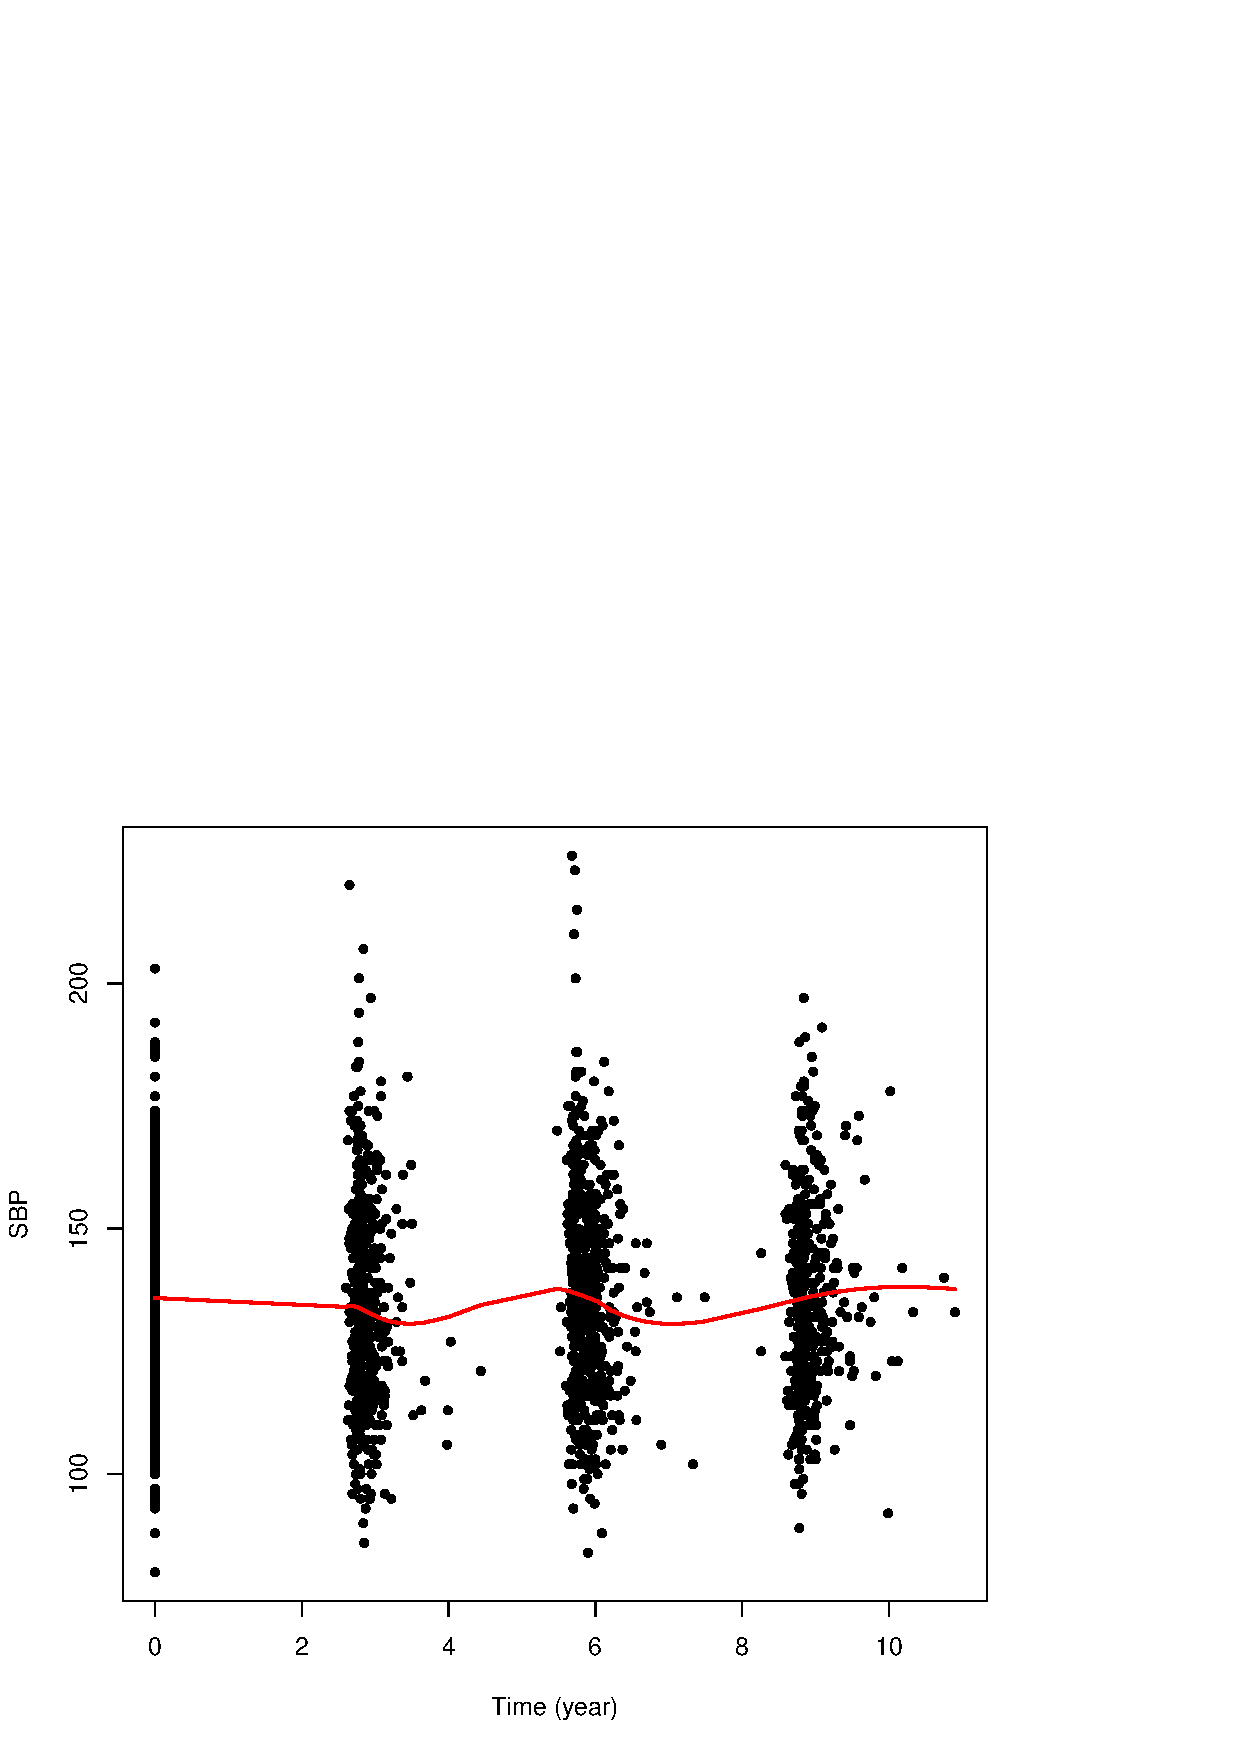
\includegraphics[width=\columnwidth]{SBP_loess.pdf}
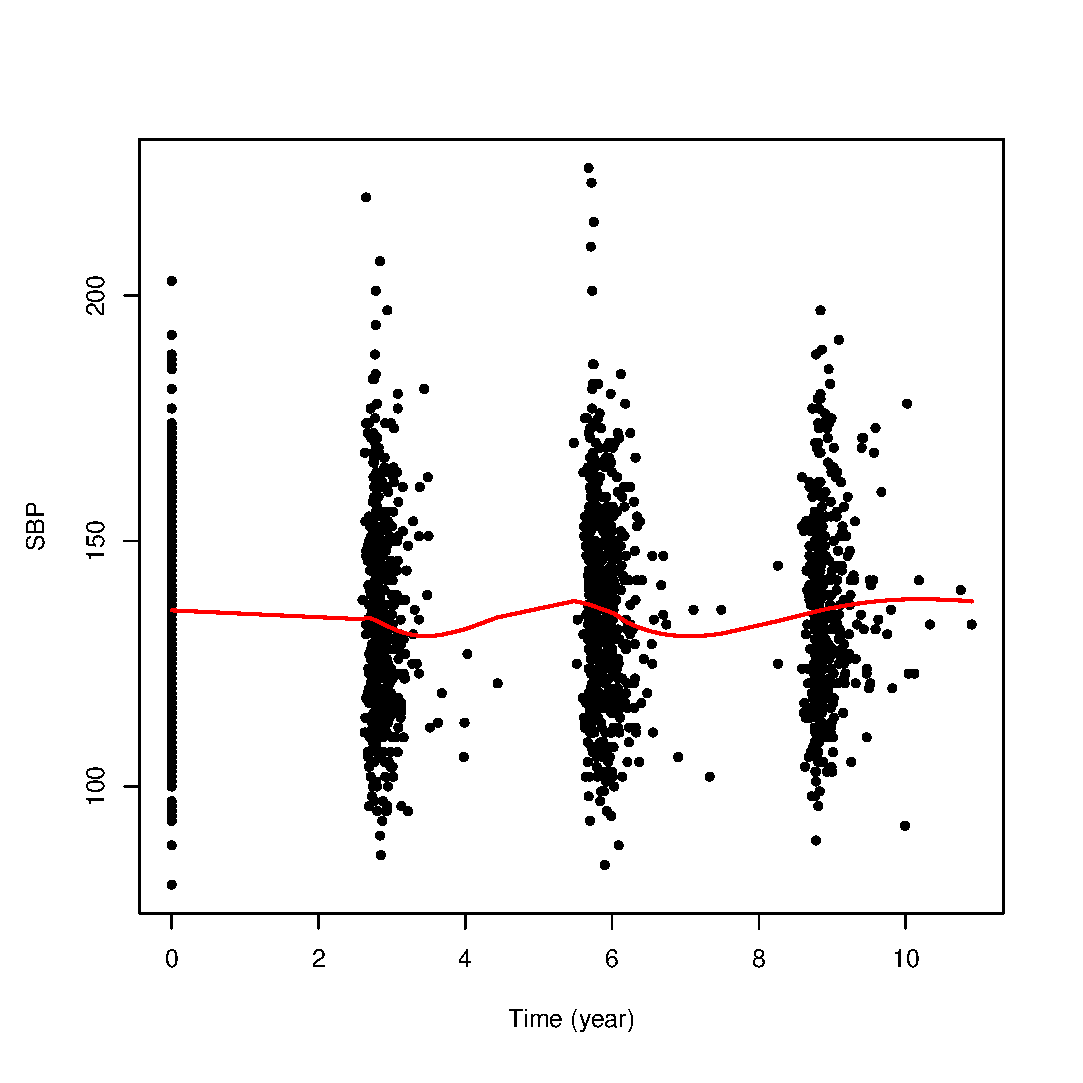
\includegraphics[scale=0.6]{SBP_loess.eps}
\caption{Scatter plot with LOESS curve of longitudinal SBP measures in the study cohort.}
\label{fig:sbp_loess}
\end{figure}

In data analysis, follow-up time is converted from days to years and the first examination date is set to time 0; baseline age is centered by subtracting the overall mean, and total-cholesterol is standardized to have mean 0 and standard deviation 1. We consider the following JM:
\small{
\begin{equation*}\label{eqn:p3data_joint}
\left\{
\begin{array}{l}
sbp_{i}(t) = m_{i}(t) + \varepsilon_{i}(t) = \beta_0 + \beta_1 age_{0i} + \beta_2 chol_i + \beta_3 I_{hyper-med_i}+ \beta_4 t + {u}_{i1} + u_{i2} t + \varepsilon_{i}(t)\\
r_i(t|\mathcal{M}_{i}(t);  \boldsymbol{\gamma}, \alpha) = r_{0}(t)v_i\exp(\gamma_1 I_{male_i} + \gamma_3 I_{smoke_i} + \gamma_4I_{diabetes_i} + \alpha m_i(t))
\end{array}
\right.
\end{equation*}
}
where we assume  $\varepsilon_{i}(t)\sim ALD(0, \sigma, \tau)$. $age_0$ is the baseline age at the first examination, $chol$ stands for the total-cholesterol level (mg/dL), $I_{hyper-med}$ is the variable indicating whether an individual had taken hypertension lowering medication, $t$ is the follow-up time, and $u_{i1}$ and $u_{i2}$ are subject-specific random intercept and slope to account for the within subject correlation and between subject variation. In the recurrent events submodel, we specify a piecewise constant baseline intensity function with three time intervals, where $\lambda_k$ is the hazard rate for time interval $[t_{k-1}, t_{k})$, that is $I_k(t)=1$ if $t\in[t_{k-1}, t_{k})$ and 0 otherwise. Knots $t_1$ and $t_2$, used to define piecewise constant time intervals, are selected as the 33.3\% and 66.7\% percentiles of the ordered follow-up time; while $t_0$ = 0 and $t_3$ is the maximum of follow-up time. We also include a frailty term $v_i$ in the recurrent events model that introduces correlation of multiple CHD events within the same individual. Other model covariates include indicator variables for male ($I_{male}$), ever smoke ($I_{smoke}$), and diabetes mellitus ($I_{diabetes}$). In above QRJM, the true underlying longitudinal measure of SBP is treated as a time dependent covariate in the recurrent event process and $\alpha$ is the association parameter governing the dependence between these two processes. Two chains with diverse initial values are initiated in the Bayesian inference algorithm and the chains are considered to converge if the potential scale reduction factors (PSRF) for all parameters are below 1.1.

We select 80\% of the study cohort (i.e. 526 subjects) to draw parameter inference, based on which we then make predictions of CHD event probability for the rest 131 individuals. Inference results and interpretation can be found in Appendices Table~\ref{p3realdata_inference} and will not be discussed further here. In stead, we focus on presenting the predictions result in the following subsection.


\subsubsection{Dynamic Predictions of Recurrent CHD Event Risk}\label{sec:p3data_results}
To demonstrate how the model works in making subject-specific dynamic predictions of recurrent CHD event risk (in terms of event-free probability), we select three subjects (4, 55, and 65) with distinct data features as the representatives. Figure~\ref{plot:p3realdata_pred_surv_qt50} has three panels with increasing follow-up time in years. For each follow-up time $t$, we make predictions of CHD event-free probability for 1, 2, and 3 years in the future. There are some interesting findings that we would like to highlight: (i) patients who had more CHD events are predicted to have higher risk of CHD recurrence in the future. For example, subject 55 had three CHD events (the most among the three subjects) before year 9 and his/her predicted event-free probability is the lowest (or the highest risk) among the three, followed by subject 65, who had only one event. And subject 4, who didn't have any event occur at year 9, is predicted to only have small probabilities of CHD event in the near future. (ii) With longer follow-up time but no additional event, the predicted event-free probability improves. For example, in subject 55, there is no additional event occurs from $t=12$ to $t=14$ and the predicted event-free probabilities based on $t=14$ are higher than those from $t=12$ for the same $t+\Delta t$ values. (iii) Wider credible interval for larger prediction time window. This makes sense as the prediction uncertainty is higher for further time in the future.

Furthermore, we make the predictions for the whole testing data with three conditional quantiles (0.25, 0.50, and 0.75) of SBP. We summarize the predictive accuracy and present it in Table~\ref{tab:p3data_auc} using AUC, AARD and MRD. First, for the same follow-up time $t$, predictive accuracy is best with smallest $\Delta t$ and decreases when $\Delta t$ increases. This is probably because in this data set majority of the patients didn't have any event observed during the study follow-up and the predicted event-free probability didn't decrease significantly with larger $\Delta t$, thus it is more difficult for the model to differentiate those who will versus who will not have CHD event in the longer future since the predictions are close to each other. Second, with longer follow-up time, the predictive accuracy improves accordingly. This finding is consistent with what we observed in the simulation study and it probably dues to the effect of additional longitudinal and recurrent events information used in making predictions. In additional, we also calculate the AUC for the predictions made from the traditional LMJM model. Compared with LMJM, QRJM has better predictive accuracy at some quantiles, but not all. This is because some conditional quantiles of the SBP can be more informative in predicting future recurrent events than the conditional mean while some are not.


\begin{figure}[H]
\captionsetup[subfloat]{farskip=-5pt,captionskip=-1pt}
\centering
\subfloat[Predictions based on follow-up time $t = $ 9]{
    \includegraphics[width=\columnwidth]{qt50_80pct_t9_dt123456.pdf}\label{plot:p3realdata_pred_surv_t9}
}

\centering
\subfloat[Predictions based on follow-up time $t=$ 12]{
    \includegraphics[width=\columnwidth]{qt50_80pct_t12_dt123456.pdf}\label{plot:p3realdata_pred_surv_t16}
}

\centering
\subfloat[Predictions based on follow-up time $t=$ 14]{
    \includegraphics[width=\columnwidth]{qt50_80pct_t14_dt123456.pdf}\label{plot:p3realdata_pred_surv_t18}
}
  \caption{ARIC data analysis: Dynamic predictions of CHD event-free probability, based on various follow-up time and prediction time window, with 95\% credible interval from QRJM at $\tau=0.5$ for selected subjects ($*$ indicates CHD event).}
  \label{plot:p3realdata_pred_surv_qt50}
\end{figure}





\begin{table}[H]
\centering
\caption{ARIC data analysis: AUC, AARD and MRD of the predictions of CHD event-free probability from QRJM and AUC from LMJM.}
\label{tab:p3data_auc}
\adjustbox{max width=\textwidth}{
\begin{tabular}{rrrrrrrrrrrrrrc}
\hline
$t$ & $\Delta t$ & \multicolumn{3}{c}{AUC ($\tau$)} & & \multicolumn{3}{c}{AARD ($\tau$)} & & \multicolumn{3}{c}{MRD ($\tau$)} & & \multirow{2}{*}{AUC (LMJM)}\\
\cline{3-5}  \cline{7-9} \cline{11-13}
\multicolumn{2}{c}{(year)}  & 0.25 & 0.50 & 0.75 & & 0.25 & 0.50 & 0.75 & & 0.25 & 0.50 & 0.75 & & \\
\hline
\multirow{3}{*}{$9$}  & 1 & 0.726 & 0.713 & 0.712 && 0.357 & 0.327 & 0.327 &&  0.035 & 0.032 & 0.034 & &0.717\\
            & 2 &  0.685 & 0.671 & 0.670 &&  0.286 & 0.255 & 0.255 && 0.028 & 0.024 & 0.025 && 0.676\\
            & 3 &  0.669 & 0.654 & 0.654 &&  0.257 & 0.227 & 0.228 && 0.027 & 0.022 & 0.023  & &0.659\\[0.5em]
\multirow{3}{*}{$12$}  & 1 & 0.770 & 0.756 & 0.754  && 0.434 & 0.402 & 0.400 &&  0.056 & 0.053 & 0.053 & &0.761\\
            & 2 &  0.721 & 0.703 & 0.703 && 0.345 & 0.303 & 0.304 && 0.044 & 0.039 & 0.039 & &0.710\\
            & 3 & 0.699 & 0.680 & 0.680 &&  0.307 & 0.266 & 0.267 && 0.042 & 0.035 & 0.035 & &0.687\\[0.5em]
\multirow{3}{*}{$14$}  & 1 &  0.797 & 0.784 & 0.784 &&  0.487 & 0.463 & 0.464 && 0.071 & 0.068 & 0.069 & &0.789\\
            & 2 & 0.748 & 0.731 & 0.732  && 0.394 & 0.355 & 0.357  &&  0.059 & 0.054 & 0.054 & &0.738\\
            & 3 &  0.714 & 0.695 & 0.697 && 0.331 & 0.288 & 0.293  && 0.059 & 0.049 & 0.050 & &0.704\\
\hline
\end{tabular}
}
\end{table}










% \end{document}

% \documentclass{article}
% \usepackage[utf8]{inputenc}
% \usepackage{fullpage}
% \usepackage {setspace}
% \usepackage[hang,flushmargin]{footmisc} %control footnote indent
% \usepackage{url} % for website links
% \usepackage{amssymb,amsmath}%for matrix
% \usepackage{graphicx}%for figure
% \usepackage{appendix}%for appendix
% \usepackage{float}
% \usepackage{multirow}
% \usepackage{longtable}
% \usepackage{morefloats}%in case there are too many float tables and figures
% \usepackage{caption}
% \usepackage{subcaption}
% \usepackage{listings}
% \captionsetup[subtable]{font=normal}
% \usepackage{color}
% \usepackage{hyperref}
% \usepackage[round]{natbib}
% \usepackage{appendix}
% \usepackage{listings}
% \usepackage{courier}
% \usepackage{color}


% \lstset{style=mystyle}


% \setlength{\parindent}{0em}
% \setlength{\parskip}{0.5em}


% \graphicspath{{0.plots/}}



% \begin{document}



\subsection{Discussion}\label{sec:p3discussion}
In this work, we develop a Bayesian algorithm to make subject-specific dynamic predictions of recurrent event probability based on a new version of JM that uses LQMM for the longitudinal outcome , i.e. QRJM. Derivation of the Bayesian algorithm is based on the location-scale representation of the ALD for the longitudinal quantile regression. The Bayesian algorithm, which is straightforwardly implemented in \textsf{JAGS} software, uses a piecewise constant baseline hazard function in the recurrent events submodel. However, other functional forms can also be considered and the integration of the hazard function can be approximated using numerical integration such as Simpson's rule. Moreover, our predictions of recurrent event probability are based on the entire longitudinal trajectory as well as the recurrent events history of a subject and can be dynamically updated when new data from either (or both) outcome is available. In the real data application, we illustrate the flexibility of the QRJM and its advantages over the LMJM by jointly modeling the risk of CHD recurrences and longitudinal SBP measurements. QRJM is able to provide more insight into the disease progression and the association between the two disease processes in terms of various quantile-based estimations and dynamic predictions.

The significance of current work can be interpreted from two perspectives. First of all, the idea of personalized dynamic predictions of recurrent event probability finds its practical importance in disease control and prevention. Event prediction using commonly collected biomarkers can provide clinicians with continuously updated ``disease progression'' information potentially allowing them to make appropriately timed intervention decisions for individual subjects. Utilizing the dynamic predictions based on the proposed QRJM framework, we obtain subject-specific predictions of event risk that would actually allow physicians to target or tailor medical treatment based on a specific patient profile. In addition, our novel extension of traditional JM with LQMM adds more flexibility to the modeling framework and allows us to investigate specific subgroup of patients of interest. One one hand, patients with extremer biomarker measurements are usually at higher risk of disease thus deserve additional attention in health care. On the other hand, if treatment effect on tails of the outcome is significantly different from the average effect, treatment strategy should also be adjust accordingly to achieve better clinical outcome.

In summary, the QRJM proposed in this paper is a good alternative to the LMJM when either the normality assumption of the errors term is concerned or the conditional quantiles are more relevant to research question. And the dynamic predictions algorithm can be a highly potent tool in personalized disease control and prevention. The current version of QRJM uses LQMM and Cox PHM for the longitudinal and recurrent event processes respectively. However, other functional forms for both outcomes can also be considered to extend the proposed method. For example, in the longitudinal process, nonlinear QR \citep{koenker1996interior} or even nonparametric QR \citep{le2005nonparametric} models can be used to free the assumption of linearity. In the recurrent events submodel, accelerated failure time model can be considered when the proportionality assumption is violated and counting process approach is another nonparametric option.

% In summary, the QRJM is a good alternative to the LMJM when either the normality assumption of the errors term is concerned or the conditional quantiles are more relevant to research question. When the interest lies in the prediction of future recurrent event probability, the ``best'' quantile may be chosen based on the predictive accuracy criteria. Other model selection methods or methods, e.g., Bayesian model averaging, to incorporate multiple regression results from different quantiles into a single prediction solution can be a potential direction for future work. However, in our opinion, the choice of specific quantile(s) should be more clinically oriented rather than be a statistical task.

% A question arises naturally from using quantile regression is which quantile should we choose? The answer is not unique and should depend on the specific research aim.

%All is done in \LaTeX \cite{knuth1986texbook}.
%
%
% \bibliographystyle{plainnat}%%%%%%%%%%%%%%%%%%%%
% \addcontentsline{toc}{section}{References}
% \bibliography{QRJM}


% \end{document}

\newpage
% \documentclass[12pt]{article}
% \usepackage[text={7.1 in, 8 in}, top=1.75in, left=0.69in]{geometry}
% \usepackage[round]{natbib}
% \usepackage[utf8]{inputenc}
% \usepackage{fullpage}
% \usepackage {setspace}
% \usepackage[hang,flushmargin]{footmisc} %control footnote indent
% \usepackage{url} % for website links
% \usepackage{amssymb,amsmath}%for matrix
% \usepackage{graphicx}%for figure
% \usepackage{appendix}%for appendix
% \usepackage{float}
% \floatstyle{plaintop}
% \restylefloat{table}
% \usepackage{multirow}
% \usepackage{longtable}
% \usepackage{morefloats}%in case there are too many float tables and figures
% \usepackage{caption}
% % \usepackage{subcaption}
% \usepackage{subfig}
% \captionsetup[subtable]{font=normal}
% \usepackage{hyperref}
% \usepackage{courier}
% \usepackage{color}
% \usepackage{setspace}
% \usepackage{rotating} % rotate table by some degree
% \usepackage{rotfloat}
% \usepackage{mwe}
% \usepackage{listings}
% \usepackage{titling}
% \usepackage{lipsum}
% \usepackage[export]{adjustbox}




% \graphicspath{{figures/}}

% \begin{document}
% \author{\small{\bf Ming Yang, Sheng Luo,
% and Stacia M. DeSantis}\\
% \small{Department of Biostatistics, The University of Texas Health Science Center at Houston}}
% \date{}
% \title{\large{\bf Web-based Supplementary Material for ``Model Estimation and Dynamic Prediction in Joint Modeling Using Longitudinal Quantile Regression''}}
% \maketitle{}

% \thispagestyle{lscape}
% \begin{landscape}

\subsection*{Appendices}
\addcontentsline{toc}{subsection}{Appendices}
\renewcommand{\thesubsubsection}{\Alph{subsubsection}}
\setcounter{subsubsection}{0}
\subsubsection{Additional Simulation Results}\label{apped:p3_sim}
\doublespacing
% \begin{sidewaystable}[H]
\begin{table}[H]
\centering
\caption{Simulation study: Inference results for data generated from various error distributions\textsuperscript{*}.}
\label{tab:p3sim_inference}
\resizebox{\linewidth}{!}{
\begin{tabular}{lccccccccccccccccccc}
\hline
& \multicolumn{4}{c}{$ALD$(0, 1, 0.25)} & & \multicolumn{4}{c}{$ALD$(0, 1, 0.50)} & & \multicolumn{4}{c}{$ALD$(0, 1, 0.75)}& & \multicolumn{4}{c}{$\mathcal{N}$(0, 1)}\\
\hline
& Bias & SE & MSE & CP & & Bias & SE &  MSE & CP & & Bias & SE & MSE & CP & & Bias & SE & MSE & CP\\
&  \multicolumn{12}{l}{Coefficients for longitudinal process}\\
$\beta_1$ & $-$0.001 & 0.064 & 0.004 & 0.920 & & $-$0.001 & 0.061 & 0.004 & 0.920 & & $-$0.005 & 0.064 & 0.005 & 0.940 & & 0.000 & 0.054 & 0.003 & 0.930 \\
$\beta_2$ & $-$0.003 & 0.116 & 0.011 & 0.970 & & $-$0.002 & 0.113 & 0.011 & 0.965 & & $-$0.001 & 0.116 & 0.015 & 0.920 & & 0.006 & 0.106 & 0.012 & 0.940 \\
$\beta_3$ & 0.020 & 0.048 & 0.003 & 0.950 & & 0.015 & 0.044 & 0.002 & 0.950 & & 0.027 & 0.048 & 0.003 & 0.900 & & 0.009 & & 0.009 & 0.027 & 0.001 & 0.920\\
$\sigma$ & 0.001 & 0.022 & 0.001 & 0.970 & & 0.002 & 0.022 & 0.001 & 0.940 & & 0.003 & 0.022 & 0.001 & 0.940 & & $-$ & $-$ & $-$ & $-$ \\
&  \multicolumn{12}{l}{Coefficients for recurrent event process}\\
$\gamma$ & 0.007 & 0.052 & 0.004 & 0.920 & & 0.008 & 0.050 & 0.003 & 0.915 & & 0.005 & 0.052 & 0.002 & 0.955 & & $-$0.007 & 0.037 & 0.002 & 0.930 \\
$r_0$ & $-$0.017 & 0.093 & 0.008 & 0.940 & & $-$0.016 & 0.087 & 0.008 & 0.940 & & $-$0.003 & 0.096 & 0.010 & 0.935 & & 0.022 & 0.063 & 0.006 & 0.900 \\
$\alpha$ & 0.003 & 0.051& 0.003 & 0.950  & & 0.003 & 0.047 & 0.003 & 0.940 & & 0.001 & 0.051 & 0.003 & 0.940 & & $-$0.014 & 0.033 & 0.002 & 0.850 \\
\hline
\multicolumn{16}{l}{\textsuperscript{*}\footnotesize{data are fitted with true model for ALD distributed error and with ALD(0, 1, 0.50) for standard normal error.}}\\
\end{tabular}

}
\end{table}
% \end{sidewaystable}
% \end{landscape}
% \restoregeometry
% \pagestyle{plain}


% \thispagestyle{lscape}
% \begin{landscape}
\renewcommand{\thesubsubsection}{\Alph{subsubsection}}
\doublespacing

\setcounter{subsubsection}{1}
\subsubsection{Study Cohort Characteristics}
\begin{table}[H]
\centering
\caption{Baseline characteristics of study cohort with stratification by SBP level}
\label{tab:p3cht_baseline}
\resizebox{\linewidth}{!}{
\begin{tabular}{llcccc}
\hline
& & \multicolumn{3}{c}{SBP groups (mm Hg)} \\
\cline{3-5}
 Characteristics\textsuperscript{$\dagger$} & Total ($n=$ 657) & $<$ 120 ($n=$ 133, 20.2\%)  & [120, 140) ($n=$ 217, 33.0\%)& $\ge$ 140 ($n=$ 307, 46.7\%) & $p$-value\textsuperscript{*}\\
 \hline
 Age & 56.4 (5.8) & 55.0 (5.7) & 55.7 (6.0) & 57.4 (5.4) & $<$0.001\\
 SBP & 135.9 (18.5) & 110.5 (6.9) & 129.2 (5.7) & 151.6 (11.2) & $<$0.001\\
 Cholesterol (mg/dL)& 215.9 (41.7) & 215.1 (42.1) & 214.0 (42.0) & 217.6 (41.7) & 0.60 \\
 Gender (male) & 341 (51.9) & 64 (48.1) & 117 (53.9) & 160 (52.1) & 0.57\\
 Ever smoke (yes) & 379 (57.5) & 81 (60.9) & 126 (58.1) & 172 (56.0) & 0.63\\
 Hypertension medication (yes) & 445 (67.7) & 132 (99.2) & 196 (90.3) & 117 (38.1) & $<$0.001\\
 Diabetes (yes) & 90 (13.7) & 15 (11.3) & 27 (12.4) & 48 (15.6) & 0.38\\
   \hline
   \multicolumn{6}{l}{\textsuperscript{$\dagger$}\footnotesize{mean (sd) for continuous variables and frequency (percentage) for categorical variables.}}\\
   \multicolumn{6}{l}{\textsuperscript{*}\footnotesize{Comparing three SBP groups; ANOVA test for continuous variables and $\chi^2$ test for categorical variables.}}\\
\end{tabular}
}
\end{table}

% \end{landscape}
% \restoregeometry
% \pagestyle{plain}
\renewcommand{\thesubsubsection}{\Alph{subsubsection}}

\subsubsection{Inference Results for ARIC Data}\label{sec:p3data_inference}
Inference results for five different quantiles (0.05, 0.25, 0.50, 0.75, and 0.95) are shown in Table~\ref{p3realdata_inference}. In the longitudinal SBP process, older participants generally have higher SBP level and this effect of baseline age is consistently positive across five quantiles of SBP. For example, one year increase in baseline age is associated with 0.036 (95\% CI: (0.026, 0.047)) unit increase in the median (i.e., $\tau=0.50$) of standardized SBP in the study cohort when controlling for other covariates. Total cholesterol level is negatively associated with SBP; however, the effects are not significant for all five quantiles. In general, people who took hypertension medications have significantly lower SBP and the effect of taking hypertension medications increases as the SBP level increases. It is interesting to see that time has a significantly positive effect on higher quantile of SBP (i.e., $\tau=0.75$ and 0.95) while for lower quantiles ($\tau=0.05$, 0.25, and 0.50) the effect is not significant. This can be an important indication that among the hypertension patients who originally have higher SBP deteriorate even faster than those with lower SBP.

In the recurrent CHD event process, we see all positive association between the five conditional quantiles of SBP and the risk of CHD event, which coincide with our expectation as well as previous studies using ARIC data. While the degree of association varies among the conditional quantiles and is strongest on the conditional median of SBP (relative risk:1.25, 95\% CI: (1.02, 1.53)) in our case. For other regression covariates, diabetic patients are at significantly higher risk of having recurrent CHD event compared with non-diabetic. For example, when controlling for other factors, at $\tau=0.5$ the risk of having additional CHD event is 2.6 times higher ($\exp(0.95)$, 95\% CI: (1.57, 4.45)) for people with diabetes than those who are free of the disease. Although, males and ever smokers are also at higher risk of experiencing CHD events, the effects are not statistically significant compared with females and never smokers respectively.

\newpage
% \thispagestyle{lscape}
% \pagestyle{lscape}
% \begin{landscape}
% \doublespacing
% \begin{sidewaystable}[H]
\begin{table}[H]
\centering
\caption{ARIC data analysis: Parameter estimation and 95\% credible interval (in parenthesis) from the QRJM at five quantiles with SBP as the longitudinal biomarker.}
\label{p3realdata_inference}
\resizebox{\linewidth}{!}{
\begin{tabular}{lccccc}
  \hline
  & $\tau=0.05$ & $\tau=0.25$ & $\tau=0.50$ & $\tau=0.75$ & $\tau=0.95$\\
\hline
\multicolumn{6}{l}{{Coefficients for longitudinal SBP process}}  \\
  Intercept & $-$0.374  & $-$0.023  & 0.447  & 0.872  &1.187 \\
  & ($-$0.478, $-$0.274) & ($-$0.118, 0.074) & (0.352, 0.554) & (0.775, 0.978) & (1.079, 1.300)\\
  Age$_0$ & 0.035 & 0.034  & 0.037  & 0.040  & 0.043 \\
  & (0.026, 0.044) & (0.025, 0.044) & (0.028, 0.047) & (0.030, 0.050) & (0.031, 0.052)\\
  Total cholesterol (mg/dL) & $-$0.020  & $-$0.026  & $-$0.022 & $-$0.013 & $-$0.022 \\
  & ($-$0.073, 0.033) & ($-$0.081, 0.032) & ($-$0.078, 0.037) & ($-$0.073, 0.047) & ($-$0.076, 0.032)\\
  Hypertension medicine & $-$0.583  & $-$0.652 & $-$0.725 & $-$0.730 & $-$0.787\\
  &  ($-$0.710, $-$0.467) & ($-$0.773, $-$0.538) &  ($-$0.842, $-$0.609) &  ($-$0.868, $-$0.593) &  ($-$0.924, $-$0.660)\\
  Follow-  up time (yr) & 0.008  & 0.006 & 0.011  & 0.016  & 0.019 \\
  &($-$0.003, 0.018) & ($-$0.006, 0.019) & ($-$0.001, 0.022) & (0.004, 0.029) & (0.005, 0.033)\\\\
  \multicolumn{6}{l}{{Coefficients for recurrent CHD process}}  \\
  Male & 0.191  & 0.185  &  0.160  & 0.132  & 0.110 \\
  & ($-$0.152, 0.548) & ($-$0.170, 0.528) &  ($-$0.187, 0.507) & ($-$0.205, 0.477) & ($-$0.234, 0.458)\\
  Ever smoke & 0.291 & 0.271 & 0.216 & 0.165 & 0.163\\
  & ($-$0.044, 0.641) & ($-$0.070, 0.613) &  ($-$0.121, 0.552) & ($-$0.177, 0.493) &  ($-$0.184, 0.485)\\
  Diabetes & 0.918 & 0.895 & 0.850 & 0.811 & 0.818\\
  & (0.424, 1.399) & (0.409, 1.376) & (0.381, 1.349) & (0.352, 1.318) & (0.333, 1.301)\\
  Association & 0.163 & 0.207  & 0.226  &  0.205  &0.162 \\
  &  ($-$0.003, 0.332) &  (0.011, 0.405) &  (0.019, 0.428) &   (0.034, 0.374) & (0.028, 0.288)\\
   \hline
\end{tabular}
}
\end{table}
% \end{sidewaystable}
% \end{landscape}
% \restoregeometry
% \pagestyle{plain}



\subsubsection{\textsf{JAGS} Model File for Bayesian Inference}
\textsf{JAGS} model file to fit QRJM of longitudinal and recurrent event data.
{\scriptsize
\begin{verbatim}
model{
      k1 <- (1-2*qt)/(qt*(1-qt))
      k2 <- 2/(qt*(1-qt))

      # prior of random effects
      for (i in 1:I){ # I: unique subject id
        # prior for random effects
          u[i] ~ dnorm(0, tau)
      } # end of loop i

      # longitudinal process, BQR mixed model using ALD representation
      for (j in 1:N_l){ # N_l: number of longitudinal observations
          er[j] ~ dexp(sigma)
          mu[j] <- beta1*X1_l[j] + beta2[X2_l[j]] + beta3*t[j] + u[id_l[j]]
          			+ k1*er[j]
          prec[j] <- sigma/(k2*er[j])
          y[j] ~ dnorm(mu[j], prec[j])
      } #end of j loop

    # recurrent events part, baseline hazard is set to constant c
      for(k in 1:I){
        for (l in (s[k]+1):s[k+1]){
          m1[l] <- beta1*X1[k]+beta2[X2[k]]+beta3*Ri1[l]+u[id_r[l]]
          m2[l] <- beta1*X1[k]+beta2[X2[k]]+beta3*Ri2[l]+u[id_r[l]]
          res[l] <- (exp(gamma*W[k]+alpha*m2[l])
                       -exp(gamma*W[k]+alpha*m1[l]))/(alpha*beta3)
          S[l] <- exp(-c*res[l])
          risk[l] <- c*exp(gamma*W[k] + alpha*m2[l])
          L[l] <- pow(risk[l], event[l])*S[l]/1E+08
          zeros[l] ~ dpois(-log(L[l]))
        } # end of l loop
      }#end of k loop

    # priors for other parameters
      alpha ~ dnorm(0, 0.001)
      beta1 ~ dnorm(0, 0.001)
      beta2[1] <- 0
      beta2[2] ~ dnorm(0, 0.001)
      beta3 ~ dnorm(0, 0.001)
      gamma ~ dnorm(0, 0.001)
      sigma ~ dgamma(0.001, 0.01)
      c ~ dunif(0.01, 10)
      tau <- pow(var, -2)
      var ~ dunif(0, 1000)
  }
\end{verbatim}
}

\addcontentsline{toc}{subsection}{References}
\putbib[paper3]
\end{bibunit}

%%%%%%%%%%%%%%%%%%%% reference %%%%%%%%%%%%%%%%%%%%
\newpage
\bibliographystyle{apa}
\addcontentsline{toc}{section}{References}
\bibliography{Phdthesis_background}

\end{document}